\documentclass[11pt]{book}
%-------------------PAQUETES-------------------------------
\usepackage{graphicx}
\usepackage[spanish]{babel}
\usepackage{verbatim}
\usepackage{listings}
\usepackage{color}
\usepackage[cache=false]{minted}
\usemintedstyle{coloso}
\usepackage{longtable} 
\usepackage[utf8]{inputenc}
\usepackage{array}
\usepackage{hyperref}
%---------------COMANDOS--------------------
\newcommand{\imagen}[3]{
\begin{figure}[h!]
	\centering
	\includegraphics[width=#1\linewidth]{#2}
	\caption{#3}
\end{figure}
}
%-------------------------------------------
\definecolor{miverde}{rgb}{0,0.6,0}
\definecolor{migris}{rgb}{0.5,0.5,0.5}
\definecolor{mimalva}{rgb}{0.58,0,0.82}

\lstset{ %
	backgroundcolor=\color{white},   % Indica el color de fondo; necesita que se añada \usepackage{color} o \usepackage{xcolor}
	basicstyle=\footnotesize,        % Fija el tamaño del tipo de letra utilizado para el código
	breakatwhitespace=false,         % Activarlo para que los saltos automáticos solo se apliquen en los espacios en blanco
	breaklines=true,                 % Activa el salto de línea automático
	captionpos=b,                    % Establece la posición de la leyenda del cuadro de código
	commentstyle=\color{miverde},    % Estilo de los comentarios
	deletekeywords={...},            % Si se quiere eliminar palabras clave del lenguaje
	escapeinside={\%*}{*)},          % Si quieres incorporar LaTeX dentro del propio código
	extendedchars=true,              % Permite utilizar caracteres extendidos no-ASCII; solo funciona para codificaciones de 8-bits; para UTF-8 no funciona. En xelatex necesita estar a true para que funcione.
	frame=single,	                   % Añade un marco al código
	keepspaces=true,                 % Mantiene los espacios en el texto. Es útil para mantener la indentación del código(puede necesitar columns=flexible).
	keywordstyle=\color{blue},       % estilo de las palabras clave
	language=Java,                 % El lenguaje del código
	otherkeywords={*,...},           % Si se quieren añadir otras palabras clave al lenguaje
	numbers=left,                    % Posición de los números de línea (none, left, right).
	numbersep=5pt,                   % Distancia de los números de línea al código
	numberstyle=\small\color{migris}, % Estilo para los números de línea
	rulecolor=\color{black},         % Si no se activa, el color del marco puede cambiar en los saltos de línea entre textos que sea de otro color, por ejemplo, los comentarios, que están en verde en este ejemplo
	showspaces=true,                % Si se activa, muestra los espacios con guiones bajos; sustituye a 'showstringspaces'
	showstringspaces=false,          % subraya solamente los espacios que estén en una cadena de esto
	showtabs=true,                  % muestra las tabulaciones que existan en cadenas de texto con guión bajo
	stepnumber=2,                    % Muestra solamente los números de línea que corresponden a cada salto. En este caso: 1,3,5,...
	stringstyle=\color{mimalva},     % Estilo de las cadenas de texto
	tabsize=2,	                   % Establece el salto de las tabulaciones a 2 espacios
	title=\lstname                   % muestra el nombre de los ficheros incluidos al utilizar \lstinputlisting; también se puede utilizar en el parámetro caption
}
\newmintedfile[CodigoJava]{java}{
	%bgcolor= gray!1!white,
	fontsize=\footnotesize,
	fontfamily=tt,	
	linenos=true,
	numberblanklines=true,
	numbersep=3pt,
	gobble=0,
	%frame=bottomline,
	rulecolor = red!20,
	framerule=0.1pt,
	framesep=0mm,
	funcnamehighlighting=true,
	tabsize=4,
	obeytabs=false,
	mathescape=false
	samepage=false, %with this setting you can force the list to appear on the same page
	showspaces=false,
	showtabs =false,
	texcl=false,
	breaklines=true
}

%----------------------------
\newcommand{\plogo}{\fbox{$\mathcal{PL}$}} % Generic dummy publisher logo

%-------------------MACROS---------------------------------
%-------------------PORTADA--------------------------------
\author{
	Nestor David Bohorquez Galeano \\ 
	20172020083 \\
	Nicolas Herrera Rubiano \\
	20171020118 \\
	Alvaro Andres Niño Rincon \\
	20171020139	
}
\title{Arquitectura Empresarial}

\begin{document}
%\maketitle

\begin{titlepage} % Suppresses headers and footers on the title page
	
	\centering
	\scshape % Use small caps for all text on the title page
	\vspace*{\baselineskip} % White space at the top of the page
	
	\rule{\textwidth}{1.6pt}\vspace*{-\baselineskip}\vspace*{2pt} % Thick horizontal rule
	\rule{\textwidth}{0.4pt} % Thin horizontal rule
	
	\vspace{0.75\baselineskip}
	
	{\LARGE ARQUITECTURA EMPRESARIAL} % Title
	
	\vspace{0.75\baselineskip}
	
	\rule{\textwidth}{0.4pt}\vspace*{-\baselineskip}\vspace{3.2pt} % Thin horizontal rule
	\rule{\textwidth}{1.6pt} % Thick horizontal rule
	
	\vspace{2\baselineskip}
	
	\vspace*{3\baselineskip}
	
	Elaborado Por
	
	\vspace{0.5\baselineskip} 
	
	{\scshape\Large Nestor David Bohorquez Galeano \\ 20172020083 \\ 
	Nicolas Herrera Rubiano \\ 20171020118 \\ 
	Alvaro Andres Niño Rincon \\ 20171020139}
	
	\vspace{0.5\baselineskip} 
	
	\textit{Universidad Distrital Francisco José de Caldas}
	
	\vfill 
	
	\begin{figure}[h!]
		\centering
		\includegraphics[width=0.3\linewidth]{imgs/ud.jpeg}
	\end{figure}
	
	\today
\end{titlepage}

\tableofcontents
\listoffigures

\part{PROYECTO}
\section{Punto de Vista de Organización}

El punto de vista de la organización se centra en la organización (interna) de una empresa, un departamento, una red de empresas o de otra entidad organizativa. Es posible presentar modelos en este punto de vista como diagramas de bloques anidados, pero también de una manera más tradicional, como los organigramas. El punto de vista de la organización es muy útil para identificar las competencias, la autoridad y las responsabilidades de una organización.

\subsection{Modelo de Organización}
\begin{figure}[h!]
	\centering
	\includegraphics[width=.6\linewidth]{imgs/modelo/Organizacion}
	\caption{Modelo Organizacion}
\end{figure}

Un actor de negocios es una entidad de negocios que es capaz de realizar un comportamiento. Los actores pueden incluir entidades fuera de la organización real; por ejemplo, clientes y socios. Un actor comercial puede representar a esas entidades comerciales en diferentes niveles de detalle, y puede corresponder tanto a un actor como a una unidad organizativa en el marco del TOGAF. Ejemplos de actores comerciales son los seres humanos, los departamentos y las unidades comerciales. Una colaboración empresarial es un conjunto de dos o más elementos de la estructura activa interna de la empresa que trabajan juntos para llevar a cabo un comportamiento colectivo. Una interfaz de negocios es un punto de acceso en el que se pone a disposición del entorno un servicio comercial. Una interfaz comercial expone la funcionalidad de un servicio comercial a otros roles o actores comerciales. Se suele denominar canal (teléfono, Internet, oficina local, etc.). El mismo servicio comercial puede estar expuesto a través de diferentes interfaces.

\newpage
\subsection{Caso  de Organización}
\begin{figure}[h!]
	\centering
	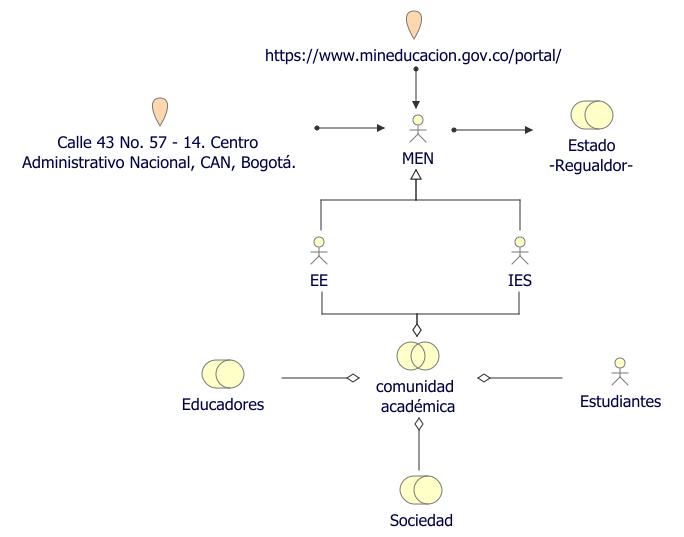
\includegraphics[width=.9\linewidth]{imgs/caso/negocio/organizacion}
	\caption{Caso Organización}
\end{figure}
Un actor de negocios es una entidad de negocios que es capaz de realizar un comportamiento. Los actores pueden incluir entidades fuera de la organización real; por ejemplo, clientes y socios. Un actor comercial puede representar a esas entidades comerciales en diferentes niveles de detalle, y puede corresponder tanto a un actor como a una unidad organizativa en el marco del TOGAF. Ejemplos de actores comerciales son los seres humanos, los departamentos y las unidades comerciales. Una colaboración empresarial es un conjunto de dos o más elementos de la estructura activa interna de la empresa que trabajan juntos para llevar a cabo un comportamiento colectivo. Una interfaz de negocios es un punto de acceso en el que se pone a disposición del entorno un servicio comercial. Una interfaz comercial expone la funcionalidad de un servicio comercial a otros roles o actores comerciales. Se suele denominar canal (teléfono, Internet, oficina local, etc.). El mismo servicio comercial puede estar expuesto a través de diferentes interfaces.

\chapter{Metodología}
\section{Introducción}

El Método de Desarrollo de la Arquitectura de TOGAF (ADM) forma el núcleo del TOGAF.  Es un método fiable y de eficacia probada para desarrollar una arquitectura de TI que satisfaga las necesidades comerciales de una organización, utilizando los demás elementos de TOGAF, y otros activos arquitectónicos disponibles para la organización. \\

El TOGAF consta de dos partes principales:

\begin{itemize}
	\item    El Método de Desarrollo de la Arquitectura de TOGAF (ADM).
	\item La Arquitectura de la Fundación TOGAF, la cual se trata de una arquitectura de servicios y funciones genéricas que proporciona una base firme sobre la que se pueden construir arquitecturas y componentes arquitectónicos más específicos.
\end{itemize}

La ADM de la TOGAF describe el proceso de pasar de la Arquitectura de la Fundación TOGAF a una arquitectura específica de la organización (o conjunto de arquitecturas), aprovechando los elementos de la Arquitectura de la Fundación TOGAF y otros componentes arquitectónicos y bloques de construcción pertinentes a lo largo del camino.\\

La Arquitectura de la Fundación TOGAF no es, por supuesto, el único recurso disponible para el arquitecto en el uso de la ADM. Hay una amplia gama de modelos arquitectónicos, componentes y bloques de construcción relacionados con diferentes aspectos del dominio de la arquitectura. Este contexto mucho más amplio en el que reside la Arquitectura de la Fundación TOGAF se denomina en la TOGAF el Continuo Empresarial.\\

Es importante señalar que, al ejecutar la ADM, el arquitecto no sólo está desarrollando el resultado final de una arquitectura específica de la organización, sino que también está poblando el propio Continuo Empresarial de la organización, con todos los activos arquitectónicos identificados y apalancados a lo largo del camino - incluyendo, pero no limitado a, la arquitectura específica de la organización resultante.\\

Aunque el enfoque principal de la ADM está en el desarrollo de la arquitectura específica de la organización, en este contexto más amplio la ADM también puede verse como el proceso de poblar el Continuo Empresarial de la organización con bloques de construcción reutilizables relevantes.\\

El desarrollo de la arquitectura es un proceso iterativo y continuo, y al ejecutar la ADM repetidamente a lo largo del tiempo, el arquitecto va poblando gradualmente más y más el Continuo Empresarial de la organización.\\

De hecho, la primera ejecución del ADM será a menudo la más difícil, ya que los activos arquitectónicos disponibles para su reutilización serán relativamente pocos. Sin embargo, las ejecuciones posteriores serán más fáciles, ya que cada vez se identifican más activos de arquitectura, que se utilizan para poblar el Enterprise Continuum de la organización y, por lo tanto, están disponibles para su reutilización.

\newpage
\section{ADM}
\begin{figure}[h!]
	\centering
	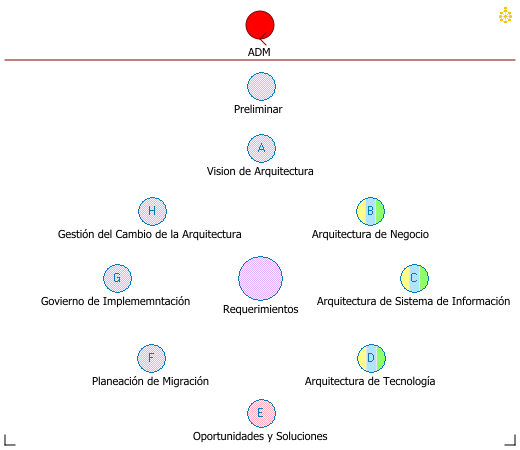
\includegraphics[width=1\linewidth]{imgs/adm.png}
	\caption{ADM \cite{archi3.1,a1,a2,a3,a4}}
\end{figure}

\part{ARQUITECURA}
\chapter{Lenguaje: ArchiMate}
\section{Introducción}
Para el desarrollo de proyectos de ingeniería de software se requiere una serie de componentes, pasos y estructura bien definida que debe seguirse para llevar a buen término la finalización del mismo. Una de estas partes fundamentales en la ingeniería de software es el lenguaje de modelado, el cual es un lenguaje artificial que puede ser utilizado para expresar la información o el conocimiento o sistemas en una estructura que se define por un conjunto coherente de normas. Las reglas se utilizan para interpretar el significado de los componentes de la estructura. Estos lenguajes de modelado pueden ser de dos tipos en específico, el primero es el gráfico, el cual utiliza una técnica de diagrama con símbolos con nombre que representan conceptos y líneas que conectan los símbolos y representan relaciones y varias otras notaciones gráficas para representar restricciones. y el lenguaje textual que puede usar palabras clave estandarizadas acompañadas de parámetros o términos y frases en lenguaje natural para hacer expresiones interpretables por computadora. Entre estos lenguajes de modelado se encuentra uno muy útil el cual es ArchiMate, el cual consiste en un amplio, abierto e independiente lenguaje de modelado con el fin de apoyar la descripción, análisis y visualización de la arquitectura deentro del proyecto de fóma veráz y efectiva. ArchiMate es un estándar técnico de The Open Group y se basa en los conceptos del estándar IEEE 1471 . Cuenta con el respaldo de varios proveedores de herramientas y empresas consultoras. ArchiMate también es una marca registrada de The Open Group. Open Group tiene un programa de certificación para usuarios de ArchiMate, herramientas de software y cursos. ArchiMate se distingue de otros lenguajes como el Lenguaje de modelado unificado (UML) y el Modelado y notación de procesos de negocio (BPMN) por su alcance de modelado empresarial.

\begin{figure}[h!]
	\centering
	\includegraphics[width=0.7\linewidth]{imgs/coreFramwork}
	\caption{Marco completo de ArchiMate}
\end{figure}

\section{Conceptos y su notación}
El lenguaje ArchiMate separa los conceptos del lenguaje (es decir, los constituyentes del metamodelo) de su notación. Diferentes grupos de interesados pueden requerir diferentes notaciones para comprender un modelo o una visión de la arquitectura.  A este respecto, los ArchiMatelanguages de lenguajes como el UML o el BPMN, que sólo tienen una notación normalizada. El mecanismo de punto de vista explicado en el Capítulo 14 proporciona los medios para definir tales visualizaciones orientadas a las partes interesadas. Aunque la notación de los conceptos de ArchiMate puede (y debería) ser específica de las partes interesadas, la norma proporciona una notación gráfica común, que puede ser utilizada por los arquitectos y otros que desarrollan modelos ArchiMate. Esta notación está dirigida a un público acostumbrado a las técnicas de modelización técnica existentes, como ERD, UML o BPMN, y por lo tanto se asemeja a ellas. En el resto de este documento, a menos que se indique lo contrario, los símbolos utilizados para representar los conceptos del lenguaje representan la notación estándar de ArchiMate.  Esta notación estándar para la mayoría de los elementos consiste en un cuadro con un icono en la esquina superior derecha. En varios casos, este icono por sí mismo puede también utilizarse como notación alternativa. Esta iconografía estándar debe preferirse siempre que sea posible para que cualquier persona que conozca el lenguaje ArchiMate pueda leer los diagramas producidos en el lenguaje.

\subsection{Meta}

La principal jerarquía de elementos de comportamiento y estructura del lenguaje ArchiMate se presenta en la tabla 3.1. Define estos elementos de forma genérica e independiente de la capa. Nótese que la mayoría de estos elementos (las cajas blancas) son elementos abstractos del metamodelo; es decir, no están instanciados en los modelos sino que sólo sirven para estructurar el metamodelo.  La notación presentada es, por lo tanto, la forma genérica en que se representan las especializaciones de estos elementos (es decir, los elementos de las diferentes capas de la arquitectura). Además de describir  los elementos concretos (los recuadros grises), que pueden utilizarse para modelar la Arquitectura de la Empresa a nivel estratégico.

\newpage
\subsubsection{Elementos de la Estructura}
	\begin{table}[h!]
	\begin{tabular}{| m{7em} | m{7cm} | m{3cm} |}
		\hline
		Concepto & Descripción & Representación \\
		
		\hline
		Motivación
		& 
		Un elemento de motivación representa el contexto o la motivación detrás de la  arquitectura de la empresa
		& \includegraphics[width=0.8\linewidth, height=0.05\textheight]{imgs/conceptos/meta/Motivacion}
		\\
		
		\hline
		Estructura 
		& 
		Elementos de estructura son equivalentes sinónimos, se subdividen  en estructuras activas ,                              estructuras activas internas,  estructuras activas externas y estructuras pasivas
		& \includegraphics[width=0.8\linewidth, height=0.05\textheight]{imgs/conceptos/meta/Estructura}
		\\
		
		\hline
		Estructura activa  
		& 
		Estructuras que pueden tener un comportamiento
		& \includegraphics[width=0.8\linewidth, height=0.05\textheight]{imgs/conceptos/meta/EstructuraActiva}
		\\  
		
		\hline
		Estructura activa externa  
		& 
		Llamado interfase representa un punto de acceso donde uno o mas servicios son prestados al ambiente  
		&\includegraphics[width=0.8\linewidth, height=0.05\textheight]{imgs/conceptos/meta/EstructuraActivaExterna}
		\\
		
		\hline
		Estructura activa interna
		& 
		Es un elemento que representa una entidad que es capaz de mostrar comportamiento
		& \includegraphics[width=0.8\linewidth, height=0.05\textheight]{imgs/conceptos/meta/EstructuraActivaInterna.PNG}
		\\
		
		\hline
		Estructura pasiva
		& 
		Es un elemento que representa una entidad sobre la cual se realiza un comportamiento
		& \includegraphics[width=0.8\linewidth, height=0.05\textheight]{imgs/conceptos/meta/EstructuraPasiva.PNG}
		\\
		
		\hline
		Interfase
		& 
		Representa un punto de acceso donde uno o mas servicios son puestos en el ambiente.
		& \includegraphics[width=0.8\linewidth, height=0.05\textheight]{imgs/conceptos/meta/Interface.PNG}
		\\
		
		\hline
		
		Comportamiento
		& 
		Es un elemento que equivale a un verbo se  subdivide en evento ,comportamiento interno, proceso , función, interacción, comportamiento externo y servicio.
		& \includegraphics[width=0.8\linewidth, height=0.05\textheight]{imgs/conceptos/meta/Comportamiento.PNG}
		\\
		
		\hline
		Evento
		&
		Representa un cambio de estado 
		& \includegraphics[width=0.8\linewidth, height=0.05\textheight]{imgs/conceptos/meta/Evento.PNG}
		\\
		
		\hline
		Elemento de comportamiento interno 
		& 
		Representa una o mas unidades de actividades que pueden ser realizadas por uno o mas elementos de estructura activa
		& \includegraphics[width=0.8\linewidth, height=0.05\textheight]{imgs/conceptos/meta/ComportamientoInterno.PNG}
		\\	\hline
	\end{tabular}
	%\caption{}
	\label{tab:concepts}
\end{table}

\newpage
\begin{table}[h!]
\begin{center}
	\begin{tabular}{| m{6em} | m{7cm} | m{3cm} |}
		\hline
		Concepto & Descripción & Representación \\ 
		
		\hline
		Servicio
		&
		Un servicio es un comportamiento del sistema proveedor  visible  externamente 
		&
		\includegraphics[width=0.8\linewidth, height=0.05\textheight]{imgs/conceptos/meta/Servicio.PNG}
		\\
		
		\hline
		Función
		& 
		Representa una colección de comportamientos, basado en una colección de criterios específicos, tales como fuente requerida, competencias o localización   
		& \includegraphics[width=0.8\linewidth, height=0.05\textheight]{imgs/conceptos/meta/Funcion.PNG}
		\\
		
		\hline
		Proceso
		& 
		Representa una secuencia de comportamientos que consiguen un resultado especifico
		& \includegraphics[width=0.8\linewidth, height=0.05\textheight]{imgs/conceptos/meta/Proceso.PNG}
		\\
		
		\hline
		Interacción  
		& 
		Representa una unidad de comportamientos que deben ser realizados por dos o mas elementos de estructura activa interna , ya sea a través de una asignación directa o agregados en una colaboración 
		& \includegraphics[width=0.8\linewidth, height=0.05\textheight]{imgs/conceptos/meta/Interaccion.PNG}
		\\
		
		\hline
		Colaboración  
		& 
		Representa un acuerdo entre dos o mas elementos estructuras activas internas, trabajan juntos para realizar algún comportamiento colectivo   
		& \includegraphics[width=0.8\linewidth, height=0.05\textheight]{imgs/conceptos/meta/Colaboracion.PNG}
		\\
		
		\hline
		Elemento de comportamiento externo
		& 
		Representa un comportamiento explicito que es visible en el exterior  
		& \includegraphics[width=0.8\linewidth, height=0.05\textheight]{imgs/conceptos/meta/ComportamientoExterno.PNG}
		\\
		
		\hline
		
		Elementos compuestos 
		&
		Son elementos que se basan en aspectos de otras capas del lenguaje   
		&
		\includegraphics[width=0.8\linewidth, height=0.05\textheight]{imgs/conceptos/meta/Compuesto.PNG}
		\\
		
		\hline
	\end{tabular}
	\caption{Conceptos capa meta}
	\label{tab:concepts}
\end{center}
\end{table}

\chapter{Motivacional}
\label{chap:Motivacional}
\section{Introducción}
Se han definido una serie de puntos de vista estándar para modelar los aspectos motivadores. Cada uno de estos puntos de vista presenta una perspectiva diferente para modelar la motivación que subyace en algunas arquitecturas empresariales y permite al modelador centrarse en ciertos aspectos. Por lo tanto, cada punto de vista considera sólo una selección de los elementos y relaciones que se han descrito en el capítulo 3.

Se distinguen los siguientes puntos de vista:

\begin{itemize}
	\item El punto de vista de los interesados se centra en la elaboración de modelos de los interesados, los factores determinantes, las evaluaciones de esos factores y los objetivos iniciales para abordar esos factores y evaluaciones.
	\item El punto de vista de la realización de los objetivos se centra en el perfeccionamiento de los objetivos iniciales de alto nivel para convertirlos en (sub)objetivos más concretos mediante la relación de agregación y, por último, en requisitos y limitaciones mediante la relación de realización.
	\item El punto de vista de la contribución al logro de objetivos se centra en la modelización y el análisis de las relaciones de influencia entre los objetivos (y los requisitos).
	\item El punto de vista de los principios se centra en la modelización de los principios pertinentes y las metas que motivan esos principios.
	\item El punto de vista de la realización de los requisitos se centra en la modelización de la realización de los requisitos y las limitaciones por medio de elementos básicos, como los agentes, los servicios, los procesos, los componentes de la aplicación, etc.
	\item El punto de vista de la motivación abarca todo el aspecto de la motivación y permite utilizar todos los elementos de motivación.
\end{itemize}

A continuación se describen por separado todos los puntos de vista. Para cada punto de vista, se indican sus elementos y relaciones, las directrices para su utilización, su objetivo y grupo destinatario. Además, la descripción de cada punto de vista contiene modelos de casos.
\newpage

\section{Metamodelo}
\begin{figure}[h!]
	\centering
	\includegraphics[width=1.0\linewidth]{imgs/meta/Motivacion}
	\caption{Metamodelo Motivacional}
\end{figure}

La principal jerarquía de los elementos de comportamiento y estructura del lenguaje ArchiMate se presenta en el metamodelo de la Figura 4.1. Define estos elementos de manera genérica e independiente de la capa. Observe que la mayoría de estos elementos (las cajas blancas) son elementos abstractos del meta modelo; es decir, no están instanciados en los modelos sino que sólo sirven para estructurar el meta modelo.  La notación presentada en este capítulo es, por lo tanto, la forma genérica en que se representan las especializaciones de estos elementos (es decir, los elementos de las diferentes capas de la arquitectura).  Los elementos concretos (las cajas grises), que pueden ser utilizados para modelar la Arquitectura de la Empresa a un nivel estratégico.\\ \\

Este fragmento genérico de metamodelo consiste en dos tipos principales de elementos: elementos de estructura ('sustantivos') y elementos de comportamiento ('verbos').

\newpage
\section{Punto de Vista de Implicados}
El punto de vista de las partes interesadas permite al analista modelar las partes interesadas, los impulsores internos y externos del cambio y las evaluaciones (en términos de fortalezas, debilidades, oportunidades y amenazas) de estos impulsores. También se pueden describir los vínculos con los objetivos iniciales (de alto nivel) que abordan estas preocupaciones y evaluaciones. Estas metas forman la base del proceso de ingeniería de requisitos, incluyendo el refinamiento de las metas, el análisis de la contribución y el conflicto, y la derivación de los requisitos que realizan las metas.

\subsection{Modelo de Implicados}
\begin{figure}[h!]
	\centering
	\includegraphics[width=1.0\linewidth]{imgs/modelo/Interesado}
	\caption{Modelo Implicados}
\end{figure}

Los elementos de motivación se utilizan para modelar las motivaciones, o razones, que guían el diseño o el cambio de una arquitectura empresarial, y es esencial comprender los factores, a menudo denominados impulsores, que influyen en otros elementos de motivación.  Pueden originarse tanto dentro como fuera de la empresa.  Los impulsores internos, también llamados preocupaciones, están asociados con las partes interesadas, que pueden ser algún ser humano individual o algún grupo de seres humanos, como un equipo de proyecto, una empresa o la sociedad. Ejemplos de esos impulsores internos son la satisfacción del cliente, el cumplimiento de la legislación o la rentabilidad. Es común que las empresas realicen una evaluación de esos factores impulsores; por ejemplo, utilizando un análisis FODA, a fin de responder de la mejor manera posible.

%\newpage

\subsection{Caso  de Implicados}
\begin{figure}[h!]
	\centering
	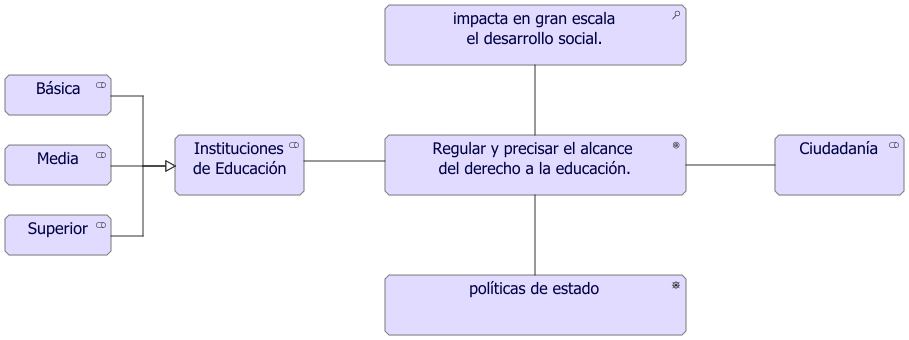
\includegraphics[width=1.0\linewidth]{imgs/motivacion/implicados/imp1.pdf}
	\caption{Caso Implicados}
\end{figure}

Los elementos, principalmente externos que se encuentran fuertemente ligados para regular y precisar el alcance del derecho a la educación, son las políticas de Estado vigentes y en desarrollo dispuestas por la administración a cargo. Por otra parte, la valoración comprendida en este objetivo, impacta en gran medida el desarrollo social del país, debido a que son ellos, la comunidad quienes dispondrán de la oportunidad educarse para forjar un mejor futuro tanto para sus familias como para la comunidad en general. Así mismo, las instituciones de educación básica, media y superior, quienes permiten y promueven la adquisición de habilidades, conocimientos y la ampliación de horizontes personales, a través de los lineamientos dispuestos por el MEN, son otro de los interesados alrededor de este objetivo.
\section{Punto de Vista de la Realización de Objetivos}

El punto de vista de la realización de objetivos permite a un diseñador modelar el refinamiento de los objetivos (de alto nivel) en objetivos más tangibles, y el refinamiento de los objetivos tangibles en requisitos o restricciones que describen las propiedades que se necesitan para realizar los objetivos. El refinamiento de los objetivos en subobjetivos se modela utilizando la relación de agregación. El refinamiento de los objetivos en requisitos se modela utilizando la relación de realización.
Además, se pueden modelar los principios que guían el refinamiento de las metas en requisitos.

\subsection{Modelo de la Realización de Objetivos}
\begin{figure}[h!]
	\centering
	\includegraphics[width=1.0\linewidth]{imgs/modelo/RealObjetivos.pdf}
	\caption{Modelo Realización de Objetivos}
\end{figure}

La motivación de una organización o persona para lograr ciertos resultados está representada por las metas, los principios, los requisitos y las limitaciones. Las metas representan que un interesado quiere lograr un determinado resultado; por ejemplo, "Aumentar la satisfacción del cliente en un 10\%". Los resultados finales obtenidos por las capacidades que realizan estas metas son los resultados.

Un objetivo representa una declaración de intenciones de alto nivel, una dirección o un estado final deseado para una organización y sus partes interesadas.

\newpage

\subsection{Caso de la Realización de Objetivos}
\begin{figure}[h!]
	\centering
	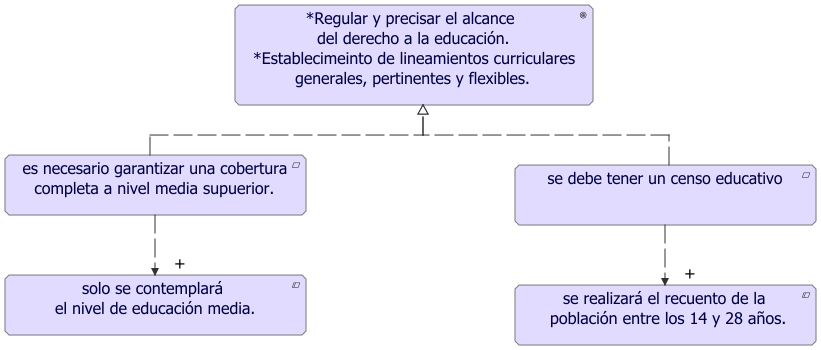
\includegraphics[width=1.0\linewidth]{imgs/motivacion/realizacionObj/realizacion.pdf}
	\caption{Caso Realización de Objetivos}
\end{figure}

Los requerimientos necesarios para regular y precisar el alcance del derecho a la educación, así como para dar alcance al objetivo de establecer los lineamientos curriculares, generales, pertinentes y flexibles radican en garantizar una cobertura completa en la educación media superior del país, que permita abrir una brecha para la implantación de esta ofertas educativas con aras de que logren mantenerse y adquirir una mayor demanda a través de las regulaciones del MEN para dar alcance al derecho de la educación a toda la comunidad. Igualmente, otro requerimiento indispensable para la consecución de estos objetivos planteados, es la realización de un censo educativo que proporcione un conocimiento certero sobre las características de la población a la cual está dirigida esta política inclusiva de educación y que además, provea de información vitalicia para la construcción y/o adecuación de las ofertas educativas de lineamientos curriculares generales, flexibles, pertinentes y flexibles. \\ \\
No obstante, una limitación en el requerimiento dispuesto para la garantía de una cobertura completa a nivel media superior es que, solo se contemplará la identificación vocacional en la transición de un nivel de educación media a superior, postergando la identificación vocacional a través de la gamificación en la transición de educación básica a educación media. A causa de este limitante, el censo educativo, aunque se realizará de forma general, en su etapa posterior del proceso, solo se hará énfasis en el recuento de la población entre los 14 y 28 años.
\section{Punto de Vista de Contribución de Objetivos}
Contribución de objetivos es uno de los puntos de vista de la parte motivacional, este punto de vista permite profundizar y ahondar en los objetivos planteados en el proyecto, con el fin de precisar y aclarar las metas propuestas por medio de una especie de desglose de información. Esta contribución de objetivos como su nombre lo indica, no es única y exclusivamente de un solo objetivo, sino que por el contrario, dependiendo del caso y si hay objetivos relacionados entre si, se pueden agrupar en un solo paquete de objetivo para realizar esta contribución de una manera más personalizada y completa, procurando en todo momento la optimización de todos los recursos.

\subsection{Modelo de Contribución de Objetivos}
\begin{figure}[h!]
	\centering
	\includegraphics[width=1.0\linewidth]{imgs/modelo/ContObjetivos}
	\caption{Modelo Contribución de objetivos}
\end{figure}

El punto de vista de contribución de objetivos, presenta un modelo el cual como su nombre lo indica, se centra en un objetivo del proyecto planteado, del cual se desglosan ciertos requerimientos para este objetivo según sea el caso, sin dejar de mencionar que estos requerimientos pueden presentar en alguna ocasiones ciertas restricciones que son de vital importancia aclarar y mencionar para tener en cuenta en la estructuración del proyecto. Además de esto, siempre en cada modelo se busca un resultado o un fin específico, con este terminaría el punto de vista de contribución de objetivos.

%\newpage

\subsection{Caso  de Contribución de Objetivos}
\begin{figure}[h!]
	\centering
	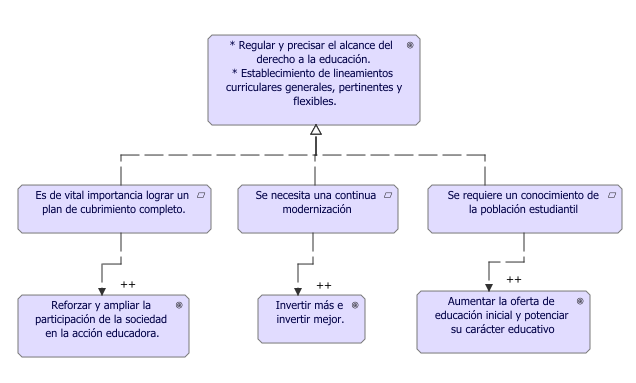
\includegraphics[width=1.0\linewidth]{imgs/motivacion/ContriObjetivos/contriObjetivos.pdf}
	\caption{Caso Contribución de Objetivos}
\end{figure}

En el caso del proyecto planteado, en la sección de objetivos se postularon dos de estos, los cuales son transversales y están estrechamente relacionados, lo cual permite que se puedan trabajar al unisono, estos objetivos son: regular y precisar el alcance del derecho a la educación y establecimiento de lineamientos curriculares generales, pertinentes y flexibles. Ademas de esto, se plantearon tres requerimientos para estos objetivos, el primero de estos requerimientos se refiere a la importancia de lograr un plan de cubrimiento completo en educación para así cumplir con el objetivo de regular y precisar el alcance del derecho a la educación, el segundo requerimiento hace referencia a la modernización continua en la educación, para lo que se necesita más y mejor educación y finalmente, se encuentra el tercer requerimiento el cual indica la necesidad de un conocimiento de la población estudiantil con el fin de aumentar la oferta de educación inicial y potenciar su carácter educativo. De esta manera se realiza el punto de vista de contribución de objetivos, teniendo en cuenta los requerimientos a estos objetivos.

\section{Punto de Vista de Principios}
El punto de vista de principios permite al arquitecto crear una descripción detallada de los principios relacionados con un objetivo ou objetivos específicos de la organización, con el fin de proyectar los valores que propulsan el desarrollo de estos objetivos estratégicos.

\subsection{Modelo de Principios}
\begin{figure}[h]
	\centering
	\includegraphics[width=0.3\linewidth]{imgs/modelo/Principios}
	\caption{Modelo Principios}
\end{figure}

Los elementos del modelo de principios permiten transmitir la relación univoca o biunívoca que hay entre los principios de la organización o empresa y los objetivos de la misma. Es una guía del diseño arquitectural de los principios corporativos que se aplican al prestar los servicios de la empresa por medio de valoraciones. Un principio representa una declaración cualitativa de intenciones que la arquitectura debe cumplir.

%\newpage

\subsection{Caso  de Principios}
\begin{figure}[h]
	\centering
	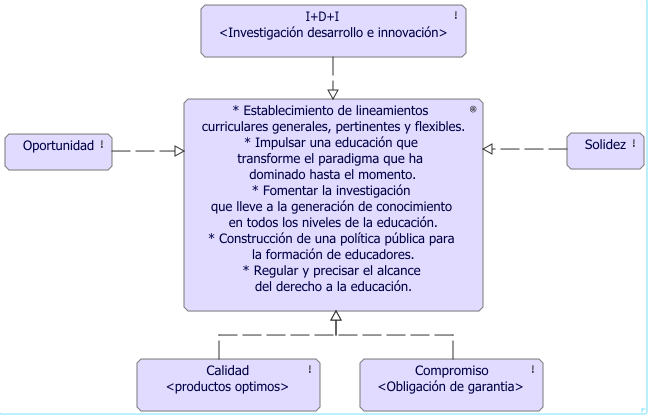
\includegraphics[width=1.0\linewidth]{imgs/motivacion/principios/principios}
	\caption{Caso Principios}
\end{figure}

Los principios que cualifican los objetivos corporativos relacionados con la calidad de la educación son aquellos que permiten el avance de forma asertada de lo que tiene que ver con el enfoque del fomento de investigaciones e impulso a la educación a un nivel mas alto, entre ellos tenemos la investigación desarrollo e innovación, calidad y compromiso.

%\newpage

\subsection{Caso  de Principios}
\begin{figure}[h]
	\centering
	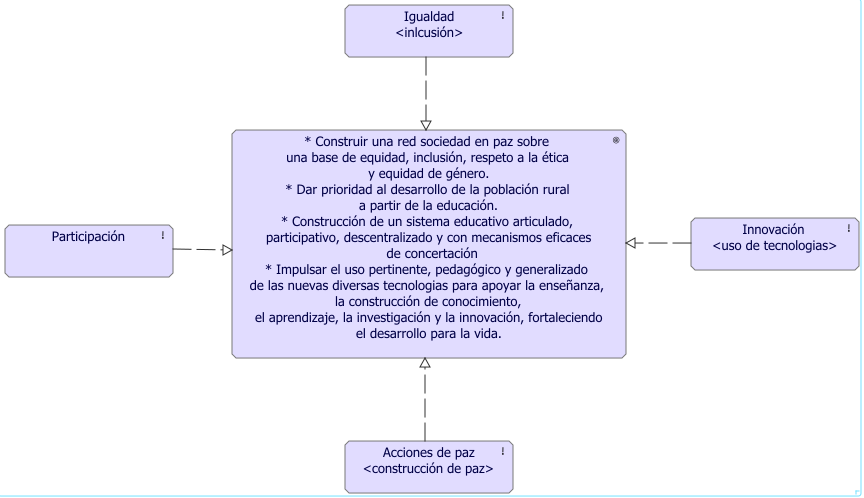
\includegraphics[width=1.0\linewidth]{imgs/motivacion/principios/principios_2}
	\caption{Caso Principios}
\end{figure}

Para construir la paz en nuestro país por medio de la educación que propone el MEN, se logra por medio de los principios que son base esencial para encontrar un equilibrio en la sociedad que potencie la entidad humana como se presentan en ek punto de vista de principios, entre ellos se tiene igualdad, participación, acciones de paz e innovación.
\section{Punto de Vista de Realización de Requerimientos}
El punto de vista de realización de requerimientos se basa en las necesidades que se requieren subsanar y que el sistema debe cumplir de manera satisfactoria, estos requerimientos, son los que definen las funciones que el sistema será capaz de realizar, describiendo las transformaciones que el sistema realiza sobre las entradas para producir salidas. Por decirlo de otra manera, estos requerimientos son los que posteriormente se van a transformar en algoritmos, es decir, en las funcionalidades del sistema.
Para la obtención de estos requerimientos, es necesario ademas de cumplir a detalle con una serie de pasos específicos, tener los objetivos, los cuales son el punto de partida para los requerimientos. Esta serie de pasos son: obtención, análisis, especificación, verificación y aceptación. Luego de esto, en la realización de requerimientos es en donde se especializan estos requerimientos.


\subsection{Modelo de Realización de Requerimientos}
\begin{figure}[h!]
	\centering
	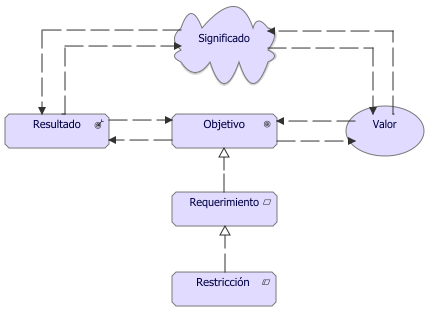
\includegraphics[width=1.0\linewidth]{imgs/modelo/RealRequerimientos}
	\caption{Modelo Realización de Requerimientos}
\end{figure}

El modelo del punto de vista de realización de requerimientos, como se ha evidenciado en los anteriores puntos de vista, parte de un objetivo central, del cual todo se desglosa, cuenta con diversas partes y herramientas como lo es el significado, valor, resultado y finalmente un requerimiento el cual se puede especializar cuantas veces lo permita.

%\newpage

\subsection{Caso  de Contribución de Objetivos}
\begin{figure}[h!]
	\centering
	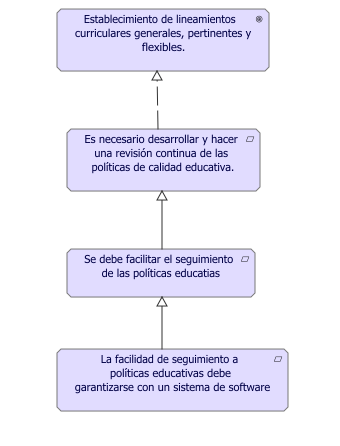
\includegraphics[width=0.6\linewidth]{imgs/motivacion/RealizaRequerimientos/realizaRequerimientos.pdf}
	\caption{Caso Realización de Requerimientos}
\end{figure}

En el proyecto planteado con el ministerio de educación nacional (MEN), y para la construcción del punto de vista de realización de requerimientos, en primer lugar se escogió un objetivo central del proyecto el cual es, Establecimiento de lineamientos curriculares generales, pertinentes y flexibles. A partir de este objetivo central, se dedujo un requerimiento como lo es: es necesario desarrollar y hacer una revisión continua de las políticas de calidad educativa, requerimiento del cual se puede especializar, tal como se hizo con el proyecto: se debe facilitar el seguimiento de las políticas educativas, y a su vez, esta especialización de requerimiento se pudo especializar una vez más: la facilidad de seguimiento a políticas educativas debe garantizarse con un sistema de software. Esta especialización de los requerimientos en la realización de los mismos, se puede hacer tantas veces como el mismo requerimiento lo permita.
\chapter{Motivacional}
\label{chap:Motivacional}
\section{Introducción}
Se han definido una serie de puntos de vista estándar para modelar los aspectos motivadores. Cada uno de estos puntos de vista presenta una perspectiva diferente para modelar la motivación que subyace en algunas arquitecturas empresariales y permite al modelador centrarse en ciertos aspectos. Por lo tanto, cada punto de vista considera sólo una selección de los elementos y relaciones que se han descrito en el capítulo 3.

Se distinguen los siguientes puntos de vista:

\begin{itemize}
	\item El punto de vista de los interesados se centra en la elaboración de modelos de los interesados, los factores determinantes, las evaluaciones de esos factores y los objetivos iniciales para abordar esos factores y evaluaciones.
	\item El punto de vista de la realización de los objetivos se centra en el perfeccionamiento de los objetivos iniciales de alto nivel para convertirlos en (sub)objetivos más concretos mediante la relación de agregación y, por último, en requisitos y limitaciones mediante la relación de realización.
	\item El punto de vista de la contribución al logro de objetivos se centra en la modelización y el análisis de las relaciones de influencia entre los objetivos (y los requisitos).
	\item El punto de vista de los principios se centra en la modelización de los principios pertinentes y las metas que motivan esos principios.
	\item El punto de vista de la realización de los requisitos se centra en la modelización de la realización de los requisitos y las limitaciones por medio de elementos básicos, como los agentes, los servicios, los procesos, los componentes de la aplicación, etc.
	\item El punto de vista de la motivación abarca todo el aspecto de la motivación y permite utilizar todos los elementos de motivación.
\end{itemize}

A continuación se describen por separado todos los puntos de vista. Para cada punto de vista, se indican sus elementos y relaciones, las directrices para su utilización, su objetivo y grupo destinatario. Además, la descripción de cada punto de vista contiene modelos de casos.
\newpage

\section{Metamodelo}
\begin{figure}[h!]
	\centering
	\includegraphics[width=1.0\linewidth]{imgs/meta/Motivacion}
	\caption{Metamodelo Motivacional}
\end{figure}

La principal jerarquía de los elementos de comportamiento y estructura del lenguaje ArchiMate se presenta en el metamodelo de la Figura 4.1. Define estos elementos de manera genérica e independiente de la capa. Observe que la mayoría de estos elementos (las cajas blancas) son elementos abstractos del meta modelo; es decir, no están instanciados en los modelos sino que sólo sirven para estructurar el meta modelo.  La notación presentada en este capítulo es, por lo tanto, la forma genérica en que se representan las especializaciones de estos elementos (es decir, los elementos de las diferentes capas de la arquitectura).  Los elementos concretos (las cajas grises), que pueden ser utilizados para modelar la Arquitectura de la Empresa a un nivel estratégico.\\ \\

Este fragmento genérico de metamodelo consiste en dos tipos principales de elementos: elementos de estructura ('sustantivos') y elementos de comportamiento ('verbos').

\newpage
\include{arquitectura/motivacion/implicados}
\include{arquitectura/motivacion/realizacionObj}
\include{arquitectura/motivacion/contribucionObj}
\include{arquitectura/motivacion/principios}
\include{arquitectura/motivacion/realizacionReq}
\include{arquitectura/motivacion/motivacion}







\chapter{Estrategia}
\section{Introduccion}
Además de los elementos de motivación descritos en el \autoref{chap:Motivacional}, el lenguaje también incluye una serie de elementos de estrategia, en particular la capacidad, los recursos y el curso de acción, como se muestra en la figura 5.1. Estos se definen como especializaciones de los elementos genéricos de comportamiento y estructura y se definen con más detalle en las siguientes secciones. \\

Para describir los aspectos estratégicos de la empresa se han definido los puntos de vista que se exponen a continuación. Cada uno de estos puntos de vista presenta una perspectiva diferente de la modelización de la dirección estratégica de alto nivel y de la composición de la empresa y permite a un modelador centrarse en determinados aspectos. Por lo tanto, cada punto de vista considera sólo una selección de los elementos y relaciones que se han descrito en las sección 3.3. Se distinguen los siguientes puntos de vista:

\begin{itemize}
	\item El punto de vista del mapa de capacidades proporciona una visión general de las capacidades de la empresa.
	\item El punto de vista de la realización de resultados describe la forma en que los resultados de alto nivel y orientados a los negocios se producen gracias a las capacidades y recursos de la empresa.
	\item El punto de vista del mapa de recursos proporciona una visión general estructurada de los recursos de la empresa.
\end{itemize}

\newpage

\section{Metamodelo}
\begin{figure}[h!]
	\centering
	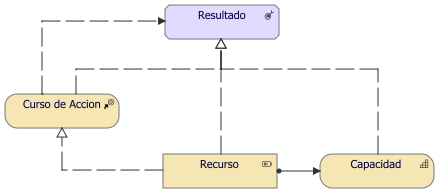
\includegraphics[width=0.9\linewidth]{imgs/meta/Estrategia}
	\caption{Metamodelo Motivacional}
\end{figure}

La figura 5.1 ofrece una visión general de los elementos de la estrategia y sus relaciones. Un recurso representa un activo que pertenece o está controlado por un individuo u organización.
Los recursos son un concepto central en el campo de la gestión estratégica, la economía, la informática, la gestión de carteras y más. A menudo se consideran, junto con las capacidades, como fuentes de ventaja competitiva para las organizaciones. Una capacidad representa una habilidad que posee un elemento de estructura activa, como una organización, una persona o un sistema.
En el ámbito de los negocios, el pensamiento y la planificación estratégicos proporcionan estrategias y objetivos de alto nivel que a menudo no se pueden aplicar directamente en la arquitectura de una organización. Un curso de acción es un enfoque o plan para configurar algunas capacidades y recursos de la empresa, emprendido para lograr un objetivo. Un curso de acción representa lo que una empresa ha decidido hacer. Los cursos de acción pueden ser categorizados como estrategias y tácticas. No es posible hacer una distinción estricta entre ambos, pero las estrategias tienden a ser a largo plazo y de alcance bastante amplio, mientras que las tácticas tienden a ser a corto plazo y de alcance más limitado.

\newpage
\chapter{Estrategia}
\section{Introduccion}
Además de los elementos de motivación descritos en el \autoref{chap:Motivacional}, el lenguaje también incluye una serie de elementos de estrategia, en particular la capacidad, los recursos y el curso de acción, como se muestra en la figura 5.1. Estos se definen como especializaciones de los elementos genéricos de comportamiento y estructura y se definen con más detalle en las siguientes secciones. \\

Para describir los aspectos estratégicos de la empresa se han definido los puntos de vista que se exponen a continuación. Cada uno de estos puntos de vista presenta una perspectiva diferente de la modelización de la dirección estratégica de alto nivel y de la composición de la empresa y permite a un modelador centrarse en determinados aspectos. Por lo tanto, cada punto de vista considera sólo una selección de los elementos y relaciones que se han descrito en las sección 3.3. Se distinguen los siguientes puntos de vista:

\begin{itemize}
	\item El punto de vista del mapa de capacidades proporciona una visión general de las capacidades de la empresa.
	\item El punto de vista de la realización de resultados describe la forma en que los resultados de alto nivel y orientados a los negocios se producen gracias a las capacidades y recursos de la empresa.
	\item El punto de vista del mapa de recursos proporciona una visión general estructurada de los recursos de la empresa.
\end{itemize}

\newpage

\section{Metamodelo}
\begin{figure}[h!]
	\centering
	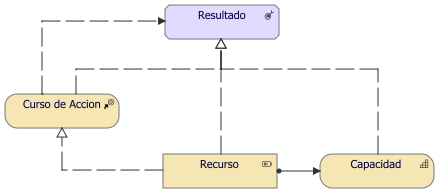
\includegraphics[width=0.9\linewidth]{imgs/meta/Estrategia}
	\caption{Metamodelo Motivacional}
\end{figure}

La figura 5.1 ofrece una visión general de los elementos de la estrategia y sus relaciones. Un recurso representa un activo que pertenece o está controlado por un individuo u organización.
Los recursos son un concepto central en el campo de la gestión estratégica, la economía, la informática, la gestión de carteras y más. A menudo se consideran, junto con las capacidades, como fuentes de ventaja competitiva para las organizaciones. Una capacidad representa una habilidad que posee un elemento de estructura activa, como una organización, una persona o un sistema.
En el ámbito de los negocios, el pensamiento y la planificación estratégicos proporcionan estrategias y objetivos de alto nivel que a menudo no se pueden aplicar directamente en la arquitectura de una organización. Un curso de acción es un enfoque o plan para configurar algunas capacidades y recursos de la empresa, emprendido para lograr un objetivo. Un curso de acción representa lo que una empresa ha decidido hacer. Los cursos de acción pueden ser categorizados como estrategias y tácticas. No es posible hacer una distinción estricta entre ambos, pero las estrategias tienden a ser a largo plazo y de alcance bastante amplio, mientras que las tácticas tienden a ser a corto plazo y de alcance más limitado.

\newpage
\include{arquitectura/estrategia/estrategia}

\newpage
\include{arquitectura/estrategia/capacidad}


\newpage
\include{arquitectura/estrategia/resultado}

\newpage
\include{arquitectura/estrategia/recurso}



\newpage
\section{Punto de Vista de Mapa de Capacidad}

El punto de vista del mapa de capacidades permite al arquitecto de la empresa crear una visión general estructurada de las capacidades de la empresa. Un mapa de capacidad típicamente muestra dos o tres niveles de capacidades en toda la empresa. Puede, por ejemplo, utilizarse como mapa de calor para identificar áreas de inversión. En algunos casos, un mapa de capacidades también puede mostrar los resultados específicos que ofrecen esas capacidades.

\subsection{Modelo de Mapa de Capacidad}
\begin{figure}[h!]
	\centering
	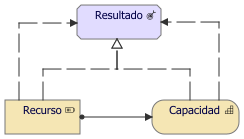
\includegraphics[width=.5\linewidth]{imgs/caso/MapaCapacidad}
	\caption{Modelo Mapa de Capacidad}
\end{figure}

En sínstesis, un recurso es un activo que es propiedad o está controlado por un individuo u organización. Por otra parte, una capacidad es una habilidad que posee un elemento de estructura activa, como una organización, una persona o un sistema. Y, finalmente, un curso de acción es un enfoque o plan para configurar algunas capacidades y recursos de la empresa, dispustos para la consecusión de un objetivo. \\

Aumentar el beneficio es un objetivo que puede descomponerse en varios otros objetivos: Disminuir los costos y aumentar los ingresos. El primero está relacionado con la estrategia de Operación Excelencia de la empresa, modelada como un curso de acción. Estos resultan en dos resultados: Disminución de los costos y pérdida de clientes, que influyen en los objetivos de manera positiva y negativa. Esto muestra una importante diferencia entre los objetivos y los resultados: no todos los resultados conducen a los resultados previstos.
Los cursos de acción se realizan por una serie de capacidades: Gestión y operaciones de TI y gestión de productos, y los recursos apropiados Recursos humanos y recursos de TI se asignan a las primeras.

\newpage

\subsection{Caso de Mapa de Capacidad}

\subsubsection{Resutlado 1: Mejores Investigadores e Investigaciones}

\begin{figure}[h!]
	\centering
	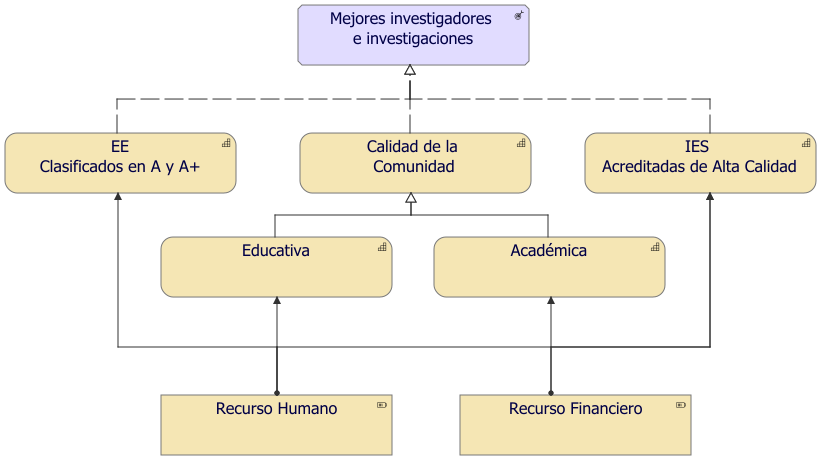
\includegraphics[width=1\linewidth]{imgs/modelo/estrategia/capacidad/1.pdf}
	\caption{Caso Mapa de Capacidad}
\end{figure}

Para dar alcance al resultado de obtener mejores investigadores y mejores investigaciones, el MEN como estructura activa se basa en las habilidades inmersas tanto en los Establecimientos Educativos de calificación A y A+ \footnote{\url{https://www.icfes.gov.co/documents/20143/193495/Clasificacion+de+establecimientos+y+sedes+Saber+11.pdf/2f177381-3c38-6b20-f5da-272dba42b412}}, los cuales representan la mayoría de los planteles registrados, así como las habilidades al interior de sus Instituciones de Educación Superior acreditadas de alta calidad. \\

No obstante, estas habilidades se encuentran arraigadas a la capacidad provista por la calidad de la comunidad, educativa y académica respectivamente. A saber, el activo más importante del MEN, el recurso humano; y que, junto al recurso financiero, conforman el punto de partida para el curso de acción de la organización.

\clearpage
\subsubsection{Resutlado 2: Generación de Estudiantes de Alta Calidad}

\begin{figure}[h!]
	\centering
	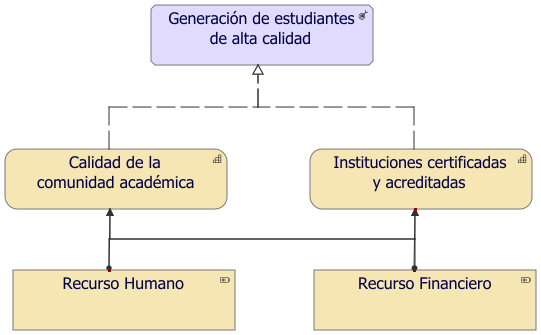
\includegraphics[width=.7\linewidth]{imgs/modelo/estrategia/capacidad/2.pdf}
	\caption{Caso Mapa de Capacidad}
\end{figure}

En en el marco de la \textbf{generación de estudiantes} de alta calidad, el MEN dispone de dos capacidades como lo son la calidad de la comunidad académica e instituciones certificadas y acreditadas que garantizan el desarrollo de procesos con altos estándares de calidad. Las cuales, junto con los recursos humano y financiero, se encuntran configurados dentro del curso de acción para la consecusión de dicho objetivo.


\newpage
\section{Punto de Vista de Realización de resultado}

El punto de vista de la realización de resultados se utiliza para mostrar cómo las capacidades y los elementos básicos subyacentes producen resultados de más alto nivel orientados al negocio.

\subsection{Modelo de Realización de resultado}
\begin{figure}[h!]
	\centering
	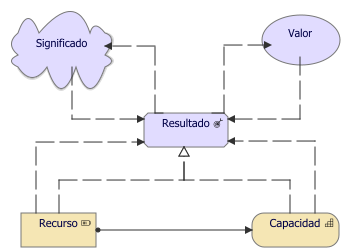
\includegraphics[width=.5\linewidth]{imgs/caso/RealResultado.pdf}
	\caption{Modelo Realización de resultado}
\end{figure}

El punto de vista de la realización de resultados describe cómo las capacidades y los recursos de la empresa producen resultados de alto nivel orientados al negocio.

\newpage

\subsection{Caso de Realización de resultado}

\subsubsection{Resultado 1: Mejores Investigadores e Investigaciones}

\begin{figure}[h!]
	\centering
	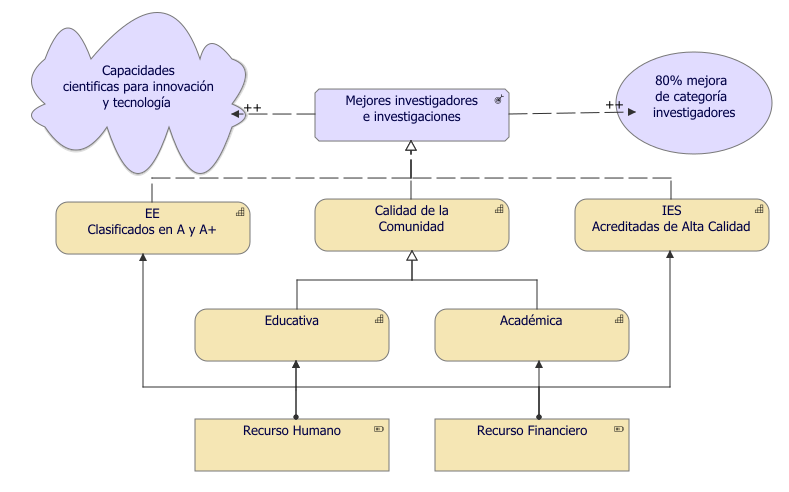
\includegraphics[width=.8\linewidth]{imgs/modelo/estrategia/resultado/resultado_2.pdf}
	\caption{Caso Realización de resultado}
\end{figure}

Para el caso de resultado de \textbf{Mejores Investigadores e Investigaciones} se busca promover nuevas capacidades científicas que fomenten la innovación y la tecnología gracias comunidad de calidad, de las IES acreditadas de alta calidad. Se pretende alcanzar el 80 por ciento en subir de categoría por parte de los investigadores.


\clearpage
\subsubsection{Resultado 2: Generación de Estudiantes de Alta Calidad}

\begin{figure}[h!]
	\centering
	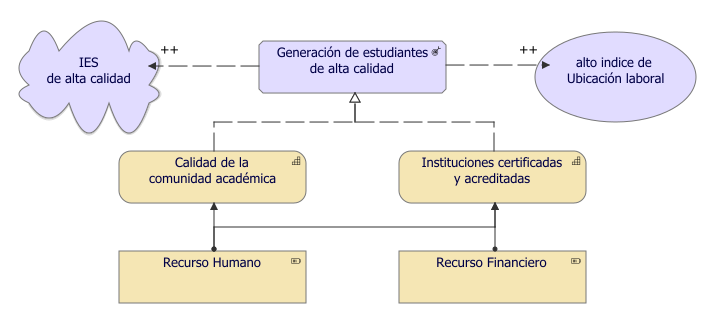
\includegraphics[width=.8\linewidth]{imgs/modelo/estrategia/resultado/resultado.pdf}
	\caption{Caso Realización de resultado}
\end{figure}

El resultado de \textbf{generación de estudiantes de alta calidad} proporciona un significado de grandes expectativas para el MEN, puesto que este resultado da como garantía Instituciones de Educación Superior(IES) de alta calidad promoviendo la capacidad de calidad en la comunidad académica ademas de instituciones certificadas y acreditadas.

\newpage
\section{Punto de Vista de Mapa de Recurso}

El punto de vista del mapa de recursos permite al arquitecto comercial crear una descripción general estructurada de los recursos de la empresa. Un mapa de recursos generalmente muestra dos o tres niveles de recursos en toda la empresa. Puede, por ejemplo, utilizarse como mapa de calor para identificar áreas de inversión. En algunos casos, un mapa de recursos también puede mostrar relaciones entre los recursos y las capacidades a las que están asignados.

\subsection{Modelo de Mapa de Recurso}
\begin{figure}[h!]
	\centering
	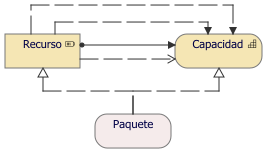
\includegraphics[width=.5\linewidth]{imgs/caso/MapaRecurso.pdf}
	\caption{Modelo Mapa de Recurso}
\end{figure}

El punto de vista del mapa de recursos proporciona una descripción estructurada de los recursos de la empresa.

\newpage

\subsection{Caso de Mapa de Recurso}

\subsubsection{Resultado 1: Mejores Investigadores e Investigaciones}

\begin{figure}[h!]
	\centering
	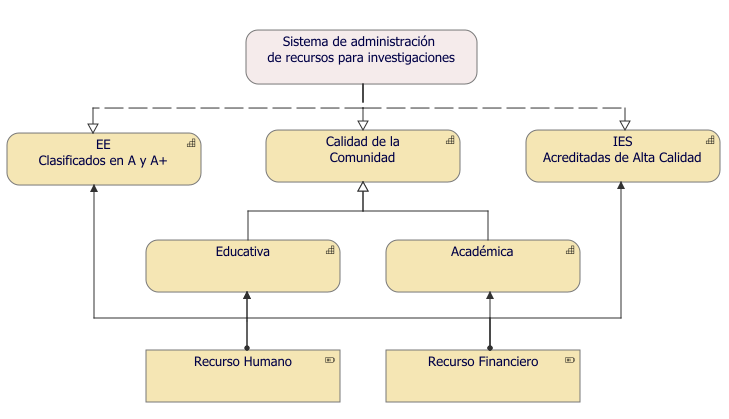
\includegraphics[width=1\linewidth]{imgs/modelo/estrategia/mapa/mapa_recurso.pdf}
	\caption{Caso Mapa de Recurso}
\end{figure}

Para dar alcance a las capacidades de calidad de la comunidad, IES Acreditadas de Alta Calidad y EE Clasificados en A y A+ basadas en habilidades dadas por el resultado de Mejores Investigadores e Investigaciones, se pretende construir un sistema que administre de manera optima los recursos para realizar nuevas investigaciones dando lugar a un crecimiento exponencial de nuevos investigadores.

\clearpage
\subsubsection{Resultado 2: Generación de Estudiantes de Alta Calidad}

\begin{figure}[h!]
	\centering
	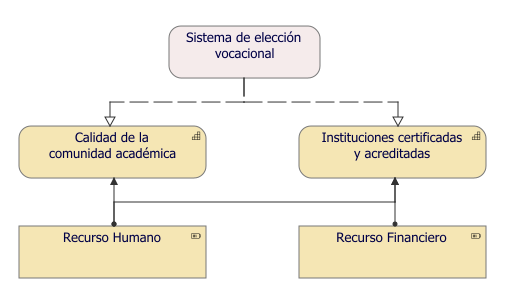
\includegraphics[width=.8\linewidth]{imgs/modelo/estrategia/mapa/mapa_recurso_2.pdf}
	\caption{Caso Mapa de Recurso}
\end{figure}

Para garantizar la generación de estudiantes de calidad es necesario implantar nuevos sistemas que ayudan a elegir de mejor manera la vocación que tendrán en el futuro los estudiantes. Buscando así que el estudiante se acerque a las diferentes carreras o áreas del conocimiento sin sentir presión por parte de ningún ente, que aquella vocación escogida por el estudiante sea totalmente de su agrado y gusto; formando estudiantes que lleven la educación de calidad no por obligación sino por interés propio.



\subsection{Negocio}

La Capa de Negocios se utiliza típicamente (en conjunto con los elementos de estrategia) para modelar la arquitectura de negocios de una empresa, definida por el marco del TOGAF como una descripción de la estructura e interacción entre la estrategia de negocios, la organización, las funciones, los procesos de negocios y las necesidades de información.

\subsubsection{Elementos de la Estructura}
\begin{table}[H]
	\centering
	\begin{tabular}{| m{3cm} | m{7cm} | m{3.8cm} |}
		\hline
		\textbf{Concepto}           & \textbf{Definición} & \textbf{Notación} \\ \hline
		
		Actor de Negocios        & Una entidad organizacional que es capaz de ejecutar un comportamiento.                                                                                                              &\vspace{1.52mm}\includegraphics[width=40mm, height=10mm]{imgs/conceptos/negocio/Business_actor.pdf}    \\ \hline
		
		Rol de Negocios          & La responsabilidad de tener un comportamiento especifico, ante el cual un actor puede ser asignado.                                                                                 &\vspace{1.52mm}\includegraphics[width=40mm, height=10mm ]{imgs/conceptos/negocio/Business_role.pdf}         \\ \hline
		
		Colaboración de Negocios & Un agregado de dos o más roles de negocios que trabajan juntos para tener un comportamiento colectivo.                                                                             
		&\vspace{1.52mm} \includegraphics[width=40mm,height=10mm]{imgs/conceptos/negocio/Business_colaboration.pdf}             \\ \hline
		
		Interfaz de Negocios     & Un punto de acceso donde un servicio comercial está disponible para su entorno.                                                                                                     
		&\vspace{1.52mm}\includegraphics[width=40mm,height=10mm]{imgs/conceptos/negocio/Business_Interface.pdf}  \\ \hline
		
		Ubicación                & Un punto conceptual en el espacio.                                                                                     
		&\vspace{1.52mm}\includegraphics[width=40mm, height=10mm]{imgs/conceptos/negocio/Location.pdf}           \\ \hline
		
		Objeto de Negocios       & Un elemento pasivo que tiene relevancia desde una perspectiva de negocios.                                                                                                         
		&\vspace{1.52mm}\includegraphics[width=40mm, height=10mm]{imgs/conceptos/negocio/Business_Object.pdf}   \\ \hline
		
		Proceso de Negocios      & Un elemento de comportamiento que agrupa el comportamiento basado en un orden de actividades. Es destinado a producir un  conjunto definido de productos o servicios comerciales.
		&\vspace{1.52mm} \includegraphics[width=40mm, height=10mm]{imgs/conceptos/negocio/Business_proces.pdf}            \\ \hline
		
		Función de Negocios      & Un elemento de comportamiento que agrupa el comportamiento basado en un conjunto de criterios elegidos (típicamente recursos comerciales requeridos y / o competencias).        &\vspace{1.52mm}\includegraphics[width=40mm, height=10mm]{imgs/conceptos/negocio/Business_function.pdf}            \\ \hline
		
		Interacción de Negocios  & Un elemento de comportamiento que describe la conducta de una colaboración empresarial.                                                                                             
		&\vspace{1.52mm} \includegraphics[width=40mm,height=10mm]{imgs/conceptos/negocio/Business_interaction.pdf}            \\ \hline
		
		Evento de Negocios       & Algo que sucede (internamente o externamente) e influye en el  comportamiento.                                                                                                       
		&\vspace{1.52mm} \includegraphics[width=40mm, height=10mm]{imgs/conceptos/negocio/Business_event.pdf}  \\ \hline
		
	\end{tabular}
\end{table}

\newpage
\begin{table}[H]
	\centering
	\begin{tabular}{| m{3cm} | m{7cm} | m{3.8cm} |}
		\hline
		\textbf{Concepto}           & \textbf{Definición} & \textbf{Notación} \\ \hline
		
		Servicio de Negocios     & Un servicio que satisface una necesidad comercial de un cliente (interno o externo al organización).        &\vspace{2mm}\includegraphics[width=40mm, height=8mm]{imgs/conceptos/negocio/Business_service.pdf}  \\ \hline
		
		Representación           & Una forma perceptible de la información llevado por un objeto de negocios.                                                                                                           &\vspace{1.52mm}  \includegraphics[width=40mm, height=10mm]{imgs/conceptos/negocio/Representation.pdf}            \\ \hline
		Significado              & El conocimiento o experiencia presente en un objeto de negocios o su representación, dado un contexto particular.                                                                   &\vspace{1.52mm}\includegraphics[width=40mm, height=8mm]{imgs/conceptos/negocio/Meaning.pdf}           \\ \hline
		
		Valor                    & El valor relativo, la utilidad o la importanciade un servicio o producto comercial.                                                                                                  
		&\vspace{1.52mm}\includegraphics[width=40mm, height=10mm]{imgs/conceptos/negocio/Value.pdf}        \\ \hline
		
		Producto                 & Una colección coherente de servicios, acompañado de un contrato / conjunto de acuerdos, que se ofrece en su conjunto para (internos o externos) clientes.                           &\vspace{1.52mm}\includegraphics[width=40mm, height=10mm]{imgs/conceptos/negocio/Product.pdf}         \\ \hline
		
		Contrato                 & Una especificación formal o informal de acuerdo que especifica los derechos y obligaciones asociadas con un producto.                                                                 &\vspace{1.52mm}\includegraphics[width=40mm, height=10mm]{imgs/conceptos/negocio/Contract.pdf}       \\ \hline
		
	\end{tabular}
\end{table}

\chapter{Aplicación}
\section{Introducción}
La Capa de Aplicación muestra los servicios de aplicación que apoyan el negocio, y las aplicaciones que los realizan.
El principal elemento de estructura activa de la Capa de Aplicación es el componente de aplicación. Este elemento se utiliza para modelar cualquier entidad estructural en la Capa de Aplicación: no sólo los componentes de software (reutilizables) que pueden formar parte de una o más aplicaciones, sino también las aplicaciones de software completas, las subaplicaciones o los sistemas de información. Aunque es muy similar al UML componente, el elemento componente de la aplicación ArchiMate modela estrictamente el aspecto estructural de una aplicación; su comportamiento está modelado por una relación explícita con el elemento de comportamiento.
También en la arquitectura de aplicación, las interrelaciones de los componentes son un ingrediente esencial. Por lo tanto, también introducimos aquí el elemento de colaboración de la aplicación, definido como un colectivo de componentes de aplicación que realizan interacciones de aplicación. El elemento es muy similar a la colaboración como se define en el estándar UML.
En el sentido puramente estructural, una interfaz de aplicación es el canal (lógico) a través del cual se puede acceder a los servicios de un componente. En un sentido más amplio (tal como se utiliza, entre otros, en la definición de UML), una interfaz de aplicación define algunas características de comportamiento elementales: define el conjunto de operaciones y eventos que proporciona el componente, o los que se requieren del entorno. Así, se utiliza para describir la funcionalidad de un componente. El elemento de interfaz de aplicación puede utilizarse para modelar tanto las interfaces de aplicación a aplicación, que ofrecen servicios de aplicación internos, como las interfaces de aplicación a empresa (y/o interfaces de usuario), que ofrecen servicios de aplicación externos.

\section{Metamodelo}
\begin{figure}[h!]
	\centering
	\includegraphics[width=0.9\linewidth]{imgs/meta/Aplicacion}
	\caption{Metamodelo Aplicación}
\end{figure}

La figura 7.1 brinda una visión general de los elementos de la capa de aplicación y sus relaciones. Siempre que sea aplicable, la guía se ha extraído de la analogía con la Capa de Aplicación. La Capa de Aplicación se utiliza típicamente para modelar las arquitecturas de los sistemas de información de la empresa, incluida la arquitectura de aplicación que, como se define en el marco del TOGAF, describe la estructura e interacción de las aplicaciones. Un componente de aplicación representa una encapsulación de la funcionalidad de la aplicación alineada con la estructura de implementación, que es modular y reemplazable. Encapsula su comportamiento y datos, expone los servicios y los hace disponibles a través de interfaces.

\newpage
\chapter{Comportamiento}
\section{Introduccion}
contenido...

\newpage
\section{Punto de Vista de Cooperación de Actor}


\subsection{Modelo de Cooperación de Actor}
\begin{figure}[h!]
	\centering
	\includegraphics[width=.6\linewidth]{imgs/modelo/CoopActor.pdf}
	\caption{Modelo Cooperacion de Actor}
\end{figure}

El punto de vista de cooperación de actor establece las colaboraciones que existen internamente y externamente sobre un actor o rol de la organización con el fin de mostrar de qué manera interactuan e interfiere con el actor en cuestión. Por medio de interfaces  que comunican los entes del exterior y el interior de la organización con el actor o rol.

\newpage
\subsection{Caso  de Cooperación de Actor}
\begin{figure}[h!]
	\centering
	\includegraphics[width=.8\linewidth]{imgs/caso/negocio/coperacion_actor.pdf}
	\caption{Caso Cooperacion de Actor}
\end{figure}

Para nuestro objeto de estudio en relación al punto de vista de colaboración de actor tenemos como actor principal a los estudiantes aquellos que colaboran en la comunidad académica y hacen parte de las IES y EE que son regidas por el Ministerio de Educación. Por otro lado tenemos el rol de educador que hace parte de la comunidad y que puede ayudar a guiar en parte la vocación que construirá en un futuro el estudiante. Los estudiantes contribuirán en la sociedad gracias a su perfil que se ha formado durante sus años de estudio y que permitirán a las empresas apoderarse de estos individuos y así lograr mejores avances que colaboren en su entidad y por tanto a la sociedad misma.

\newpage
\section{Punto de Vista Estructura de Información}
Una estructura de información es una estructura jerárquica centrada en el producto que organiza la información relacionada con un producto o biblioteca. Dentro de una estructura de información, los subgrupos de información denominados grupos de información organizan el contenido. Estos objetos de contenido se denominan elementos de información. Los criterios de filtro ofrecen la posibilidad de identificar y administrar la información asociada a las variaciones del producto. Las estructuras de información se pueden filtrar para mostrar componentes opcionales o artículos con valores de atributo específicos. Los objetos se muestran en la estructura según el filtro de la estructura actualmente activo. Se pueden editar los filtros y renovar la estructura para mostrar los objetos que cumplen con los nuevos criterios de filtro. Las estructuras de información se pueden comparar para determinar el impacto de los cambios en el producto. La estructura de información que se encuentra actualmente en producción se puede comparar con una nueva estructura de información bajo desarrollo para revelar el impacto de los cambios propuestos. Las relaciones con la información de producto de soporte permiten determinar la cantidad y el ámbito del trabajo que se va a hacer.

\subsection{Modelo de Estructura de Información}
\begin{figure}[h!]
	\centering
	\includegraphics[width=.62\linewidth]{imgs/modelo/EstrInformacion}
	\caption{Modelo Estructura de Información}
\end{figure}

Esta quinta sección de puntos de vista llamada tecnología en la cual se involucra todo lo concerniente a la parte tecnológica, su uso, la implementación y el despliegue, la parte física, las capas, el servicio y la estructura de la información del proyecto, este último punto de vista de la estructura de información está compuesto por cinco elementos principalmente, tal y como se muestra en el diagrama anterior del modelo. Estos elementos son: como principal, está el objeto y el objeto secundario, luego se deriva en una representación y significado del mismo y por la parte de los objetos se desprende un artefacto por medio de una realización. 


\subsection{Caso  de Estructura de Información}
\begin{figure}[h!]
	\centering
	\includegraphics[width=.8\linewidth]{imgs/caso/estructuraInformaci}
	\caption{Caso Estructura de Información}
\end{figure}

El punto de vista de la estructura de la información es comparable a los modelos de información tradicionales creados en el desarrollo de casi cualquier sistema de información. Muestra la estructura de la información utilizada en la empresa o en un proceso de negocio o aplicación específicos, en términos de tipos de datos o estructuras de clases (orientadas a objetos). Además, puede mostrar cómo la información a nivel empresarial se representa en el nivel de la aplicación en la forma de las estructuras de datos que se utilizan allí, y cómo se asignan luego a la infraestructura tecnológica subyacente, destacando que es un enfoque de muy alto nivel hacia por ejemplo, por medio de un esquema de base de datos, tal y como se realizó para el proyecto Tu-Perfil en donde se tiene el objeto de negocio llamado Perfil Web y una serie de elementos o entidades importantes a tener en cuenta para modelar como los perfiles que tiene un perfil para una profesión y lógicamente el estudiante a perfilar, sin dejar de lado la parte del juego o Game que realiza la función de brochure para la base de datos.

\clearpage

\newpage
\section{Punto de Vista de Uso de Tecnología}

El punto de vista de la utilización de la tecnología muestra cómo las aplicaciones son apoyadas por la tecnología de software y hardware: los servicios tecnológicos son suministrados por los dispositivos; el software y las redes del sistema son suministrados a las aplicaciones. Este punto de vista desempeña un papel importante en el análisis del rendimiento y la escalabilidad, ya que relaciona la infraestructura física con el mundo lógico de las aplicaciones. Es muy útil para determinar los requisitos de rendimiento y calidad de la infraestructura en función de las exigencias de las diversas aplicaciones que la utilizan.

\subsection{Modelo de Uso de la Tecnología}
\begin{figure}[h!]
	\centering
	\includegraphics[width=.8\linewidth]{imgs/modelo/UsoTecnologia.pdf}
	\caption{Modelo Uso de Tecnología}
\end{figure}

Una función tecnológica describe el comportamiento interno de un nodo; para el usuario de un nodo que realiza una función tecnológica, esta función es invisible. Si su comportamiento es expuesto externamente, esto se hace a través de uno o más servicios tecnológicos. Una función tecnológica se abstrae de la forma en que se implementa. Sólo se especifica el comportamiento necesario. Una función de tecnología puede realizar servicios de tecnología. Los servicios tecnológicos de otras funciones tecnológicas pueden servir a las funciones tecnológicas. Una función tecnológica puede acceder a los objetos tecnológicos. Se puede asignar un nodo a una función tecnológica (lo que significa que el nodo realiza la función tecnológica). El nombre de una función tecnológica debe ser preferentemente un verbo sustantivado.

%\newpage

\subsection{Caso  de  Uso de la Tecnología}
\begin{figure}[h!]
	\centering
	\includegraphics[width=.8\linewidth]{imgs/puntos_vista/tecnologia/uso.pdf}
	\caption{Caso de Uso de la Tecnología}
\end{figure}

Para nuestro caso, en el servidor de aplicaciones vamos a desplegar los componentes descritos en la capa de aplicación, a saber, el componente orquestador Tu-Perfil, los componentes pertenecientes al core de la aplicación, como lo son el componente Profesión, Juego, y Estudiante, además del componente del front, GUI. Por otra parte, se especifican dos componentes externos, el primero de ellos denominado Games, el cual, nos permite integrar juegos online que proporcionan datos sobre las partidas de los juegos y sus correspondientes puntajes en cada una de las modalidades o categorías para ser enviadas y analizadas para el perfilamiento del estudiante. Luego, se especifica el componente Empleabilidad, que nos brinda una estadística sobre las profesiones con mayor demanda en periodos de tiempo ajustables mediante el uso de diferentes datasets. 

\subsection{Punto de Vista de la Tecnología}
El punto de vista de infraestructura general, trata acerca del hardware y la infraestructura de comunicación que soporta la capa de aplicación. Esta capa ofrece servicios de infraestructura requeridos para desplegar las aplicaciones realizadas en los ordenadores y los sistemas de
hardware y software.



\subsubsection{Punto de vista de uso de infraestructura}

El punto de vista de uso de infraestructura muestra como las aplicaciones son soportadas por la infraestructura de software y hardware: los servicios de infraestructura son entregados por los dispositivos, los sistemas de software y redes son entregados a las aplicaciones. Este
punto de vista juega un rol importante en el análisis del rendimiento y la escalabilidad y puede ser usado para determinar requerimientos de rendimiento y calidad en la infraestructura basado en las demandas de las aplicaciones que la usan.
\newpage

\begin{figure}[h]
	\centering
	\fcolorbox{black}{white}{
		\includegraphics[width=0.5\linewidth]{imgs/puntos_vista/tecnologia/MMDUDI.jpg}}
	\caption{Metamodelo de uso de infraestructura}
\end{figure}

\subsubsection{Modelo de uso de infraestructura}

En este punto de vista se identifican los servicios de infraestructura principales que corresponden al servicio de notificaciones, generar reportes, establecer tiempos de acceso a la
aplicación, y gestionar los usuarios. Cada uno de los servicios de infraestructura entrega configuración y la funcionalidad requerida hacia los componentes de aplicación.


\begin{figure}[h]
	\centering
	\fcolorbox{black}{white}{
		\includegraphics[width=0.5\linewidth]{imgs/puntos_vista/tecnologia/MDUDI.jpg}}
	\caption{Modelo de uso de infraestructura}
\end{figure}



\subsubsection{ Punto de vista de Implementación y despliegue}
El punto de vista de implementación y despliegue muestra como uno o más aplicaciones son realizadas sobre la infraestructura. Esto implica el mapeo de aplicaciones (lógicas) y componentes en artefactos (físicos). Esta vista juega un papel importante en el análisis del rendimiento y la escalabilidad debido a la relación entre la infraestructura y el mundo lógico de las aplicaciones.


\begin{figure}[h]
	\centering
	\fcolorbox{black}{white}{
		\includegraphics[width=0.5\linewidth]{imgs/puntos_vista/tecnologia/MMDIYD.jpg}}
	\caption{Metamodelo de implementación y despliegue}
\end{figure}

\subsubsection{Modelo de implementación y despliegue}

En este punto de vista, se muestra como todos los componentes son realizados por el nodo de servidor de aplicaciones, el componente de comunicación va a ser realizado por el nodo servidor de aplicaciones y tiene una relación de asociación con el nodo servidor de e-mail que
proveerá las configuraciones de software específico para el envío de notificaciones, resultados e información sobre el proceso.

\begin{figure}[h]
	\centering
	\fcolorbox{black}{white}{
		\includegraphics[width=0.5\linewidth]{imgs/puntos_vista/tecnologia/MDIYD.jpg}}
	\caption{Modelo de implementación y despliegue}
\end{figure}



\begin{table}[h]
	\begin{center}
		\begin{tabular}{ | m{7em} | m{8cm}|  } 
			\hline
			Interesados & Arquitectos de infraestructura, gerentes operativos 
			\\
			\hline
			Preocupaciones & Estabilidad, seguridad, dependencias, costos de la infraestructura
			\\
			\hline
			Propósito & Diseñar
			\\
			\hline
			Alcance & Una capa / aspecto múltiple
			\\
			\hline
		\end{tabular}
		\caption{Punto de Vista Tecnología}
		\label{tab:concepts}
	\end{center}
\end{table}

\textbf{Elementos que participan: }
\begin{itemize}
	\item Ubicación
	\item Nodo
	\item Colaboración tecnológica
	\item Dispositivo
	\item Software del sistema
	\item Interfaz tecnológica
	\item Red de comunicacion
	\item Camino
	\item Proceso tecnológico / función / interacción
	\item Servicio de tecnología
	\item Evento tecnológico
	\item Artefacto
\end{itemize}

\section{Punto de Vista Físico}
\subsection{Modelo Físico}
\begin{figure}[h!]
	\centering
	\includegraphics[width=.9\linewidth]{imgs/modelo/Fisico}
	\caption{Modelo Físico}
\end{figure}

El punto de vista físico es importante para los proyectos a realizar a escala industrial, no por el hecho de que sea fundamental para la construcción del proyecto sino más que todo es para su puesta en marcha. Como es bien sabido, todos los proyectos se realizan con alguna razón de ser, generalmente para cumplir una necesidad y/o ayudar a la comunidad con una función en específico, teniendo en cuenta esto, para la implementación y puesta en marcha del proyecto, es necesario tener en cuenta el punto de vista físico si el proyecto  así lo requiere.

Para el caso del proyecto Tu-Perfil, este no requiere un punto de vista físico como tal, puesto que no cuenta con los requisitos para que este exista, no se va a construir a gran escala o a escala industrial y todos los servicios que brinda este proyecto son digitales, por lo tanto aparte de las herramientas de computación y servidores no se requiere más indumentaria física.

\clearpage


\section{Relaciones}

el lenguaje ArchiMate define un conjunto básico de relaciones genéricas, cada una de las cuales puede conectar un conjunto predefinido de conceptos de origen y destino (en la mayoría de los casos elementos, pero en unos pocos casos también otras relaciones).  Muchas de estas relaciones están "sobrecargadas"; es decir, su significado exacto difiere según los conceptos de origen y destino que conectan, y se clasifican de la siguiente manera:
\begin{itemize}
	\item Relaciones estructurales, que modelan la construcción o composición estática de conceptos del mismo o diferentes tipos.
	\item Relaciones de dependencia, que modelan cómo se utilizan los elementos para apoyar otros elementos.
	\item Las relaciones dinámicas, que se utilizan para modelar las dependencias de comportamiento entre los elementos.
	\item Otras relaciones, que no entran en ninguna de las categorías anteriores.
\end{itemize}

\subsection{Relaciones Estructurales}

Las relaciones estructurales representan la coherencia "estática" dentro de una arquitectura.  El concepto de composición (el lado "de" de la relación) es siempre un elemento; el concepto de composición (el lado "de" de la relación) puede en algunos casos ser también otra relación.

\begin{table}[h!]
	\subsubsection{Elementos}
	\begin{center}
		\begin{tabular}{| l | l | r |}
			\hline
			Concepto & Descripción & Representación \\ \hline
			
			Agregación 
			&
			\begin{tabular}[l]{@{}l@{}}
				Indica que un elemento consiste en \\
				uno u otros conceptos más.
			\end{tabular}
			& \includegraphics[width=0.4\linewidth]{imgs/relaciones/agregacion}
			\\\hline
			
			Composición
			& 
			\begin{tabular}[l]{@{}l@{}}
				Indica que un elemento consiste en \\
				uno u otros conceptos más.
			\end{tabular}
			& \includegraphics[width=0.4\linewidth]{imgs/relaciones/composicion}
			\\\hline
			
			Asignación
			& 
			\begin{tabular}[l]{@{}l@{}}
				Expresa la asignación de \\
				responsabilidad, la ejecución \\
				de la conducta, o la ejecución.
			\end{tabular}
			& \includegraphics[width=0.4\linewidth]{imgs/relaciones/asignacion}
			\\\hline
			
			Realización
			& 
			\begin{tabular}[l]{@{}l@{}}
				Indica que una entidad desempeña \\
				un papel fundamental en la creación,\\
				el logro, el sustento o el \\
				funcionamiento de una entidad más \\
				abstracta.
			\end{tabular}
			& \includegraphics[width=0.4\linewidth]{imgs/relaciones/realizacion}
			\\\hline
			
		\end{tabular}
		\caption{Relaciones estructurales}
		\label{tab:estructurales}
	\end{center}
\end{table}

\subsection{Relaciones de Dependencia}

Las relaciones de dependencia describen la forma en que los elementos apoyan o son utilizados por otros elementos.  Se distinguen tres tipos de relaciones de dependencia:
\begin{itemize}
	\item La relación de servicio representa una dependencia de control, denotada por una línea sólida.
	\item La relación de acceso representa una dependencia de datos, denotada por una línea discontinua.
	\item La relación de influencia es el tipo de dependencia más débil, utilizada para modelar cómo los elementos de motivación son influenciados por otros elementos.
\end{itemize}
Obsérvese que, aunque la notación de estas relaciones se asemeja a la notación de la relación de dependencia en UML, estas relaciones tienen significados distintos en la notación ArchiMate y (normalmente) apuntan en la dirección opuesta.

\begin{table}[h!]
	\subsubsection{Elementos}
	\begin{center}
		\begin{tabular}{| c | l | l |}
			\hline
			Concepto & Descripción & Representación \\ \hline
			
			Sirve 
			&
			\begin{tabular}{m{12em}}
				Modela que un elemento proporciona
				su funcionalidad a otro elemento.
			\end{tabular}
			& \includegraphics[width=0.4\linewidth]{imgs/relaciones/sirve}
			\\\hline
			
			Influencia
			& 
			\begin{tabular}{m{12em}}
				Modelos en los que un elemento afecta la aplicación o el logro
				de algún elemento de motivación.
			\end{tabular}
			& \includegraphics[width=0.4\linewidth]{imgs/relaciones/influencia}
			\\\hline
			
			Acceso
			& 
			\begin{tabular}{m{12em}}
				Modela la capacidad de los elementos
				de comportamiento y estructura activa
				para observar o actuar sobre los
				elementos de estructura pasiva.
			\end{tabular}
			& \includegraphics[width=0.4\linewidth]{imgs/relaciones/acceso}
			\\\hline
			
			Acceso Bidireccional
			& 
			\begin{tabular}{m{12em}}
				Modela la capacidad de los elementos
				de comportamiento y estructura activa
				para observar o actuar sobre los
				elementos de estructura pasiva y viceversa.
			\end{tabular}
			& \includegraphics[width=0.4\linewidth]{imgs/relaciones/accesobi}
			\\\hline
			
		\end{tabular}
		\caption{Relaciones de dependencia}
		\label{tab:dependencia}
	\end{center}
\end{table}

\subsection{Relaciones Dinámicas}

Las relaciones dinámicas describen las dependencias temporales entre los elementos de la arquitectura. Se distinguen dos tipos de relaciones dinámicas: de activación y de flujo.

\begin{table}[h]
	\subsubsection{Elementos}
	\begin{center}
		\begin{tabular}{| l | l | r |}
			\hline
			Concepto & Descripción & Representación \\ \hline
			
			Flujo 
			&
			\begin{tabular}[l]{@{}l@{}}
				Transferencia de un elemento a otro.
			\end{tabular}
			& \includegraphics[width=0.4\linewidth]{imgs/relaciones/flujo}
			\\\hline
			
			Disparo
			& 
			\begin{tabular}[l]{@{}l@{}}
				Describe una relación temporal o \\
				causal entre los elementos.
			\end{tabular}
			& \includegraphics[width=0.4\linewidth]{imgs/relaciones/disparo}
			\\\hline
			
		\end{tabular}
		\caption{Relaciones dinámicas}
		\label{tab:dinamicas}
	\end{center}
\end{table}


\subsection{Otras Relaciones}

\begin{table}[h]
	\subsubsection{Elementos}
	\begin{center}
		\begin{tabular}{| l | l | c |}
			\hline
			Concepto & Descripción & Representación \\ \hline
			
			Asociación 
			&
			\begin{tabular}[l]{@{}l@{}}
				Modela una relación no especificada, \\
				o una que no está representado por \\
				otro ArchiMate relación.
			\end{tabular}
			& \includegraphics[width=0.4\linewidth]{imgs/relaciones/asociacion}
			\\\hline
			
			Especialización
			& 
			\begin{tabular}[l]{@{}l@{}}
				Indica que un elemento es un tipo \\
				particular de otro elemento.
			\end{tabular}
			& \includegraphics[width=0.4\linewidth]{imgs/relaciones/especializacion}
			\\\hline
			
			Unión
			& 
			\begin{tabular}[l]{@{}l@{}}
				Se usa para conectar relaciones \\
				del mismo tipo.
			\end{tabular}
			& \includegraphics[width=0.2\linewidth]{imgs/relaciones/union}
			\\\hline
			
		\end{tabular}
		\caption{Otras relaciones}
		\label{tab:otras}
	\end{center}
\end{table}

\section{Puntos de Vista}

\chapter{Motivacional}
\label{chap:Motivacional}
\section{Introducción}
Se han definido una serie de puntos de vista estándar para modelar los aspectos motivadores. Cada uno de estos puntos de vista presenta una perspectiva diferente para modelar la motivación que subyace en algunas arquitecturas empresariales y permite al modelador centrarse en ciertos aspectos. Por lo tanto, cada punto de vista considera sólo una selección de los elementos y relaciones que se han descrito en el capítulo 3.

Se distinguen los siguientes puntos de vista:

\begin{itemize}
	\item El punto de vista de los interesados se centra en la elaboración de modelos de los interesados, los factores determinantes, las evaluaciones de esos factores y los objetivos iniciales para abordar esos factores y evaluaciones.
	\item El punto de vista de la realización de los objetivos se centra en el perfeccionamiento de los objetivos iniciales de alto nivel para convertirlos en (sub)objetivos más concretos mediante la relación de agregación y, por último, en requisitos y limitaciones mediante la relación de realización.
	\item El punto de vista de la contribución al logro de objetivos se centra en la modelización y el análisis de las relaciones de influencia entre los objetivos (y los requisitos).
	\item El punto de vista de los principios se centra en la modelización de los principios pertinentes y las metas que motivan esos principios.
	\item El punto de vista de la realización de los requisitos se centra en la modelización de la realización de los requisitos y las limitaciones por medio de elementos básicos, como los agentes, los servicios, los procesos, los componentes de la aplicación, etc.
	\item El punto de vista de la motivación abarca todo el aspecto de la motivación y permite utilizar todos los elementos de motivación.
\end{itemize}

A continuación se describen por separado todos los puntos de vista. Para cada punto de vista, se indican sus elementos y relaciones, las directrices para su utilización, su objetivo y grupo destinatario. Además, la descripción de cada punto de vista contiene modelos de casos.
\newpage

\section{Metamodelo}
\begin{figure}[h!]
	\centering
	\includegraphics[width=1.0\linewidth]{imgs/meta/Motivacion}
	\caption{Metamodelo Motivacional}
\end{figure}

La principal jerarquía de los elementos de comportamiento y estructura del lenguaje ArchiMate se presenta en el metamodelo de la Figura 4.1. Define estos elementos de manera genérica e independiente de la capa. Observe que la mayoría de estos elementos (las cajas blancas) son elementos abstractos del meta modelo; es decir, no están instanciados en los modelos sino que sólo sirven para estructurar el meta modelo.  La notación presentada en este capítulo es, por lo tanto, la forma genérica en que se representan las especializaciones de estos elementos (es decir, los elementos de las diferentes capas de la arquitectura).  Los elementos concretos (las cajas grises), que pueden ser utilizados para modelar la Arquitectura de la Empresa a un nivel estratégico.\\ \\

Este fragmento genérico de metamodelo consiste en dos tipos principales de elementos: elementos de estructura ('sustantivos') y elementos de comportamiento ('verbos').

\newpage
\section{Punto de Vista de Implicados}
El punto de vista de las partes interesadas permite al analista modelar las partes interesadas, los impulsores internos y externos del cambio y las evaluaciones (en términos de fortalezas, debilidades, oportunidades y amenazas) de estos impulsores. También se pueden describir los vínculos con los objetivos iniciales (de alto nivel) que abordan estas preocupaciones y evaluaciones. Estas metas forman la base del proceso de ingeniería de requisitos, incluyendo el refinamiento de las metas, el análisis de la contribución y el conflicto, y la derivación de los requisitos que realizan las metas.

\subsection{Modelo de Implicados}
\begin{figure}[h!]
	\centering
	\includegraphics[width=1.0\linewidth]{imgs/modelo/Interesado}
	\caption{Modelo Implicados}
\end{figure}

Los elementos de motivación se utilizan para modelar las motivaciones, o razones, que guían el diseño o el cambio de una arquitectura empresarial, y es esencial comprender los factores, a menudo denominados impulsores, que influyen en otros elementos de motivación.  Pueden originarse tanto dentro como fuera de la empresa.  Los impulsores internos, también llamados preocupaciones, están asociados con las partes interesadas, que pueden ser algún ser humano individual o algún grupo de seres humanos, como un equipo de proyecto, una empresa o la sociedad. Ejemplos de esos impulsores internos son la satisfacción del cliente, el cumplimiento de la legislación o la rentabilidad. Es común que las empresas realicen una evaluación de esos factores impulsores; por ejemplo, utilizando un análisis FODA, a fin de responder de la mejor manera posible.

%\newpage

\subsection{Caso  de Implicados}
\begin{figure}[h!]
	\centering
	\includegraphics[width=1.0\linewidth]{imgs/motivacion/implicados/imp1.pdf}
	\caption{Caso Implicados}
\end{figure}

Los elementos, principalmente externos que se encuentran fuertemente ligados para regular y precisar el alcance del derecho a la educación, son las políticas de Estado vigentes y en desarrollo dispuestas por la administración a cargo. Por otra parte, la valoración comprendida en este objetivo, impacta en gran medida el desarrollo social del país, debido a que son ellos, la comunidad quienes dispondrán de la oportunidad educarse para forjar un mejor futuro tanto para sus familias como para la comunidad en general. Así mismo, las instituciones de educación básica, media y superior, quienes permiten y promueven la adquisición de habilidades, conocimientos y la ampliación de horizontes personales, a través de los lineamientos dispuestos por el MEN, son otro de los interesados alrededor de este objetivo.
\section{Punto de Vista de la Realización de Objetivos}

El punto de vista de la realización de objetivos permite a un diseñador modelar el refinamiento de los objetivos (de alto nivel) en objetivos más tangibles, y el refinamiento de los objetivos tangibles en requisitos o restricciones que describen las propiedades que se necesitan para realizar los objetivos. El refinamiento de los objetivos en subobjetivos se modela utilizando la relación de agregación. El refinamiento de los objetivos en requisitos se modela utilizando la relación de realización.
Además, se pueden modelar los principios que guían el refinamiento de las metas en requisitos.

\subsection{Modelo de la Realización de Objetivos}
\begin{figure}[h!]
	\centering
	\includegraphics[width=1.0\linewidth]{imgs/modelo/RealObjetivos.pdf}
	\caption{Modelo Realización de Objetivos}
\end{figure}

La motivación de una organización o persona para lograr ciertos resultados está representada por las metas, los principios, los requisitos y las limitaciones. Las metas representan que un interesado quiere lograr un determinado resultado; por ejemplo, "Aumentar la satisfacción del cliente en un 10\%". Los resultados finales obtenidos por las capacidades que realizan estas metas son los resultados.

Un objetivo representa una declaración de intenciones de alto nivel, una dirección o un estado final deseado para una organización y sus partes interesadas.

\newpage

\subsection{Caso de la Realización de Objetivos}
\begin{figure}[h!]
	\centering
	\includegraphics[width=1.0\linewidth]{imgs/motivacion/realizacionObj/realizacion.pdf}
	\caption{Caso Realización de Objetivos}
\end{figure}

Los requerimientos necesarios para regular y precisar el alcance del derecho a la educación, así como para dar alcance al objetivo de establecer los lineamientos curriculares, generales, pertinentes y flexibles radican en garantizar una cobertura completa en la educación media superior del país, que permita abrir una brecha para la implantación de esta ofertas educativas con aras de que logren mantenerse y adquirir una mayor demanda a través de las regulaciones del MEN para dar alcance al derecho de la educación a toda la comunidad. Igualmente, otro requerimiento indispensable para la consecución de estos objetivos planteados, es la realización de un censo educativo que proporcione un conocimiento certero sobre las características de la población a la cual está dirigida esta política inclusiva de educación y que además, provea de información vitalicia para la construcción y/o adecuación de las ofertas educativas de lineamientos curriculares generales, flexibles, pertinentes y flexibles. \\ \\
No obstante, una limitación en el requerimiento dispuesto para la garantía de una cobertura completa a nivel media superior es que, solo se contemplará la identificación vocacional en la transición de un nivel de educación media a superior, postergando la identificación vocacional a través de la gamificación en la transición de educación básica a educación media. A causa de este limitante, el censo educativo, aunque se realizará de forma general, en su etapa posterior del proceso, solo se hará énfasis en el recuento de la población entre los 14 y 28 años.
\section{Punto de Vista de Contribución de Objetivos}
Contribución de objetivos es uno de los puntos de vista de la parte motivacional, este punto de vista permite profundizar y ahondar en los objetivos planteados en el proyecto, con el fin de precisar y aclarar las metas propuestas por medio de una especie de desglose de información. Esta contribución de objetivos como su nombre lo indica, no es única y exclusivamente de un solo objetivo, sino que por el contrario, dependiendo del caso y si hay objetivos relacionados entre si, se pueden agrupar en un solo paquete de objetivo para realizar esta contribución de una manera más personalizada y completa, procurando en todo momento la optimización de todos los recursos.

\subsection{Modelo de Contribución de Objetivos}
\begin{figure}[h!]
	\centering
	\includegraphics[width=1.0\linewidth]{imgs/modelo/ContObjetivos}
	\caption{Modelo Contribución de objetivos}
\end{figure}

El punto de vista de contribución de objetivos, presenta un modelo el cual como su nombre lo indica, se centra en un objetivo del proyecto planteado, del cual se desglosan ciertos requerimientos para este objetivo según sea el caso, sin dejar de mencionar que estos requerimientos pueden presentar en alguna ocasiones ciertas restricciones que son de vital importancia aclarar y mencionar para tener en cuenta en la estructuración del proyecto. Además de esto, siempre en cada modelo se busca un resultado o un fin específico, con este terminaría el punto de vista de contribución de objetivos.

%\newpage

\subsection{Caso  de Contribución de Objetivos}
\begin{figure}[h!]
	\centering
	\includegraphics[width=1.0\linewidth]{imgs/motivacion/ContriObjetivos/contriObjetivos.pdf}
	\caption{Caso Contribución de Objetivos}
\end{figure}

En el caso del proyecto planteado, en la sección de objetivos se postularon dos de estos, los cuales son transversales y están estrechamente relacionados, lo cual permite que se puedan trabajar al unisono, estos objetivos son: regular y precisar el alcance del derecho a la educación y establecimiento de lineamientos curriculares generales, pertinentes y flexibles. Ademas de esto, se plantearon tres requerimientos para estos objetivos, el primero de estos requerimientos se refiere a la importancia de lograr un plan de cubrimiento completo en educación para así cumplir con el objetivo de regular y precisar el alcance del derecho a la educación, el segundo requerimiento hace referencia a la modernización continua en la educación, para lo que se necesita más y mejor educación y finalmente, se encuentra el tercer requerimiento el cual indica la necesidad de un conocimiento de la población estudiantil con el fin de aumentar la oferta de educación inicial y potenciar su carácter educativo. De esta manera se realiza el punto de vista de contribución de objetivos, teniendo en cuenta los requerimientos a estos objetivos.

\section{Punto de Vista de Principios}
El punto de vista de principios permite al arquitecto crear una descripción detallada de los principios relacionados con un objetivo ou objetivos específicos de la organización, con el fin de proyectar los valores que propulsan el desarrollo de estos objetivos estratégicos.

\subsection{Modelo de Principios}
\begin{figure}[h]
	\centering
	\includegraphics[width=0.3\linewidth]{imgs/modelo/Principios}
	\caption{Modelo Principios}
\end{figure}

Los elementos del modelo de principios permiten transmitir la relación univoca o biunívoca que hay entre los principios de la organización o empresa y los objetivos de la misma. Es una guía del diseño arquitectural de los principios corporativos que se aplican al prestar los servicios de la empresa por medio de valoraciones. Un principio representa una declaración cualitativa de intenciones que la arquitectura debe cumplir.

%\newpage

\subsection{Caso  de Principios}
\begin{figure}[h]
	\centering
	\includegraphics[width=1.0\linewidth]{imgs/motivacion/principios/principios}
	\caption{Caso Principios}
\end{figure}

Los principios que cualifican los objetivos corporativos relacionados con la calidad de la educación son aquellos que permiten el avance de forma asertada de lo que tiene que ver con el enfoque del fomento de investigaciones e impulso a la educación a un nivel mas alto, entre ellos tenemos la investigación desarrollo e innovación, calidad y compromiso.

%\newpage

\subsection{Caso  de Principios}
\begin{figure}[h]
	\centering
	\includegraphics[width=1.0\linewidth]{imgs/motivacion/principios/principios_2}
	\caption{Caso Principios}
\end{figure}

Para construir la paz en nuestro país por medio de la educación que propone el MEN, se logra por medio de los principios que son base esencial para encontrar un equilibrio en la sociedad que potencie la entidad humana como se presentan en ek punto de vista de principios, entre ellos se tiene igualdad, participación, acciones de paz e innovación.
\section{Punto de Vista de Realización de Requerimientos}
El punto de vista de realización de requerimientos se basa en las necesidades que se requieren subsanar y que el sistema debe cumplir de manera satisfactoria, estos requerimientos, son los que definen las funciones que el sistema será capaz de realizar, describiendo las transformaciones que el sistema realiza sobre las entradas para producir salidas. Por decirlo de otra manera, estos requerimientos son los que posteriormente se van a transformar en algoritmos, es decir, en las funcionalidades del sistema.
Para la obtención de estos requerimientos, es necesario ademas de cumplir a detalle con una serie de pasos específicos, tener los objetivos, los cuales son el punto de partida para los requerimientos. Esta serie de pasos son: obtención, análisis, especificación, verificación y aceptación. Luego de esto, en la realización de requerimientos es en donde se especializan estos requerimientos.


\subsection{Modelo de Realización de Requerimientos}
\begin{figure}[h!]
	\centering
	\includegraphics[width=1.0\linewidth]{imgs/modelo/RealRequerimientos}
	\caption{Modelo Realización de Requerimientos}
\end{figure}

El modelo del punto de vista de realización de requerimientos, como se ha evidenciado en los anteriores puntos de vista, parte de un objetivo central, del cual todo se desglosa, cuenta con diversas partes y herramientas como lo es el significado, valor, resultado y finalmente un requerimiento el cual se puede especializar cuantas veces lo permita.

%\newpage

\subsection{Caso  de Contribución de Objetivos}
\begin{figure}[h!]
	\centering
	\includegraphics[width=0.6\linewidth]{imgs/motivacion/RealizaRequerimientos/realizaRequerimientos.pdf}
	\caption{Caso Realización de Requerimientos}
\end{figure}

En el proyecto planteado con el ministerio de educación nacional (MEN), y para la construcción del punto de vista de realización de requerimientos, en primer lugar se escogió un objetivo central del proyecto el cual es, Establecimiento de lineamientos curriculares generales, pertinentes y flexibles. A partir de este objetivo central, se dedujo un requerimiento como lo es: es necesario desarrollar y hacer una revisión continua de las políticas de calidad educativa, requerimiento del cual se puede especializar, tal como se hizo con el proyecto: se debe facilitar el seguimiento de las políticas educativas, y a su vez, esta especialización de requerimiento se pudo especializar una vez más: la facilidad de seguimiento a políticas educativas debe garantizarse con un sistema de software. Esta especialización de los requerimientos en la realización de los mismos, se puede hacer tantas veces como el mismo requerimiento lo permita.
\chapter{Motivacional}
\label{chap:Motivacional}
\section{Introducción}
Se han definido una serie de puntos de vista estándar para modelar los aspectos motivadores. Cada uno de estos puntos de vista presenta una perspectiva diferente para modelar la motivación que subyace en algunas arquitecturas empresariales y permite al modelador centrarse en ciertos aspectos. Por lo tanto, cada punto de vista considera sólo una selección de los elementos y relaciones que se han descrito en el capítulo 3.

Se distinguen los siguientes puntos de vista:

\begin{itemize}
	\item El punto de vista de los interesados se centra en la elaboración de modelos de los interesados, los factores determinantes, las evaluaciones de esos factores y los objetivos iniciales para abordar esos factores y evaluaciones.
	\item El punto de vista de la realización de los objetivos se centra en el perfeccionamiento de los objetivos iniciales de alto nivel para convertirlos en (sub)objetivos más concretos mediante la relación de agregación y, por último, en requisitos y limitaciones mediante la relación de realización.
	\item El punto de vista de la contribución al logro de objetivos se centra en la modelización y el análisis de las relaciones de influencia entre los objetivos (y los requisitos).
	\item El punto de vista de los principios se centra en la modelización de los principios pertinentes y las metas que motivan esos principios.
	\item El punto de vista de la realización de los requisitos se centra en la modelización de la realización de los requisitos y las limitaciones por medio de elementos básicos, como los agentes, los servicios, los procesos, los componentes de la aplicación, etc.
	\item El punto de vista de la motivación abarca todo el aspecto de la motivación y permite utilizar todos los elementos de motivación.
\end{itemize}

A continuación se describen por separado todos los puntos de vista. Para cada punto de vista, se indican sus elementos y relaciones, las directrices para su utilización, su objetivo y grupo destinatario. Además, la descripción de cada punto de vista contiene modelos de casos.
\newpage

\section{Metamodelo}
\begin{figure}[h!]
	\centering
	\includegraphics[width=1.0\linewidth]{imgs/meta/Motivacion}
	\caption{Metamodelo Motivacional}
\end{figure}

La principal jerarquía de los elementos de comportamiento y estructura del lenguaje ArchiMate se presenta en el metamodelo de la Figura 4.1. Define estos elementos de manera genérica e independiente de la capa. Observe que la mayoría de estos elementos (las cajas blancas) son elementos abstractos del meta modelo; es decir, no están instanciados en los modelos sino que sólo sirven para estructurar el meta modelo.  La notación presentada en este capítulo es, por lo tanto, la forma genérica en que se representan las especializaciones de estos elementos (es decir, los elementos de las diferentes capas de la arquitectura).  Los elementos concretos (las cajas grises), que pueden ser utilizados para modelar la Arquitectura de la Empresa a un nivel estratégico.\\ \\

Este fragmento genérico de metamodelo consiste en dos tipos principales de elementos: elementos de estructura ('sustantivos') y elementos de comportamiento ('verbos').

\newpage
\include{arquitectura/motivacion/implicados}
\include{arquitectura/motivacion/realizacionObj}
\include{arquitectura/motivacion/contribucionObj}
\include{arquitectura/motivacion/principios}
\include{arquitectura/motivacion/realizacionReq}
\include{arquitectura/motivacion/motivacion}







\chapter{Estrategia}
\section{Introduccion}
Además de los elementos de motivación descritos en el \autoref{chap:Motivacional}, el lenguaje también incluye una serie de elementos de estrategia, en particular la capacidad, los recursos y el curso de acción, como se muestra en la figura 5.1. Estos se definen como especializaciones de los elementos genéricos de comportamiento y estructura y se definen con más detalle en las siguientes secciones. \\

Para describir los aspectos estratégicos de la empresa se han definido los puntos de vista que se exponen a continuación. Cada uno de estos puntos de vista presenta una perspectiva diferente de la modelización de la dirección estratégica de alto nivel y de la composición de la empresa y permite a un modelador centrarse en determinados aspectos. Por lo tanto, cada punto de vista considera sólo una selección de los elementos y relaciones que se han descrito en las sección 3.3. Se distinguen los siguientes puntos de vista:

\begin{itemize}
	\item El punto de vista del mapa de capacidades proporciona una visión general de las capacidades de la empresa.
	\item El punto de vista de la realización de resultados describe la forma en que los resultados de alto nivel y orientados a los negocios se producen gracias a las capacidades y recursos de la empresa.
	\item El punto de vista del mapa de recursos proporciona una visión general estructurada de los recursos de la empresa.
\end{itemize}

\newpage

\section{Metamodelo}
\begin{figure}[h!]
	\centering
	\includegraphics[width=0.9\linewidth]{imgs/meta/Estrategia}
	\caption{Metamodelo Motivacional}
\end{figure}

La figura 5.1 ofrece una visión general de los elementos de la estrategia y sus relaciones. Un recurso representa un activo que pertenece o está controlado por un individuo u organización.
Los recursos son un concepto central en el campo de la gestión estratégica, la economía, la informática, la gestión de carteras y más. A menudo se consideran, junto con las capacidades, como fuentes de ventaja competitiva para las organizaciones. Una capacidad representa una habilidad que posee un elemento de estructura activa, como una organización, una persona o un sistema.
En el ámbito de los negocios, el pensamiento y la planificación estratégicos proporcionan estrategias y objetivos de alto nivel que a menudo no se pueden aplicar directamente en la arquitectura de una organización. Un curso de acción es un enfoque o plan para configurar algunas capacidades y recursos de la empresa, emprendido para lograr un objetivo. Un curso de acción representa lo que una empresa ha decidido hacer. Los cursos de acción pueden ser categorizados como estrategias y tácticas. No es posible hacer una distinción estricta entre ambos, pero las estrategias tienden a ser a largo plazo y de alcance bastante amplio, mientras que las tácticas tienden a ser a corto plazo y de alcance más limitado.

\newpage
\chapter{Estrategia}
\section{Introduccion}
Además de los elementos de motivación descritos en el \autoref{chap:Motivacional}, el lenguaje también incluye una serie de elementos de estrategia, en particular la capacidad, los recursos y el curso de acción, como se muestra en la figura 5.1. Estos se definen como especializaciones de los elementos genéricos de comportamiento y estructura y se definen con más detalle en las siguientes secciones. \\

Para describir los aspectos estratégicos de la empresa se han definido los puntos de vista que se exponen a continuación. Cada uno de estos puntos de vista presenta una perspectiva diferente de la modelización de la dirección estratégica de alto nivel y de la composición de la empresa y permite a un modelador centrarse en determinados aspectos. Por lo tanto, cada punto de vista considera sólo una selección de los elementos y relaciones que se han descrito en las sección 3.3. Se distinguen los siguientes puntos de vista:

\begin{itemize}
	\item El punto de vista del mapa de capacidades proporciona una visión general de las capacidades de la empresa.
	\item El punto de vista de la realización de resultados describe la forma en que los resultados de alto nivel y orientados a los negocios se producen gracias a las capacidades y recursos de la empresa.
	\item El punto de vista del mapa de recursos proporciona una visión general estructurada de los recursos de la empresa.
\end{itemize}

\newpage

\section{Metamodelo}
\begin{figure}[h!]
	\centering
	\includegraphics[width=0.9\linewidth]{imgs/meta/Estrategia}
	\caption{Metamodelo Motivacional}
\end{figure}

La figura 5.1 ofrece una visión general de los elementos de la estrategia y sus relaciones. Un recurso representa un activo que pertenece o está controlado por un individuo u organización.
Los recursos son un concepto central en el campo de la gestión estratégica, la economía, la informática, la gestión de carteras y más. A menudo se consideran, junto con las capacidades, como fuentes de ventaja competitiva para las organizaciones. Una capacidad representa una habilidad que posee un elemento de estructura activa, como una organización, una persona o un sistema.
En el ámbito de los negocios, el pensamiento y la planificación estratégicos proporcionan estrategias y objetivos de alto nivel que a menudo no se pueden aplicar directamente en la arquitectura de una organización. Un curso de acción es un enfoque o plan para configurar algunas capacidades y recursos de la empresa, emprendido para lograr un objetivo. Un curso de acción representa lo que una empresa ha decidido hacer. Los cursos de acción pueden ser categorizados como estrategias y tácticas. No es posible hacer una distinción estricta entre ambos, pero las estrategias tienden a ser a largo plazo y de alcance bastante amplio, mientras que las tácticas tienden a ser a corto plazo y de alcance más limitado.

\newpage
\include{arquitectura/estrategia/estrategia}

\newpage
\include{arquitectura/estrategia/capacidad}


\newpage
\include{arquitectura/estrategia/resultado}

\newpage
\include{arquitectura/estrategia/recurso}



\newpage
\section{Punto de Vista de Mapa de Capacidad}

El punto de vista del mapa de capacidades permite al arquitecto de la empresa crear una visión general estructurada de las capacidades de la empresa. Un mapa de capacidad típicamente muestra dos o tres niveles de capacidades en toda la empresa. Puede, por ejemplo, utilizarse como mapa de calor para identificar áreas de inversión. En algunos casos, un mapa de capacidades también puede mostrar los resultados específicos que ofrecen esas capacidades.

\subsection{Modelo de Mapa de Capacidad}
\begin{figure}[h!]
	\centering
	\includegraphics[width=.5\linewidth]{imgs/caso/MapaCapacidad}
	\caption{Modelo Mapa de Capacidad}
\end{figure}

En sínstesis, un recurso es un activo que es propiedad o está controlado por un individuo u organización. Por otra parte, una capacidad es una habilidad que posee un elemento de estructura activa, como una organización, una persona o un sistema. Y, finalmente, un curso de acción es un enfoque o plan para configurar algunas capacidades y recursos de la empresa, dispustos para la consecusión de un objetivo. \\

Aumentar el beneficio es un objetivo que puede descomponerse en varios otros objetivos: Disminuir los costos y aumentar los ingresos. El primero está relacionado con la estrategia de Operación Excelencia de la empresa, modelada como un curso de acción. Estos resultan en dos resultados: Disminución de los costos y pérdida de clientes, que influyen en los objetivos de manera positiva y negativa. Esto muestra una importante diferencia entre los objetivos y los resultados: no todos los resultados conducen a los resultados previstos.
Los cursos de acción se realizan por una serie de capacidades: Gestión y operaciones de TI y gestión de productos, y los recursos apropiados Recursos humanos y recursos de TI se asignan a las primeras.

\newpage

\subsection{Caso de Mapa de Capacidad}

\subsubsection{Resutlado 1: Mejores Investigadores e Investigaciones}

\begin{figure}[h!]
	\centering
	\includegraphics[width=1\linewidth]{imgs/modelo/estrategia/capacidad/1.pdf}
	\caption{Caso Mapa de Capacidad}
\end{figure}

Para dar alcance al resultado de obtener mejores investigadores y mejores investigaciones, el MEN como estructura activa se basa en las habilidades inmersas tanto en los Establecimientos Educativos de calificación A y A+ \footnote{\url{https://www.icfes.gov.co/documents/20143/193495/Clasificacion+de+establecimientos+y+sedes+Saber+11.pdf/2f177381-3c38-6b20-f5da-272dba42b412}}, los cuales representan la mayoría de los planteles registrados, así como las habilidades al interior de sus Instituciones de Educación Superior acreditadas de alta calidad. \\

No obstante, estas habilidades se encuentran arraigadas a la capacidad provista por la calidad de la comunidad, educativa y académica respectivamente. A saber, el activo más importante del MEN, el recurso humano; y que, junto al recurso financiero, conforman el punto de partida para el curso de acción de la organización.

\clearpage
\subsubsection{Resutlado 2: Generación de Estudiantes de Alta Calidad}

\begin{figure}[h!]
	\centering
	\includegraphics[width=.7\linewidth]{imgs/modelo/estrategia/capacidad/2.pdf}
	\caption{Caso Mapa de Capacidad}
\end{figure}

En en el marco de la \textbf{generación de estudiantes} de alta calidad, el MEN dispone de dos capacidades como lo son la calidad de la comunidad académica e instituciones certificadas y acreditadas que garantizan el desarrollo de procesos con altos estándares de calidad. Las cuales, junto con los recursos humano y financiero, se encuntran configurados dentro del curso de acción para la consecusión de dicho objetivo.


\newpage
\section{Punto de Vista de Realización de resultado}

El punto de vista de la realización de resultados se utiliza para mostrar cómo las capacidades y los elementos básicos subyacentes producen resultados de más alto nivel orientados al negocio.

\subsection{Modelo de Realización de resultado}
\begin{figure}[h!]
	\centering
	\includegraphics[width=.5\linewidth]{imgs/caso/RealResultado.pdf}
	\caption{Modelo Realización de resultado}
\end{figure}

El punto de vista de la realización de resultados describe cómo las capacidades y los recursos de la empresa producen resultados de alto nivel orientados al negocio.

\newpage

\subsection{Caso de Realización de resultado}

\subsubsection{Resultado 1: Mejores Investigadores e Investigaciones}

\begin{figure}[h!]
	\centering
	\includegraphics[width=.8\linewidth]{imgs/modelo/estrategia/resultado/resultado_2.pdf}
	\caption{Caso Realización de resultado}
\end{figure}

Para el caso de resultado de \textbf{Mejores Investigadores e Investigaciones} se busca promover nuevas capacidades científicas que fomenten la innovación y la tecnología gracias comunidad de calidad, de las IES acreditadas de alta calidad. Se pretende alcanzar el 80 por ciento en subir de categoría por parte de los investigadores.


\clearpage
\subsubsection{Resultado 2: Generación de Estudiantes de Alta Calidad}

\begin{figure}[h!]
	\centering
	\includegraphics[width=.8\linewidth]{imgs/modelo/estrategia/resultado/resultado.pdf}
	\caption{Caso Realización de resultado}
\end{figure}

El resultado de \textbf{generación de estudiantes de alta calidad} proporciona un significado de grandes expectativas para el MEN, puesto que este resultado da como garantía Instituciones de Educación Superior(IES) de alta calidad promoviendo la capacidad de calidad en la comunidad académica ademas de instituciones certificadas y acreditadas.

\newpage
\section{Punto de Vista de Mapa de Recurso}

El punto de vista del mapa de recursos permite al arquitecto comercial crear una descripción general estructurada de los recursos de la empresa. Un mapa de recursos generalmente muestra dos o tres niveles de recursos en toda la empresa. Puede, por ejemplo, utilizarse como mapa de calor para identificar áreas de inversión. En algunos casos, un mapa de recursos también puede mostrar relaciones entre los recursos y las capacidades a las que están asignados.

\subsection{Modelo de Mapa de Recurso}
\begin{figure}[h!]
	\centering
	\includegraphics[width=.5\linewidth]{imgs/caso/MapaRecurso.pdf}
	\caption{Modelo Mapa de Recurso}
\end{figure}

El punto de vista del mapa de recursos proporciona una descripción estructurada de los recursos de la empresa.

\newpage

\subsection{Caso de Mapa de Recurso}

\subsubsection{Resultado 1: Mejores Investigadores e Investigaciones}

\begin{figure}[h!]
	\centering
	\includegraphics[width=1\linewidth]{imgs/modelo/estrategia/mapa/mapa_recurso.pdf}
	\caption{Caso Mapa de Recurso}
\end{figure}

Para dar alcance a las capacidades de calidad de la comunidad, IES Acreditadas de Alta Calidad y EE Clasificados en A y A+ basadas en habilidades dadas por el resultado de Mejores Investigadores e Investigaciones, se pretende construir un sistema que administre de manera optima los recursos para realizar nuevas investigaciones dando lugar a un crecimiento exponencial de nuevos investigadores.

\clearpage
\subsubsection{Resultado 2: Generación de Estudiantes de Alta Calidad}

\begin{figure}[h!]
	\centering
	\includegraphics[width=.8\linewidth]{imgs/modelo/estrategia/mapa/mapa_recurso_2.pdf}
	\caption{Caso Mapa de Recurso}
\end{figure}

Para garantizar la generación de estudiantes de calidad es necesario implantar nuevos sistemas que ayudan a elegir de mejor manera la vocación que tendrán en el futuro los estudiantes. Buscando así que el estudiante se acerque a las diferentes carreras o áreas del conocimiento sin sentir presión por parte de ningún ente, que aquella vocación escogida por el estudiante sea totalmente de su agrado y gusto; formando estudiantes que lleven la educación de calidad no por obligación sino por interés propio.



\subsection{Negocio}

La Capa de Negocios se utiliza típicamente (en conjunto con los elementos de estrategia) para modelar la arquitectura de negocios de una empresa, definida por el marco del TOGAF como una descripción de la estructura e interacción entre la estrategia de negocios, la organización, las funciones, los procesos de negocios y las necesidades de información.

\subsubsection{Elementos de la Estructura}
\begin{table}[H]
	\centering
	\begin{tabular}{| m{3cm} | m{7cm} | m{3.8cm} |}
		\hline
		\textbf{Concepto}           & \textbf{Definición} & \textbf{Notación} \\ \hline
		
		Actor de Negocios        & Una entidad organizacional que es capaz de ejecutar un comportamiento.                                                                                                              &\vspace{1.52mm}\includegraphics[width=40mm, height=10mm]{imgs/conceptos/negocio/Business_actor.pdf}    \\ \hline
		
		Rol de Negocios          & La responsabilidad de tener un comportamiento especifico, ante el cual un actor puede ser asignado.                                                                                 &\vspace{1.52mm}\includegraphics[width=40mm, height=10mm ]{imgs/conceptos/negocio/Business_role.pdf}         \\ \hline
		
		Colaboración de Negocios & Un agregado de dos o más roles de negocios que trabajan juntos para tener un comportamiento colectivo.                                                                             
		&\vspace{1.52mm} \includegraphics[width=40mm,height=10mm]{imgs/conceptos/negocio/Business_colaboration.pdf}             \\ \hline
		
		Interfaz de Negocios     & Un punto de acceso donde un servicio comercial está disponible para su entorno.                                                                                                     
		&\vspace{1.52mm}\includegraphics[width=40mm,height=10mm]{imgs/conceptos/negocio/Business_Interface.pdf}  \\ \hline
		
		Ubicación                & Un punto conceptual en el espacio.                                                                                     
		&\vspace{1.52mm}\includegraphics[width=40mm, height=10mm]{imgs/conceptos/negocio/Location.pdf}           \\ \hline
		
		Objeto de Negocios       & Un elemento pasivo que tiene relevancia desde una perspectiva de negocios.                                                                                                         
		&\vspace{1.52mm}\includegraphics[width=40mm, height=10mm]{imgs/conceptos/negocio/Business_Object.pdf}   \\ \hline
		
		Proceso de Negocios      & Un elemento de comportamiento que agrupa el comportamiento basado en un orden de actividades. Es destinado a producir un  conjunto definido de productos o servicios comerciales.
		&\vspace{1.52mm} \includegraphics[width=40mm, height=10mm]{imgs/conceptos/negocio/Business_proces.pdf}            \\ \hline
		
		Función de Negocios      & Un elemento de comportamiento que agrupa el comportamiento basado en un conjunto de criterios elegidos (típicamente recursos comerciales requeridos y / o competencias).        &\vspace{1.52mm}\includegraphics[width=40mm, height=10mm]{imgs/conceptos/negocio/Business_function.pdf}            \\ \hline
		
		Interacción de Negocios  & Un elemento de comportamiento que describe la conducta de una colaboración empresarial.                                                                                             
		&\vspace{1.52mm} \includegraphics[width=40mm,height=10mm]{imgs/conceptos/negocio/Business_interaction.pdf}            \\ \hline
		
		Evento de Negocios       & Algo que sucede (internamente o externamente) e influye en el  comportamiento.                                                                                                       
		&\vspace{1.52mm} \includegraphics[width=40mm, height=10mm]{imgs/conceptos/negocio/Business_event.pdf}  \\ \hline
		
	\end{tabular}
\end{table}

\newpage
\begin{table}[H]
	\centering
	\begin{tabular}{| m{3cm} | m{7cm} | m{3.8cm} |}
		\hline
		\textbf{Concepto}           & \textbf{Definición} & \textbf{Notación} \\ \hline
		
		Servicio de Negocios     & Un servicio que satisface una necesidad comercial de un cliente (interno o externo al organización).        &\vspace{2mm}\includegraphics[width=40mm, height=8mm]{imgs/conceptos/negocio/Business_service.pdf}  \\ \hline
		
		Representación           & Una forma perceptible de la información llevado por un objeto de negocios.                                                                                                           &\vspace{1.52mm}  \includegraphics[width=40mm, height=10mm]{imgs/conceptos/negocio/Representation.pdf}            \\ \hline
		Significado              & El conocimiento o experiencia presente en un objeto de negocios o su representación, dado un contexto particular.                                                                   &\vspace{1.52mm}\includegraphics[width=40mm, height=8mm]{imgs/conceptos/negocio/Meaning.pdf}           \\ \hline
		
		Valor                    & El valor relativo, la utilidad o la importanciade un servicio o producto comercial.                                                                                                  
		&\vspace{1.52mm}\includegraphics[width=40mm, height=10mm]{imgs/conceptos/negocio/Value.pdf}        \\ \hline
		
		Producto                 & Una colección coherente de servicios, acompañado de un contrato / conjunto de acuerdos, que se ofrece en su conjunto para (internos o externos) clientes.                           &\vspace{1.52mm}\includegraphics[width=40mm, height=10mm]{imgs/conceptos/negocio/Product.pdf}         \\ \hline
		
		Contrato                 & Una especificación formal o informal de acuerdo que especifica los derechos y obligaciones asociadas con un producto.                                                                 &\vspace{1.52mm}\includegraphics[width=40mm, height=10mm]{imgs/conceptos/negocio/Contract.pdf}       \\ \hline
		
	\end{tabular}
\end{table}

\chapter{Aplicación}
\section{Introducción}
La Capa de Aplicación muestra los servicios de aplicación que apoyan el negocio, y las aplicaciones que los realizan.
El principal elemento de estructura activa de la Capa de Aplicación es el componente de aplicación. Este elemento se utiliza para modelar cualquier entidad estructural en la Capa de Aplicación: no sólo los componentes de software (reutilizables) que pueden formar parte de una o más aplicaciones, sino también las aplicaciones de software completas, las subaplicaciones o los sistemas de información. Aunque es muy similar al UML componente, el elemento componente de la aplicación ArchiMate modela estrictamente el aspecto estructural de una aplicación; su comportamiento está modelado por una relación explícita con el elemento de comportamiento.
También en la arquitectura de aplicación, las interrelaciones de los componentes son un ingrediente esencial. Por lo tanto, también introducimos aquí el elemento de colaboración de la aplicación, definido como un colectivo de componentes de aplicación que realizan interacciones de aplicación. El elemento es muy similar a la colaboración como se define en el estándar UML.
En el sentido puramente estructural, una interfaz de aplicación es el canal (lógico) a través del cual se puede acceder a los servicios de un componente. En un sentido más amplio (tal como se utiliza, entre otros, en la definición de UML), una interfaz de aplicación define algunas características de comportamiento elementales: define el conjunto de operaciones y eventos que proporciona el componente, o los que se requieren del entorno. Así, se utiliza para describir la funcionalidad de un componente. El elemento de interfaz de aplicación puede utilizarse para modelar tanto las interfaces de aplicación a aplicación, que ofrecen servicios de aplicación internos, como las interfaces de aplicación a empresa (y/o interfaces de usuario), que ofrecen servicios de aplicación externos.

\section{Metamodelo}
\begin{figure}[h!]
	\centering
	\includegraphics[width=0.9\linewidth]{imgs/meta/Aplicacion}
	\caption{Metamodelo Aplicación}
\end{figure}

La figura 7.1 brinda una visión general de los elementos de la capa de aplicación y sus relaciones. Siempre que sea aplicable, la guía se ha extraído de la analogía con la Capa de Aplicación. La Capa de Aplicación se utiliza típicamente para modelar las arquitecturas de los sistemas de información de la empresa, incluida la arquitectura de aplicación que, como se define en el marco del TOGAF, describe la estructura e interacción de las aplicaciones. Un componente de aplicación representa una encapsulación de la funcionalidad de la aplicación alineada con la estructura de implementación, que es modular y reemplazable. Encapsula su comportamiento y datos, expone los servicios y los hace disponibles a través de interfaces.

\newpage
\chapter{Comportamiento}
\section{Introduccion}
contenido...

\newpage
\section{Punto de Vista de Cooperación de Actor}


\subsection{Modelo de Cooperación de Actor}
\begin{figure}[h!]
	\centering
	\includegraphics[width=.6\linewidth]{imgs/modelo/CoopActor.pdf}
	\caption{Modelo Cooperacion de Actor}
\end{figure}

El punto de vista de cooperación de actor establece las colaboraciones que existen internamente y externamente sobre un actor o rol de la organización con el fin de mostrar de qué manera interactuan e interfiere con el actor en cuestión. Por medio de interfaces  que comunican los entes del exterior y el interior de la organización con el actor o rol.

\newpage
\subsection{Caso  de Cooperación de Actor}
\begin{figure}[h!]
	\centering
	\includegraphics[width=.8\linewidth]{imgs/caso/negocio/coperacion_actor.pdf}
	\caption{Caso Cooperacion de Actor}
\end{figure}

Para nuestro objeto de estudio en relación al punto de vista de colaboración de actor tenemos como actor principal a los estudiantes aquellos que colaboran en la comunidad académica y hacen parte de las IES y EE que son regidas por el Ministerio de Educación. Por otro lado tenemos el rol de educador que hace parte de la comunidad y que puede ayudar a guiar en parte la vocación que construirá en un futuro el estudiante. Los estudiantes contribuirán en la sociedad gracias a su perfil que se ha formado durante sus años de estudio y que permitirán a las empresas apoderarse de estos individuos y así lograr mejores avances que colaboren en su entidad y por tanto a la sociedad misma.

\newpage
\section{Punto de Vista Estructura de Información}
Una estructura de información es una estructura jerárquica centrada en el producto que organiza la información relacionada con un producto o biblioteca. Dentro de una estructura de información, los subgrupos de información denominados grupos de información organizan el contenido. Estos objetos de contenido se denominan elementos de información. Los criterios de filtro ofrecen la posibilidad de identificar y administrar la información asociada a las variaciones del producto. Las estructuras de información se pueden filtrar para mostrar componentes opcionales o artículos con valores de atributo específicos. Los objetos se muestran en la estructura según el filtro de la estructura actualmente activo. Se pueden editar los filtros y renovar la estructura para mostrar los objetos que cumplen con los nuevos criterios de filtro. Las estructuras de información se pueden comparar para determinar el impacto de los cambios en el producto. La estructura de información que se encuentra actualmente en producción se puede comparar con una nueva estructura de información bajo desarrollo para revelar el impacto de los cambios propuestos. Las relaciones con la información de producto de soporte permiten determinar la cantidad y el ámbito del trabajo que se va a hacer.

\subsection{Modelo de Estructura de Información}
\begin{figure}[h!]
	\centering
	\includegraphics[width=.62\linewidth]{imgs/modelo/EstrInformacion}
	\caption{Modelo Estructura de Información}
\end{figure}

Esta quinta sección de puntos de vista llamada tecnología en la cual se involucra todo lo concerniente a la parte tecnológica, su uso, la implementación y el despliegue, la parte física, las capas, el servicio y la estructura de la información del proyecto, este último punto de vista de la estructura de información está compuesto por cinco elementos principalmente, tal y como se muestra en el diagrama anterior del modelo. Estos elementos son: como principal, está el objeto y el objeto secundario, luego se deriva en una representación y significado del mismo y por la parte de los objetos se desprende un artefacto por medio de una realización. 


\subsection{Caso  de Estructura de Información}
\begin{figure}[h!]
	\centering
	\includegraphics[width=.8\linewidth]{imgs/caso/estructuraInformaci}
	\caption{Caso Estructura de Información}
\end{figure}

El punto de vista de la estructura de la información es comparable a los modelos de información tradicionales creados en el desarrollo de casi cualquier sistema de información. Muestra la estructura de la información utilizada en la empresa o en un proceso de negocio o aplicación específicos, en términos de tipos de datos o estructuras de clases (orientadas a objetos). Además, puede mostrar cómo la información a nivel empresarial se representa en el nivel de la aplicación en la forma de las estructuras de datos que se utilizan allí, y cómo se asignan luego a la infraestructura tecnológica subyacente, destacando que es un enfoque de muy alto nivel hacia por ejemplo, por medio de un esquema de base de datos, tal y como se realizó para el proyecto Tu-Perfil en donde se tiene el objeto de negocio llamado Perfil Web y una serie de elementos o entidades importantes a tener en cuenta para modelar como los perfiles que tiene un perfil para una profesión y lógicamente el estudiante a perfilar, sin dejar de lado la parte del juego o Game que realiza la función de brochure para la base de datos.

\clearpage

\newpage
\section{Punto de Vista de Uso de Tecnología}

El punto de vista de la utilización de la tecnología muestra cómo las aplicaciones son apoyadas por la tecnología de software y hardware: los servicios tecnológicos son suministrados por los dispositivos; el software y las redes del sistema son suministrados a las aplicaciones. Este punto de vista desempeña un papel importante en el análisis del rendimiento y la escalabilidad, ya que relaciona la infraestructura física con el mundo lógico de las aplicaciones. Es muy útil para determinar los requisitos de rendimiento y calidad de la infraestructura en función de las exigencias de las diversas aplicaciones que la utilizan.

\subsection{Modelo de Uso de la Tecnología}
\begin{figure}[h!]
	\centering
	\includegraphics[width=.8\linewidth]{imgs/modelo/UsoTecnologia.pdf}
	\caption{Modelo Uso de Tecnología}
\end{figure}

Una función tecnológica describe el comportamiento interno de un nodo; para el usuario de un nodo que realiza una función tecnológica, esta función es invisible. Si su comportamiento es expuesto externamente, esto se hace a través de uno o más servicios tecnológicos. Una función tecnológica se abstrae de la forma en que se implementa. Sólo se especifica el comportamiento necesario. Una función de tecnología puede realizar servicios de tecnología. Los servicios tecnológicos de otras funciones tecnológicas pueden servir a las funciones tecnológicas. Una función tecnológica puede acceder a los objetos tecnológicos. Se puede asignar un nodo a una función tecnológica (lo que significa que el nodo realiza la función tecnológica). El nombre de una función tecnológica debe ser preferentemente un verbo sustantivado.

%\newpage

\subsection{Caso  de  Uso de la Tecnología}
\begin{figure}[h!]
	\centering
	\includegraphics[width=.8\linewidth]{imgs/puntos_vista/tecnologia/uso.pdf}
	\caption{Caso de Uso de la Tecnología}
\end{figure}

Para nuestro caso, en el servidor de aplicaciones vamos a desplegar los componentes descritos en la capa de aplicación, a saber, el componente orquestador Tu-Perfil, los componentes pertenecientes al core de la aplicación, como lo son el componente Profesión, Juego, y Estudiante, además del componente del front, GUI. Por otra parte, se especifican dos componentes externos, el primero de ellos denominado Games, el cual, nos permite integrar juegos online que proporcionan datos sobre las partidas de los juegos y sus correspondientes puntajes en cada una de las modalidades o categorías para ser enviadas y analizadas para el perfilamiento del estudiante. Luego, se especifica el componente Empleabilidad, que nos brinda una estadística sobre las profesiones con mayor demanda en periodos de tiempo ajustables mediante el uso de diferentes datasets. 

\subsection{Punto de Vista de la Tecnología}
El punto de vista de infraestructura general, trata acerca del hardware y la infraestructura de comunicación que soporta la capa de aplicación. Esta capa ofrece servicios de infraestructura requeridos para desplegar las aplicaciones realizadas en los ordenadores y los sistemas de
hardware y software.



\subsubsection{Punto de vista de uso de infraestructura}

El punto de vista de uso de infraestructura muestra como las aplicaciones son soportadas por la infraestructura de software y hardware: los servicios de infraestructura son entregados por los dispositivos, los sistemas de software y redes son entregados a las aplicaciones. Este
punto de vista juega un rol importante en el análisis del rendimiento y la escalabilidad y puede ser usado para determinar requerimientos de rendimiento y calidad en la infraestructura basado en las demandas de las aplicaciones que la usan.
\newpage

\begin{figure}[h]
	\centering
	\fcolorbox{black}{white}{
		\includegraphics[width=0.5\linewidth]{imgs/puntos_vista/tecnologia/MMDUDI.jpg}}
	\caption{Metamodelo de uso de infraestructura}
\end{figure}

\subsubsection{Modelo de uso de infraestructura}

En este punto de vista se identifican los servicios de infraestructura principales que corresponden al servicio de notificaciones, generar reportes, establecer tiempos de acceso a la
aplicación, y gestionar los usuarios. Cada uno de los servicios de infraestructura entrega configuración y la funcionalidad requerida hacia los componentes de aplicación.


\begin{figure}[h]
	\centering
	\fcolorbox{black}{white}{
		\includegraphics[width=0.5\linewidth]{imgs/puntos_vista/tecnologia/MDUDI.jpg}}
	\caption{Modelo de uso de infraestructura}
\end{figure}



\subsubsection{ Punto de vista de Implementación y despliegue}
El punto de vista de implementación y despliegue muestra como uno o más aplicaciones son realizadas sobre la infraestructura. Esto implica el mapeo de aplicaciones (lógicas) y componentes en artefactos (físicos). Esta vista juega un papel importante en el análisis del rendimiento y la escalabilidad debido a la relación entre la infraestructura y el mundo lógico de las aplicaciones.


\begin{figure}[h]
	\centering
	\fcolorbox{black}{white}{
		\includegraphics[width=0.5\linewidth]{imgs/puntos_vista/tecnologia/MMDIYD.jpg}}
	\caption{Metamodelo de implementación y despliegue}
\end{figure}

\subsubsection{Modelo de implementación y despliegue}

En este punto de vista, se muestra como todos los componentes son realizados por el nodo de servidor de aplicaciones, el componente de comunicación va a ser realizado por el nodo servidor de aplicaciones y tiene una relación de asociación con el nodo servidor de e-mail que
proveerá las configuraciones de software específico para el envío de notificaciones, resultados e información sobre el proceso.

\begin{figure}[h]
	\centering
	\fcolorbox{black}{white}{
		\includegraphics[width=0.5\linewidth]{imgs/puntos_vista/tecnologia/MDIYD.jpg}}
	\caption{Modelo de implementación y despliegue}
\end{figure}



\begin{table}[h]
	\begin{center}
		\begin{tabular}{ | m{7em} | m{8cm}|  } 
			\hline
			Interesados & Arquitectos de infraestructura, gerentes operativos 
			\\
			\hline
			Preocupaciones & Estabilidad, seguridad, dependencias, costos de la infraestructura
			\\
			\hline
			Propósito & Diseñar
			\\
			\hline
			Alcance & Una capa / aspecto múltiple
			\\
			\hline
		\end{tabular}
		\caption{Punto de Vista Tecnología}
		\label{tab:concepts}
	\end{center}
\end{table}

\textbf{Elementos que participan: }
\begin{itemize}
	\item Ubicación
	\item Nodo
	\item Colaboración tecnológica
	\item Dispositivo
	\item Software del sistema
	\item Interfaz tecnológica
	\item Red de comunicacion
	\item Camino
	\item Proceso tecnológico / función / interacción
	\item Servicio de tecnología
	\item Evento tecnológico
	\item Artefacto
\end{itemize}

%\section{Punto de Vista de Proyecto}
contenido....
\subsection{Modelo de Proyecto}
\begin{figure}[h!]
	\centering
	\includegraphics[width=.9\linewidth]{imgs/modelo/Proyecto}
	\caption{Modelo Proyecto}
\end{figure}
descripcion...

\subsection{Caso  de Proyecto}
\begin{figure}[h!]
	\centering
	\includegraphics[width=.9\linewidth]{imgs/caso/Proyecto}
	\caption{Caso Proyecto}
\end{figure}
descripcion...
\chapter{Motivacional}
\label{chap:Motivacional}
\section{Introducción}
Se han definido una serie de puntos de vista estándar para modelar los aspectos motivadores. Cada uno de estos puntos de vista presenta una perspectiva diferente para modelar la motivación que subyace en algunas arquitecturas empresariales y permite al modelador centrarse en ciertos aspectos. Por lo tanto, cada punto de vista considera sólo una selección de los elementos y relaciones que se han descrito en el capítulo 3.

Se distinguen los siguientes puntos de vista:

\begin{itemize}
	\item El punto de vista de los interesados se centra en la elaboración de modelos de los interesados, los factores determinantes, las evaluaciones de esos factores y los objetivos iniciales para abordar esos factores y evaluaciones.
	\item El punto de vista de la realización de los objetivos se centra en el perfeccionamiento de los objetivos iniciales de alto nivel para convertirlos en (sub)objetivos más concretos mediante la relación de agregación y, por último, en requisitos y limitaciones mediante la relación de realización.
	\item El punto de vista de la contribución al logro de objetivos se centra en la modelización y el análisis de las relaciones de influencia entre los objetivos (y los requisitos).
	\item El punto de vista de los principios se centra en la modelización de los principios pertinentes y las metas que motivan esos principios.
	\item El punto de vista de la realización de los requisitos se centra en la modelización de la realización de los requisitos y las limitaciones por medio de elementos básicos, como los agentes, los servicios, los procesos, los componentes de la aplicación, etc.
	\item El punto de vista de la motivación abarca todo el aspecto de la motivación y permite utilizar todos los elementos de motivación.
\end{itemize}

A continuación se describen por separado todos los puntos de vista. Para cada punto de vista, se indican sus elementos y relaciones, las directrices para su utilización, su objetivo y grupo destinatario. Además, la descripción de cada punto de vista contiene modelos de casos.
\newpage

\section{Metamodelo}
\begin{figure}[h!]
	\centering
	\includegraphics[width=1.0\linewidth]{imgs/meta/Motivacion}
	\caption{Metamodelo Motivacional}
\end{figure}

La principal jerarquía de los elementos de comportamiento y estructura del lenguaje ArchiMate se presenta en el metamodelo de la Figura 4.1. Define estos elementos de manera genérica e independiente de la capa. Observe que la mayoría de estos elementos (las cajas blancas) son elementos abstractos del meta modelo; es decir, no están instanciados en los modelos sino que sólo sirven para estructurar el meta modelo.  La notación presentada en este capítulo es, por lo tanto, la forma genérica en que se representan las especializaciones de estos elementos (es decir, los elementos de las diferentes capas de la arquitectura).  Los elementos concretos (las cajas grises), que pueden ser utilizados para modelar la Arquitectura de la Empresa a un nivel estratégico.\\ \\

Este fragmento genérico de metamodelo consiste en dos tipos principales de elementos: elementos de estructura ('sustantivos') y elementos de comportamiento ('verbos').

\newpage
\section{Punto de Vista de Implicados}
El punto de vista de las partes interesadas permite al analista modelar las partes interesadas, los impulsores internos y externos del cambio y las evaluaciones (en términos de fortalezas, debilidades, oportunidades y amenazas) de estos impulsores. También se pueden describir los vínculos con los objetivos iniciales (de alto nivel) que abordan estas preocupaciones y evaluaciones. Estas metas forman la base del proceso de ingeniería de requisitos, incluyendo el refinamiento de las metas, el análisis de la contribución y el conflicto, y la derivación de los requisitos que realizan las metas.

\subsection{Modelo de Implicados}
\begin{figure}[h!]
	\centering
	\includegraphics[width=1.0\linewidth]{imgs/modelo/Interesado}
	\caption{Modelo Implicados}
\end{figure}

Los elementos de motivación se utilizan para modelar las motivaciones, o razones, que guían el diseño o el cambio de una arquitectura empresarial, y es esencial comprender los factores, a menudo denominados impulsores, que influyen en otros elementos de motivación.  Pueden originarse tanto dentro como fuera de la empresa.  Los impulsores internos, también llamados preocupaciones, están asociados con las partes interesadas, que pueden ser algún ser humano individual o algún grupo de seres humanos, como un equipo de proyecto, una empresa o la sociedad. Ejemplos de esos impulsores internos son la satisfacción del cliente, el cumplimiento de la legislación o la rentabilidad. Es común que las empresas realicen una evaluación de esos factores impulsores; por ejemplo, utilizando un análisis FODA, a fin de responder de la mejor manera posible.

%\newpage

\subsection{Caso  de Implicados}
\begin{figure}[h!]
	\centering
	\includegraphics[width=1.0\linewidth]{imgs/motivacion/implicados/imp1.pdf}
	\caption{Caso Implicados}
\end{figure}

Los elementos, principalmente externos que se encuentran fuertemente ligados para regular y precisar el alcance del derecho a la educación, son las políticas de Estado vigentes y en desarrollo dispuestas por la administración a cargo. Por otra parte, la valoración comprendida en este objetivo, impacta en gran medida el desarrollo social del país, debido a que son ellos, la comunidad quienes dispondrán de la oportunidad educarse para forjar un mejor futuro tanto para sus familias como para la comunidad en general. Así mismo, las instituciones de educación básica, media y superior, quienes permiten y promueven la adquisición de habilidades, conocimientos y la ampliación de horizontes personales, a través de los lineamientos dispuestos por el MEN, son otro de los interesados alrededor de este objetivo.
\section{Punto de Vista de la Realización de Objetivos}

El punto de vista de la realización de objetivos permite a un diseñador modelar el refinamiento de los objetivos (de alto nivel) en objetivos más tangibles, y el refinamiento de los objetivos tangibles en requisitos o restricciones que describen las propiedades que se necesitan para realizar los objetivos. El refinamiento de los objetivos en subobjetivos se modela utilizando la relación de agregación. El refinamiento de los objetivos en requisitos se modela utilizando la relación de realización.
Además, se pueden modelar los principios que guían el refinamiento de las metas en requisitos.

\subsection{Modelo de la Realización de Objetivos}
\begin{figure}[h!]
	\centering
	\includegraphics[width=1.0\linewidth]{imgs/modelo/RealObjetivos.pdf}
	\caption{Modelo Realización de Objetivos}
\end{figure}

La motivación de una organización o persona para lograr ciertos resultados está representada por las metas, los principios, los requisitos y las limitaciones. Las metas representan que un interesado quiere lograr un determinado resultado; por ejemplo, "Aumentar la satisfacción del cliente en un 10\%". Los resultados finales obtenidos por las capacidades que realizan estas metas son los resultados.

Un objetivo representa una declaración de intenciones de alto nivel, una dirección o un estado final deseado para una organización y sus partes interesadas.

\newpage

\subsection{Caso de la Realización de Objetivos}
\begin{figure}[h!]
	\centering
	\includegraphics[width=1.0\linewidth]{imgs/motivacion/realizacionObj/realizacion.pdf}
	\caption{Caso Realización de Objetivos}
\end{figure}

Los requerimientos necesarios para regular y precisar el alcance del derecho a la educación, así como para dar alcance al objetivo de establecer los lineamientos curriculares, generales, pertinentes y flexibles radican en garantizar una cobertura completa en la educación media superior del país, que permita abrir una brecha para la implantación de esta ofertas educativas con aras de que logren mantenerse y adquirir una mayor demanda a través de las regulaciones del MEN para dar alcance al derecho de la educación a toda la comunidad. Igualmente, otro requerimiento indispensable para la consecución de estos objetivos planteados, es la realización de un censo educativo que proporcione un conocimiento certero sobre las características de la población a la cual está dirigida esta política inclusiva de educación y que además, provea de información vitalicia para la construcción y/o adecuación de las ofertas educativas de lineamientos curriculares generales, flexibles, pertinentes y flexibles. \\ \\
No obstante, una limitación en el requerimiento dispuesto para la garantía de una cobertura completa a nivel media superior es que, solo se contemplará la identificación vocacional en la transición de un nivel de educación media a superior, postergando la identificación vocacional a través de la gamificación en la transición de educación básica a educación media. A causa de este limitante, el censo educativo, aunque se realizará de forma general, en su etapa posterior del proceso, solo se hará énfasis en el recuento de la población entre los 14 y 28 años.
\section{Punto de Vista de Contribución de Objetivos}
Contribución de objetivos es uno de los puntos de vista de la parte motivacional, este punto de vista permite profundizar y ahondar en los objetivos planteados en el proyecto, con el fin de precisar y aclarar las metas propuestas por medio de una especie de desglose de información. Esta contribución de objetivos como su nombre lo indica, no es única y exclusivamente de un solo objetivo, sino que por el contrario, dependiendo del caso y si hay objetivos relacionados entre si, se pueden agrupar en un solo paquete de objetivo para realizar esta contribución de una manera más personalizada y completa, procurando en todo momento la optimización de todos los recursos.

\subsection{Modelo de Contribución de Objetivos}
\begin{figure}[h!]
	\centering
	\includegraphics[width=1.0\linewidth]{imgs/modelo/ContObjetivos}
	\caption{Modelo Contribución de objetivos}
\end{figure}

El punto de vista de contribución de objetivos, presenta un modelo el cual como su nombre lo indica, se centra en un objetivo del proyecto planteado, del cual se desglosan ciertos requerimientos para este objetivo según sea el caso, sin dejar de mencionar que estos requerimientos pueden presentar en alguna ocasiones ciertas restricciones que son de vital importancia aclarar y mencionar para tener en cuenta en la estructuración del proyecto. Además de esto, siempre en cada modelo se busca un resultado o un fin específico, con este terminaría el punto de vista de contribución de objetivos.

%\newpage

\subsection{Caso  de Contribución de Objetivos}
\begin{figure}[h!]
	\centering
	\includegraphics[width=1.0\linewidth]{imgs/motivacion/ContriObjetivos/contriObjetivos.pdf}
	\caption{Caso Contribución de Objetivos}
\end{figure}

En el caso del proyecto planteado, en la sección de objetivos se postularon dos de estos, los cuales son transversales y están estrechamente relacionados, lo cual permite que se puedan trabajar al unisono, estos objetivos son: regular y precisar el alcance del derecho a la educación y establecimiento de lineamientos curriculares generales, pertinentes y flexibles. Ademas de esto, se plantearon tres requerimientos para estos objetivos, el primero de estos requerimientos se refiere a la importancia de lograr un plan de cubrimiento completo en educación para así cumplir con el objetivo de regular y precisar el alcance del derecho a la educación, el segundo requerimiento hace referencia a la modernización continua en la educación, para lo que se necesita más y mejor educación y finalmente, se encuentra el tercer requerimiento el cual indica la necesidad de un conocimiento de la población estudiantil con el fin de aumentar la oferta de educación inicial y potenciar su carácter educativo. De esta manera se realiza el punto de vista de contribución de objetivos, teniendo en cuenta los requerimientos a estos objetivos.

\section{Punto de Vista de Principios}
El punto de vista de principios permite al arquitecto crear una descripción detallada de los principios relacionados con un objetivo ou objetivos específicos de la organización, con el fin de proyectar los valores que propulsan el desarrollo de estos objetivos estratégicos.

\subsection{Modelo de Principios}
\begin{figure}[h]
	\centering
	\includegraphics[width=0.3\linewidth]{imgs/modelo/Principios}
	\caption{Modelo Principios}
\end{figure}

Los elementos del modelo de principios permiten transmitir la relación univoca o biunívoca que hay entre los principios de la organización o empresa y los objetivos de la misma. Es una guía del diseño arquitectural de los principios corporativos que se aplican al prestar los servicios de la empresa por medio de valoraciones. Un principio representa una declaración cualitativa de intenciones que la arquitectura debe cumplir.

%\newpage

\subsection{Caso  de Principios}
\begin{figure}[h]
	\centering
	\includegraphics[width=1.0\linewidth]{imgs/motivacion/principios/principios}
	\caption{Caso Principios}
\end{figure}

Los principios que cualifican los objetivos corporativos relacionados con la calidad de la educación son aquellos que permiten el avance de forma asertada de lo que tiene que ver con el enfoque del fomento de investigaciones e impulso a la educación a un nivel mas alto, entre ellos tenemos la investigación desarrollo e innovación, calidad y compromiso.

%\newpage

\subsection{Caso  de Principios}
\begin{figure}[h]
	\centering
	\includegraphics[width=1.0\linewidth]{imgs/motivacion/principios/principios_2}
	\caption{Caso Principios}
\end{figure}

Para construir la paz en nuestro país por medio de la educación que propone el MEN, se logra por medio de los principios que son base esencial para encontrar un equilibrio en la sociedad que potencie la entidad humana como se presentan en ek punto de vista de principios, entre ellos se tiene igualdad, participación, acciones de paz e innovación.
\section{Punto de Vista de Realización de Requerimientos}
El punto de vista de realización de requerimientos se basa en las necesidades que se requieren subsanar y que el sistema debe cumplir de manera satisfactoria, estos requerimientos, son los que definen las funciones que el sistema será capaz de realizar, describiendo las transformaciones que el sistema realiza sobre las entradas para producir salidas. Por decirlo de otra manera, estos requerimientos son los que posteriormente se van a transformar en algoritmos, es decir, en las funcionalidades del sistema.
Para la obtención de estos requerimientos, es necesario ademas de cumplir a detalle con una serie de pasos específicos, tener los objetivos, los cuales son el punto de partida para los requerimientos. Esta serie de pasos son: obtención, análisis, especificación, verificación y aceptación. Luego de esto, en la realización de requerimientos es en donde se especializan estos requerimientos.


\subsection{Modelo de Realización de Requerimientos}
\begin{figure}[h!]
	\centering
	\includegraphics[width=1.0\linewidth]{imgs/modelo/RealRequerimientos}
	\caption{Modelo Realización de Requerimientos}
\end{figure}

El modelo del punto de vista de realización de requerimientos, como se ha evidenciado en los anteriores puntos de vista, parte de un objetivo central, del cual todo se desglosa, cuenta con diversas partes y herramientas como lo es el significado, valor, resultado y finalmente un requerimiento el cual se puede especializar cuantas veces lo permita.

%\newpage

\subsection{Caso  de Contribución de Objetivos}
\begin{figure}[h!]
	\centering
	\includegraphics[width=0.6\linewidth]{imgs/motivacion/RealizaRequerimientos/realizaRequerimientos.pdf}
	\caption{Caso Realización de Requerimientos}
\end{figure}

En el proyecto planteado con el ministerio de educación nacional (MEN), y para la construcción del punto de vista de realización de requerimientos, en primer lugar se escogió un objetivo central del proyecto el cual es, Establecimiento de lineamientos curriculares generales, pertinentes y flexibles. A partir de este objetivo central, se dedujo un requerimiento como lo es: es necesario desarrollar y hacer una revisión continua de las políticas de calidad educativa, requerimiento del cual se puede especializar, tal como se hizo con el proyecto: se debe facilitar el seguimiento de las políticas educativas, y a su vez, esta especialización de requerimiento se pudo especializar una vez más: la facilidad de seguimiento a políticas educativas debe garantizarse con un sistema de software. Esta especialización de los requerimientos en la realización de los mismos, se puede hacer tantas veces como el mismo requerimiento lo permita.
\chapter{Motivacional}
\label{chap:Motivacional}
\section{Introducción}
Se han definido una serie de puntos de vista estándar para modelar los aspectos motivadores. Cada uno de estos puntos de vista presenta una perspectiva diferente para modelar la motivación que subyace en algunas arquitecturas empresariales y permite al modelador centrarse en ciertos aspectos. Por lo tanto, cada punto de vista considera sólo una selección de los elementos y relaciones que se han descrito en el capítulo 3.

Se distinguen los siguientes puntos de vista:

\begin{itemize}
	\item El punto de vista de los interesados se centra en la elaboración de modelos de los interesados, los factores determinantes, las evaluaciones de esos factores y los objetivos iniciales para abordar esos factores y evaluaciones.
	\item El punto de vista de la realización de los objetivos se centra en el perfeccionamiento de los objetivos iniciales de alto nivel para convertirlos en (sub)objetivos más concretos mediante la relación de agregación y, por último, en requisitos y limitaciones mediante la relación de realización.
	\item El punto de vista de la contribución al logro de objetivos se centra en la modelización y el análisis de las relaciones de influencia entre los objetivos (y los requisitos).
	\item El punto de vista de los principios se centra en la modelización de los principios pertinentes y las metas que motivan esos principios.
	\item El punto de vista de la realización de los requisitos se centra en la modelización de la realización de los requisitos y las limitaciones por medio de elementos básicos, como los agentes, los servicios, los procesos, los componentes de la aplicación, etc.
	\item El punto de vista de la motivación abarca todo el aspecto de la motivación y permite utilizar todos los elementos de motivación.
\end{itemize}

A continuación se describen por separado todos los puntos de vista. Para cada punto de vista, se indican sus elementos y relaciones, las directrices para su utilización, su objetivo y grupo destinatario. Además, la descripción de cada punto de vista contiene modelos de casos.
\newpage

\section{Metamodelo}
\begin{figure}[h!]
	\centering
	\includegraphics[width=1.0\linewidth]{imgs/meta/Motivacion}
	\caption{Metamodelo Motivacional}
\end{figure}

La principal jerarquía de los elementos de comportamiento y estructura del lenguaje ArchiMate se presenta en el metamodelo de la Figura 4.1. Define estos elementos de manera genérica e independiente de la capa. Observe que la mayoría de estos elementos (las cajas blancas) son elementos abstractos del meta modelo; es decir, no están instanciados en los modelos sino que sólo sirven para estructurar el meta modelo.  La notación presentada en este capítulo es, por lo tanto, la forma genérica en que se representan las especializaciones de estos elementos (es decir, los elementos de las diferentes capas de la arquitectura).  Los elementos concretos (las cajas grises), que pueden ser utilizados para modelar la Arquitectura de la Empresa a un nivel estratégico.\\ \\

Este fragmento genérico de metamodelo consiste en dos tipos principales de elementos: elementos de estructura ('sustantivos') y elementos de comportamiento ('verbos').

\newpage
\section{Punto de Vista de Implicados}
El punto de vista de las partes interesadas permite al analista modelar las partes interesadas, los impulsores internos y externos del cambio y las evaluaciones (en términos de fortalezas, debilidades, oportunidades y amenazas) de estos impulsores. También se pueden describir los vínculos con los objetivos iniciales (de alto nivel) que abordan estas preocupaciones y evaluaciones. Estas metas forman la base del proceso de ingeniería de requisitos, incluyendo el refinamiento de las metas, el análisis de la contribución y el conflicto, y la derivación de los requisitos que realizan las metas.

\subsection{Modelo de Implicados}
\begin{figure}[h!]
	\centering
	\includegraphics[width=1.0\linewidth]{imgs/modelo/Interesado}
	\caption{Modelo Implicados}
\end{figure}

Los elementos de motivación se utilizan para modelar las motivaciones, o razones, que guían el diseño o el cambio de una arquitectura empresarial, y es esencial comprender los factores, a menudo denominados impulsores, que influyen en otros elementos de motivación.  Pueden originarse tanto dentro como fuera de la empresa.  Los impulsores internos, también llamados preocupaciones, están asociados con las partes interesadas, que pueden ser algún ser humano individual o algún grupo de seres humanos, como un equipo de proyecto, una empresa o la sociedad. Ejemplos de esos impulsores internos son la satisfacción del cliente, el cumplimiento de la legislación o la rentabilidad. Es común que las empresas realicen una evaluación de esos factores impulsores; por ejemplo, utilizando un análisis FODA, a fin de responder de la mejor manera posible.

%\newpage

\subsection{Caso  de Implicados}
\begin{figure}[h!]
	\centering
	\includegraphics[width=1.0\linewidth]{imgs/motivacion/implicados/imp1.pdf}
	\caption{Caso Implicados}
\end{figure}

Los elementos, principalmente externos que se encuentran fuertemente ligados para regular y precisar el alcance del derecho a la educación, son las políticas de Estado vigentes y en desarrollo dispuestas por la administración a cargo. Por otra parte, la valoración comprendida en este objetivo, impacta en gran medida el desarrollo social del país, debido a que son ellos, la comunidad quienes dispondrán de la oportunidad educarse para forjar un mejor futuro tanto para sus familias como para la comunidad en general. Así mismo, las instituciones de educación básica, media y superior, quienes permiten y promueven la adquisición de habilidades, conocimientos y la ampliación de horizontes personales, a través de los lineamientos dispuestos por el MEN, son otro de los interesados alrededor de este objetivo.
\section{Punto de Vista de la Realización de Objetivos}

El punto de vista de la realización de objetivos permite a un diseñador modelar el refinamiento de los objetivos (de alto nivel) en objetivos más tangibles, y el refinamiento de los objetivos tangibles en requisitos o restricciones que describen las propiedades que se necesitan para realizar los objetivos. El refinamiento de los objetivos en subobjetivos se modela utilizando la relación de agregación. El refinamiento de los objetivos en requisitos se modela utilizando la relación de realización.
Además, se pueden modelar los principios que guían el refinamiento de las metas en requisitos.

\subsection{Modelo de la Realización de Objetivos}
\begin{figure}[h!]
	\centering
	\includegraphics[width=1.0\linewidth]{imgs/modelo/RealObjetivos.pdf}
	\caption{Modelo Realización de Objetivos}
\end{figure}

La motivación de una organización o persona para lograr ciertos resultados está representada por las metas, los principios, los requisitos y las limitaciones. Las metas representan que un interesado quiere lograr un determinado resultado; por ejemplo, "Aumentar la satisfacción del cliente en un 10\%". Los resultados finales obtenidos por las capacidades que realizan estas metas son los resultados.

Un objetivo representa una declaración de intenciones de alto nivel, una dirección o un estado final deseado para una organización y sus partes interesadas.

\newpage

\subsection{Caso de la Realización de Objetivos}
\begin{figure}[h!]
	\centering
	\includegraphics[width=1.0\linewidth]{imgs/motivacion/realizacionObj/realizacion.pdf}
	\caption{Caso Realización de Objetivos}
\end{figure}

Los requerimientos necesarios para regular y precisar el alcance del derecho a la educación, así como para dar alcance al objetivo de establecer los lineamientos curriculares, generales, pertinentes y flexibles radican en garantizar una cobertura completa en la educación media superior del país, que permita abrir una brecha para la implantación de esta ofertas educativas con aras de que logren mantenerse y adquirir una mayor demanda a través de las regulaciones del MEN para dar alcance al derecho de la educación a toda la comunidad. Igualmente, otro requerimiento indispensable para la consecución de estos objetivos planteados, es la realización de un censo educativo que proporcione un conocimiento certero sobre las características de la población a la cual está dirigida esta política inclusiva de educación y que además, provea de información vitalicia para la construcción y/o adecuación de las ofertas educativas de lineamientos curriculares generales, flexibles, pertinentes y flexibles. \\ \\
No obstante, una limitación en el requerimiento dispuesto para la garantía de una cobertura completa a nivel media superior es que, solo se contemplará la identificación vocacional en la transición de un nivel de educación media a superior, postergando la identificación vocacional a través de la gamificación en la transición de educación básica a educación media. A causa de este limitante, el censo educativo, aunque se realizará de forma general, en su etapa posterior del proceso, solo se hará énfasis en el recuento de la población entre los 14 y 28 años.
\section{Punto de Vista de Contribución de Objetivos}
Contribución de objetivos es uno de los puntos de vista de la parte motivacional, este punto de vista permite profundizar y ahondar en los objetivos planteados en el proyecto, con el fin de precisar y aclarar las metas propuestas por medio de una especie de desglose de información. Esta contribución de objetivos como su nombre lo indica, no es única y exclusivamente de un solo objetivo, sino que por el contrario, dependiendo del caso y si hay objetivos relacionados entre si, se pueden agrupar en un solo paquete de objetivo para realizar esta contribución de una manera más personalizada y completa, procurando en todo momento la optimización de todos los recursos.

\subsection{Modelo de Contribución de Objetivos}
\begin{figure}[h!]
	\centering
	\includegraphics[width=1.0\linewidth]{imgs/modelo/ContObjetivos}
	\caption{Modelo Contribución de objetivos}
\end{figure}

El punto de vista de contribución de objetivos, presenta un modelo el cual como su nombre lo indica, se centra en un objetivo del proyecto planteado, del cual se desglosan ciertos requerimientos para este objetivo según sea el caso, sin dejar de mencionar que estos requerimientos pueden presentar en alguna ocasiones ciertas restricciones que son de vital importancia aclarar y mencionar para tener en cuenta en la estructuración del proyecto. Además de esto, siempre en cada modelo se busca un resultado o un fin específico, con este terminaría el punto de vista de contribución de objetivos.

%\newpage

\subsection{Caso  de Contribución de Objetivos}
\begin{figure}[h!]
	\centering
	\includegraphics[width=1.0\linewidth]{imgs/motivacion/ContriObjetivos/contriObjetivos.pdf}
	\caption{Caso Contribución de Objetivos}
\end{figure}

En el caso del proyecto planteado, en la sección de objetivos se postularon dos de estos, los cuales son transversales y están estrechamente relacionados, lo cual permite que se puedan trabajar al unisono, estos objetivos son: regular y precisar el alcance del derecho a la educación y establecimiento de lineamientos curriculares generales, pertinentes y flexibles. Ademas de esto, se plantearon tres requerimientos para estos objetivos, el primero de estos requerimientos se refiere a la importancia de lograr un plan de cubrimiento completo en educación para así cumplir con el objetivo de regular y precisar el alcance del derecho a la educación, el segundo requerimiento hace referencia a la modernización continua en la educación, para lo que se necesita más y mejor educación y finalmente, se encuentra el tercer requerimiento el cual indica la necesidad de un conocimiento de la población estudiantil con el fin de aumentar la oferta de educación inicial y potenciar su carácter educativo. De esta manera se realiza el punto de vista de contribución de objetivos, teniendo en cuenta los requerimientos a estos objetivos.

\section{Punto de Vista de Principios}
El punto de vista de principios permite al arquitecto crear una descripción detallada de los principios relacionados con un objetivo ou objetivos específicos de la organización, con el fin de proyectar los valores que propulsan el desarrollo de estos objetivos estratégicos.

\subsection{Modelo de Principios}
\begin{figure}[h]
	\centering
	\includegraphics[width=0.3\linewidth]{imgs/modelo/Principios}
	\caption{Modelo Principios}
\end{figure}

Los elementos del modelo de principios permiten transmitir la relación univoca o biunívoca que hay entre los principios de la organización o empresa y los objetivos de la misma. Es una guía del diseño arquitectural de los principios corporativos que se aplican al prestar los servicios de la empresa por medio de valoraciones. Un principio representa una declaración cualitativa de intenciones que la arquitectura debe cumplir.

%\newpage

\subsection{Caso  de Principios}
\begin{figure}[h]
	\centering
	\includegraphics[width=1.0\linewidth]{imgs/motivacion/principios/principios}
	\caption{Caso Principios}
\end{figure}

Los principios que cualifican los objetivos corporativos relacionados con la calidad de la educación son aquellos que permiten el avance de forma asertada de lo que tiene que ver con el enfoque del fomento de investigaciones e impulso a la educación a un nivel mas alto, entre ellos tenemos la investigación desarrollo e innovación, calidad y compromiso.

%\newpage

\subsection{Caso  de Principios}
\begin{figure}[h]
	\centering
	\includegraphics[width=1.0\linewidth]{imgs/motivacion/principios/principios_2}
	\caption{Caso Principios}
\end{figure}

Para construir la paz en nuestro país por medio de la educación que propone el MEN, se logra por medio de los principios que son base esencial para encontrar un equilibrio en la sociedad que potencie la entidad humana como se presentan en ek punto de vista de principios, entre ellos se tiene igualdad, participación, acciones de paz e innovación.
\section{Punto de Vista de Realización de Requerimientos}
El punto de vista de realización de requerimientos se basa en las necesidades que se requieren subsanar y que el sistema debe cumplir de manera satisfactoria, estos requerimientos, son los que definen las funciones que el sistema será capaz de realizar, describiendo las transformaciones que el sistema realiza sobre las entradas para producir salidas. Por decirlo de otra manera, estos requerimientos son los que posteriormente se van a transformar en algoritmos, es decir, en las funcionalidades del sistema.
Para la obtención de estos requerimientos, es necesario ademas de cumplir a detalle con una serie de pasos específicos, tener los objetivos, los cuales son el punto de partida para los requerimientos. Esta serie de pasos son: obtención, análisis, especificación, verificación y aceptación. Luego de esto, en la realización de requerimientos es en donde se especializan estos requerimientos.


\subsection{Modelo de Realización de Requerimientos}
\begin{figure}[h!]
	\centering
	\includegraphics[width=1.0\linewidth]{imgs/modelo/RealRequerimientos}
	\caption{Modelo Realización de Requerimientos}
\end{figure}

El modelo del punto de vista de realización de requerimientos, como se ha evidenciado en los anteriores puntos de vista, parte de un objetivo central, del cual todo se desglosa, cuenta con diversas partes y herramientas como lo es el significado, valor, resultado y finalmente un requerimiento el cual se puede especializar cuantas veces lo permita.

%\newpage

\subsection{Caso  de Contribución de Objetivos}
\begin{figure}[h!]
	\centering
	\includegraphics[width=0.6\linewidth]{imgs/motivacion/RealizaRequerimientos/realizaRequerimientos.pdf}
	\caption{Caso Realización de Requerimientos}
\end{figure}

En el proyecto planteado con el ministerio de educación nacional (MEN), y para la construcción del punto de vista de realización de requerimientos, en primer lugar se escogió un objetivo central del proyecto el cual es, Establecimiento de lineamientos curriculares generales, pertinentes y flexibles. A partir de este objetivo central, se dedujo un requerimiento como lo es: es necesario desarrollar y hacer una revisión continua de las políticas de calidad educativa, requerimiento del cual se puede especializar, tal como se hizo con el proyecto: se debe facilitar el seguimiento de las políticas educativas, y a su vez, esta especialización de requerimiento se pudo especializar una vez más: la facilidad de seguimiento a políticas educativas debe garantizarse con un sistema de software. Esta especialización de los requerimientos en la realización de los mismos, se puede hacer tantas veces como el mismo requerimiento lo permita.
\chapter{Motivacional}
\label{chap:Motivacional}
\section{Introducción}
Se han definido una serie de puntos de vista estándar para modelar los aspectos motivadores. Cada uno de estos puntos de vista presenta una perspectiva diferente para modelar la motivación que subyace en algunas arquitecturas empresariales y permite al modelador centrarse en ciertos aspectos. Por lo tanto, cada punto de vista considera sólo una selección de los elementos y relaciones que se han descrito en el capítulo 3.

Se distinguen los siguientes puntos de vista:

\begin{itemize}
	\item El punto de vista de los interesados se centra en la elaboración de modelos de los interesados, los factores determinantes, las evaluaciones de esos factores y los objetivos iniciales para abordar esos factores y evaluaciones.
	\item El punto de vista de la realización de los objetivos se centra en el perfeccionamiento de los objetivos iniciales de alto nivel para convertirlos en (sub)objetivos más concretos mediante la relación de agregación y, por último, en requisitos y limitaciones mediante la relación de realización.
	\item El punto de vista de la contribución al logro de objetivos se centra en la modelización y el análisis de las relaciones de influencia entre los objetivos (y los requisitos).
	\item El punto de vista de los principios se centra en la modelización de los principios pertinentes y las metas que motivan esos principios.
	\item El punto de vista de la realización de los requisitos se centra en la modelización de la realización de los requisitos y las limitaciones por medio de elementos básicos, como los agentes, los servicios, los procesos, los componentes de la aplicación, etc.
	\item El punto de vista de la motivación abarca todo el aspecto de la motivación y permite utilizar todos los elementos de motivación.
\end{itemize}

A continuación se describen por separado todos los puntos de vista. Para cada punto de vista, se indican sus elementos y relaciones, las directrices para su utilización, su objetivo y grupo destinatario. Además, la descripción de cada punto de vista contiene modelos de casos.
\newpage

\section{Metamodelo}
\begin{figure}[h!]
	\centering
	\includegraphics[width=1.0\linewidth]{imgs/meta/Motivacion}
	\caption{Metamodelo Motivacional}
\end{figure}

La principal jerarquía de los elementos de comportamiento y estructura del lenguaje ArchiMate se presenta en el metamodelo de la Figura 4.1. Define estos elementos de manera genérica e independiente de la capa. Observe que la mayoría de estos elementos (las cajas blancas) son elementos abstractos del meta modelo; es decir, no están instanciados en los modelos sino que sólo sirven para estructurar el meta modelo.  La notación presentada en este capítulo es, por lo tanto, la forma genérica en que se representan las especializaciones de estos elementos (es decir, los elementos de las diferentes capas de la arquitectura).  Los elementos concretos (las cajas grises), que pueden ser utilizados para modelar la Arquitectura de la Empresa a un nivel estratégico.\\ \\

Este fragmento genérico de metamodelo consiste en dos tipos principales de elementos: elementos de estructura ('sustantivos') y elementos de comportamiento ('verbos').

\newpage
\include{arquitectura/motivacion/implicados}
\include{arquitectura/motivacion/realizacionObj}
\include{arquitectura/motivacion/contribucionObj}
\include{arquitectura/motivacion/principios}
\include{arquitectura/motivacion/realizacionReq}
\include{arquitectura/motivacion/motivacion}









\chapter{Estrategia}
\section{Introduccion}
Además de los elementos de motivación descritos en el \autoref{chap:Motivacional}, el lenguaje también incluye una serie de elementos de estrategia, en particular la capacidad, los recursos y el curso de acción, como se muestra en la figura 5.1. Estos se definen como especializaciones de los elementos genéricos de comportamiento y estructura y se definen con más detalle en las siguientes secciones. \\

Para describir los aspectos estratégicos de la empresa se han definido los puntos de vista que se exponen a continuación. Cada uno de estos puntos de vista presenta una perspectiva diferente de la modelización de la dirección estratégica de alto nivel y de la composición de la empresa y permite a un modelador centrarse en determinados aspectos. Por lo tanto, cada punto de vista considera sólo una selección de los elementos y relaciones que se han descrito en las sección 3.3. Se distinguen los siguientes puntos de vista:

\begin{itemize}
	\item El punto de vista del mapa de capacidades proporciona una visión general de las capacidades de la empresa.
	\item El punto de vista de la realización de resultados describe la forma en que los resultados de alto nivel y orientados a los negocios se producen gracias a las capacidades y recursos de la empresa.
	\item El punto de vista del mapa de recursos proporciona una visión general estructurada de los recursos de la empresa.
\end{itemize}

\newpage

\section{Metamodelo}
\begin{figure}[h!]
	\centering
	\includegraphics[width=0.9\linewidth]{imgs/meta/Estrategia}
	\caption{Metamodelo Motivacional}
\end{figure}

La figura 5.1 ofrece una visión general de los elementos de la estrategia y sus relaciones. Un recurso representa un activo que pertenece o está controlado por un individuo u organización.
Los recursos son un concepto central en el campo de la gestión estratégica, la economía, la informática, la gestión de carteras y más. A menudo se consideran, junto con las capacidades, como fuentes de ventaja competitiva para las organizaciones. Una capacidad representa una habilidad que posee un elemento de estructura activa, como una organización, una persona o un sistema.
En el ámbito de los negocios, el pensamiento y la planificación estratégicos proporcionan estrategias y objetivos de alto nivel que a menudo no se pueden aplicar directamente en la arquitectura de una organización. Un curso de acción es un enfoque o plan para configurar algunas capacidades y recursos de la empresa, emprendido para lograr un objetivo. Un curso de acción representa lo que una empresa ha decidido hacer. Los cursos de acción pueden ser categorizados como estrategias y tácticas. No es posible hacer una distinción estricta entre ambos, pero las estrategias tienden a ser a largo plazo y de alcance bastante amplio, mientras que las tácticas tienden a ser a corto plazo y de alcance más limitado.

\newpage
\chapter{Estrategia}
\section{Introduccion}
Además de los elementos de motivación descritos en el \autoref{chap:Motivacional}, el lenguaje también incluye una serie de elementos de estrategia, en particular la capacidad, los recursos y el curso de acción, como se muestra en la figura 5.1. Estos se definen como especializaciones de los elementos genéricos de comportamiento y estructura y se definen con más detalle en las siguientes secciones. \\

Para describir los aspectos estratégicos de la empresa se han definido los puntos de vista que se exponen a continuación. Cada uno de estos puntos de vista presenta una perspectiva diferente de la modelización de la dirección estratégica de alto nivel y de la composición de la empresa y permite a un modelador centrarse en determinados aspectos. Por lo tanto, cada punto de vista considera sólo una selección de los elementos y relaciones que se han descrito en las sección 3.3. Se distinguen los siguientes puntos de vista:

\begin{itemize}
	\item El punto de vista del mapa de capacidades proporciona una visión general de las capacidades de la empresa.
	\item El punto de vista de la realización de resultados describe la forma en que los resultados de alto nivel y orientados a los negocios se producen gracias a las capacidades y recursos de la empresa.
	\item El punto de vista del mapa de recursos proporciona una visión general estructurada de los recursos de la empresa.
\end{itemize}

\newpage

\section{Metamodelo}
\begin{figure}[h!]
	\centering
	\includegraphics[width=0.9\linewidth]{imgs/meta/Estrategia}
	\caption{Metamodelo Motivacional}
\end{figure}

La figura 5.1 ofrece una visión general de los elementos de la estrategia y sus relaciones. Un recurso representa un activo que pertenece o está controlado por un individuo u organización.
Los recursos son un concepto central en el campo de la gestión estratégica, la economía, la informática, la gestión de carteras y más. A menudo se consideran, junto con las capacidades, como fuentes de ventaja competitiva para las organizaciones. Una capacidad representa una habilidad que posee un elemento de estructura activa, como una organización, una persona o un sistema.
En el ámbito de los negocios, el pensamiento y la planificación estratégicos proporcionan estrategias y objetivos de alto nivel que a menudo no se pueden aplicar directamente en la arquitectura de una organización. Un curso de acción es un enfoque o plan para configurar algunas capacidades y recursos de la empresa, emprendido para lograr un objetivo. Un curso de acción representa lo que una empresa ha decidido hacer. Los cursos de acción pueden ser categorizados como estrategias y tácticas. No es posible hacer una distinción estricta entre ambos, pero las estrategias tienden a ser a largo plazo y de alcance bastante amplio, mientras que las tácticas tienden a ser a corto plazo y de alcance más limitado.

\newpage
\chapter{Estrategia}
\section{Introduccion}
Además de los elementos de motivación descritos en el \autoref{chap:Motivacional}, el lenguaje también incluye una serie de elementos de estrategia, en particular la capacidad, los recursos y el curso de acción, como se muestra en la figura 5.1. Estos se definen como especializaciones de los elementos genéricos de comportamiento y estructura y se definen con más detalle en las siguientes secciones. \\

Para describir los aspectos estratégicos de la empresa se han definido los puntos de vista que se exponen a continuación. Cada uno de estos puntos de vista presenta una perspectiva diferente de la modelización de la dirección estratégica de alto nivel y de la composición de la empresa y permite a un modelador centrarse en determinados aspectos. Por lo tanto, cada punto de vista considera sólo una selección de los elementos y relaciones que se han descrito en las sección 3.3. Se distinguen los siguientes puntos de vista:

\begin{itemize}
	\item El punto de vista del mapa de capacidades proporciona una visión general de las capacidades de la empresa.
	\item El punto de vista de la realización de resultados describe la forma en que los resultados de alto nivel y orientados a los negocios se producen gracias a las capacidades y recursos de la empresa.
	\item El punto de vista del mapa de recursos proporciona una visión general estructurada de los recursos de la empresa.
\end{itemize}

\newpage

\section{Metamodelo}
\begin{figure}[h!]
	\centering
	\includegraphics[width=0.9\linewidth]{imgs/meta/Estrategia}
	\caption{Metamodelo Motivacional}
\end{figure}

La figura 5.1 ofrece una visión general de los elementos de la estrategia y sus relaciones. Un recurso representa un activo que pertenece o está controlado por un individuo u organización.
Los recursos son un concepto central en el campo de la gestión estratégica, la economía, la informática, la gestión de carteras y más. A menudo se consideran, junto con las capacidades, como fuentes de ventaja competitiva para las organizaciones. Una capacidad representa una habilidad que posee un elemento de estructura activa, como una organización, una persona o un sistema.
En el ámbito de los negocios, el pensamiento y la planificación estratégicos proporcionan estrategias y objetivos de alto nivel que a menudo no se pueden aplicar directamente en la arquitectura de una organización. Un curso de acción es un enfoque o plan para configurar algunas capacidades y recursos de la empresa, emprendido para lograr un objetivo. Un curso de acción representa lo que una empresa ha decidido hacer. Los cursos de acción pueden ser categorizados como estrategias y tácticas. No es posible hacer una distinción estricta entre ambos, pero las estrategias tienden a ser a largo plazo y de alcance bastante amplio, mientras que las tácticas tienden a ser a corto plazo y de alcance más limitado.

\newpage
\include{arquitectura/estrategia/estrategia}

\newpage
\include{arquitectura/estrategia/capacidad}


\newpage
\include{arquitectura/estrategia/resultado}

\newpage
\include{arquitectura/estrategia/recurso}



\newpage
\section{Punto de Vista de Mapa de Capacidad}

El punto de vista del mapa de capacidades permite al arquitecto de la empresa crear una visión general estructurada de las capacidades de la empresa. Un mapa de capacidad típicamente muestra dos o tres niveles de capacidades en toda la empresa. Puede, por ejemplo, utilizarse como mapa de calor para identificar áreas de inversión. En algunos casos, un mapa de capacidades también puede mostrar los resultados específicos que ofrecen esas capacidades.

\subsection{Modelo de Mapa de Capacidad}
\begin{figure}[h!]
	\centering
	\includegraphics[width=.5\linewidth]{imgs/caso/MapaCapacidad}
	\caption{Modelo Mapa de Capacidad}
\end{figure}

En sínstesis, un recurso es un activo que es propiedad o está controlado por un individuo u organización. Por otra parte, una capacidad es una habilidad que posee un elemento de estructura activa, como una organización, una persona o un sistema. Y, finalmente, un curso de acción es un enfoque o plan para configurar algunas capacidades y recursos de la empresa, dispustos para la consecusión de un objetivo. \\

Aumentar el beneficio es un objetivo que puede descomponerse en varios otros objetivos: Disminuir los costos y aumentar los ingresos. El primero está relacionado con la estrategia de Operación Excelencia de la empresa, modelada como un curso de acción. Estos resultan en dos resultados: Disminución de los costos y pérdida de clientes, que influyen en los objetivos de manera positiva y negativa. Esto muestra una importante diferencia entre los objetivos y los resultados: no todos los resultados conducen a los resultados previstos.
Los cursos de acción se realizan por una serie de capacidades: Gestión y operaciones de TI y gestión de productos, y los recursos apropiados Recursos humanos y recursos de TI se asignan a las primeras.

\newpage

\subsection{Caso de Mapa de Capacidad}

\subsubsection{Resutlado 1: Mejores Investigadores e Investigaciones}

\begin{figure}[h!]
	\centering
	\includegraphics[width=1\linewidth]{imgs/modelo/estrategia/capacidad/1.pdf}
	\caption{Caso Mapa de Capacidad}
\end{figure}

Para dar alcance al resultado de obtener mejores investigadores y mejores investigaciones, el MEN como estructura activa se basa en las habilidades inmersas tanto en los Establecimientos Educativos de calificación A y A+ \footnote{\url{https://www.icfes.gov.co/documents/20143/193495/Clasificacion+de+establecimientos+y+sedes+Saber+11.pdf/2f177381-3c38-6b20-f5da-272dba42b412}}, los cuales representan la mayoría de los planteles registrados, así como las habilidades al interior de sus Instituciones de Educación Superior acreditadas de alta calidad. \\

No obstante, estas habilidades se encuentran arraigadas a la capacidad provista por la calidad de la comunidad, educativa y académica respectivamente. A saber, el activo más importante del MEN, el recurso humano; y que, junto al recurso financiero, conforman el punto de partida para el curso de acción de la organización.

\clearpage
\subsubsection{Resutlado 2: Generación de Estudiantes de Alta Calidad}

\begin{figure}[h!]
	\centering
	\includegraphics[width=.7\linewidth]{imgs/modelo/estrategia/capacidad/2.pdf}
	\caption{Caso Mapa de Capacidad}
\end{figure}

En en el marco de la \textbf{generación de estudiantes} de alta calidad, el MEN dispone de dos capacidades como lo son la calidad de la comunidad académica e instituciones certificadas y acreditadas que garantizan el desarrollo de procesos con altos estándares de calidad. Las cuales, junto con los recursos humano y financiero, se encuntran configurados dentro del curso de acción para la consecusión de dicho objetivo.


\newpage
\section{Punto de Vista de Realización de resultado}

El punto de vista de la realización de resultados se utiliza para mostrar cómo las capacidades y los elementos básicos subyacentes producen resultados de más alto nivel orientados al negocio.

\subsection{Modelo de Realización de resultado}
\begin{figure}[h!]
	\centering
	\includegraphics[width=.5\linewidth]{imgs/caso/RealResultado.pdf}
	\caption{Modelo Realización de resultado}
\end{figure}

El punto de vista de la realización de resultados describe cómo las capacidades y los recursos de la empresa producen resultados de alto nivel orientados al negocio.

\newpage

\subsection{Caso de Realización de resultado}

\subsubsection{Resultado 1: Mejores Investigadores e Investigaciones}

\begin{figure}[h!]
	\centering
	\includegraphics[width=.8\linewidth]{imgs/modelo/estrategia/resultado/resultado_2.pdf}
	\caption{Caso Realización de resultado}
\end{figure}

Para el caso de resultado de \textbf{Mejores Investigadores e Investigaciones} se busca promover nuevas capacidades científicas que fomenten la innovación y la tecnología gracias comunidad de calidad, de las IES acreditadas de alta calidad. Se pretende alcanzar el 80 por ciento en subir de categoría por parte de los investigadores.


\clearpage
\subsubsection{Resultado 2: Generación de Estudiantes de Alta Calidad}

\begin{figure}[h!]
	\centering
	\includegraphics[width=.8\linewidth]{imgs/modelo/estrategia/resultado/resultado.pdf}
	\caption{Caso Realización de resultado}
\end{figure}

El resultado de \textbf{generación de estudiantes de alta calidad} proporciona un significado de grandes expectativas para el MEN, puesto que este resultado da como garantía Instituciones de Educación Superior(IES) de alta calidad promoviendo la capacidad de calidad en la comunidad académica ademas de instituciones certificadas y acreditadas.

\newpage
\section{Punto de Vista de Mapa de Recurso}

El punto de vista del mapa de recursos permite al arquitecto comercial crear una descripción general estructurada de los recursos de la empresa. Un mapa de recursos generalmente muestra dos o tres niveles de recursos en toda la empresa. Puede, por ejemplo, utilizarse como mapa de calor para identificar áreas de inversión. En algunos casos, un mapa de recursos también puede mostrar relaciones entre los recursos y las capacidades a las que están asignados.

\subsection{Modelo de Mapa de Recurso}
\begin{figure}[h!]
	\centering
	\includegraphics[width=.5\linewidth]{imgs/caso/MapaRecurso.pdf}
	\caption{Modelo Mapa de Recurso}
\end{figure}

El punto de vista del mapa de recursos proporciona una descripción estructurada de los recursos de la empresa.

\newpage

\subsection{Caso de Mapa de Recurso}

\subsubsection{Resultado 1: Mejores Investigadores e Investigaciones}

\begin{figure}[h!]
	\centering
	\includegraphics[width=1\linewidth]{imgs/modelo/estrategia/mapa/mapa_recurso.pdf}
	\caption{Caso Mapa de Recurso}
\end{figure}

Para dar alcance a las capacidades de calidad de la comunidad, IES Acreditadas de Alta Calidad y EE Clasificados en A y A+ basadas en habilidades dadas por el resultado de Mejores Investigadores e Investigaciones, se pretende construir un sistema que administre de manera optima los recursos para realizar nuevas investigaciones dando lugar a un crecimiento exponencial de nuevos investigadores.

\clearpage
\subsubsection{Resultado 2: Generación de Estudiantes de Alta Calidad}

\begin{figure}[h!]
	\centering
	\includegraphics[width=.8\linewidth]{imgs/modelo/estrategia/mapa/mapa_recurso_2.pdf}
	\caption{Caso Mapa de Recurso}
\end{figure}

Para garantizar la generación de estudiantes de calidad es necesario implantar nuevos sistemas que ayudan a elegir de mejor manera la vocación que tendrán en el futuro los estudiantes. Buscando así que el estudiante se acerque a las diferentes carreras o áreas del conocimiento sin sentir presión por parte de ningún ente, que aquella vocación escogida por el estudiante sea totalmente de su agrado y gusto; formando estudiantes que lleven la educación de calidad no por obligación sino por interés propio.



\newpage
\section{Punto de Vista de Mapa de Capacidad}

El punto de vista del mapa de capacidades permite al arquitecto de la empresa crear una visión general estructurada de las capacidades de la empresa. Un mapa de capacidad típicamente muestra dos o tres niveles de capacidades en toda la empresa. Puede, por ejemplo, utilizarse como mapa de calor para identificar áreas de inversión. En algunos casos, un mapa de capacidades también puede mostrar los resultados específicos que ofrecen esas capacidades.

\subsection{Modelo de Mapa de Capacidad}
\begin{figure}[h!]
	\centering
	\includegraphics[width=.5\linewidth]{imgs/caso/MapaCapacidad}
	\caption{Modelo Mapa de Capacidad}
\end{figure}

En sínstesis, un recurso es un activo que es propiedad o está controlado por un individuo u organización. Por otra parte, una capacidad es una habilidad que posee un elemento de estructura activa, como una organización, una persona o un sistema. Y, finalmente, un curso de acción es un enfoque o plan para configurar algunas capacidades y recursos de la empresa, dispustos para la consecusión de un objetivo. \\

Aumentar el beneficio es un objetivo que puede descomponerse en varios otros objetivos: Disminuir los costos y aumentar los ingresos. El primero está relacionado con la estrategia de Operación Excelencia de la empresa, modelada como un curso de acción. Estos resultan en dos resultados: Disminución de los costos y pérdida de clientes, que influyen en los objetivos de manera positiva y negativa. Esto muestra una importante diferencia entre los objetivos y los resultados: no todos los resultados conducen a los resultados previstos.
Los cursos de acción se realizan por una serie de capacidades: Gestión y operaciones de TI y gestión de productos, y los recursos apropiados Recursos humanos y recursos de TI se asignan a las primeras.

\newpage

\subsection{Caso de Mapa de Capacidad}

\subsubsection{Resutlado 1: Mejores Investigadores e Investigaciones}

\begin{figure}[h!]
	\centering
	\includegraphics[width=1\linewidth]{imgs/modelo/estrategia/capacidad/1.pdf}
	\caption{Caso Mapa de Capacidad}
\end{figure}

Para dar alcance al resultado de obtener mejores investigadores y mejores investigaciones, el MEN como estructura activa se basa en las habilidades inmersas tanto en los Establecimientos Educativos de calificación A y A+ \footnote{\url{https://www.icfes.gov.co/documents/20143/193495/Clasificacion+de+establecimientos+y+sedes+Saber+11.pdf/2f177381-3c38-6b20-f5da-272dba42b412}}, los cuales representan la mayoría de los planteles registrados, así como las habilidades al interior de sus Instituciones de Educación Superior acreditadas de alta calidad. \\

No obstante, estas habilidades se encuentran arraigadas a la capacidad provista por la calidad de la comunidad, educativa y académica respectivamente. A saber, el activo más importante del MEN, el recurso humano; y que, junto al recurso financiero, conforman el punto de partida para el curso de acción de la organización.

\clearpage
\subsubsection{Resutlado 2: Generación de Estudiantes de Alta Calidad}

\begin{figure}[h!]
	\centering
	\includegraphics[width=.7\linewidth]{imgs/modelo/estrategia/capacidad/2.pdf}
	\caption{Caso Mapa de Capacidad}
\end{figure}

En en el marco de la \textbf{generación de estudiantes} de alta calidad, el MEN dispone de dos capacidades como lo son la calidad de la comunidad académica e instituciones certificadas y acreditadas que garantizan el desarrollo de procesos con altos estándares de calidad. Las cuales, junto con los recursos humano y financiero, se encuntran configurados dentro del curso de acción para la consecusión de dicho objetivo.


\newpage
\section{Punto de Vista de Realización de resultado}

El punto de vista de la realización de resultados se utiliza para mostrar cómo las capacidades y los elementos básicos subyacentes producen resultados de más alto nivel orientados al negocio.

\subsection{Modelo de Realización de resultado}
\begin{figure}[h!]
	\centering
	\includegraphics[width=.5\linewidth]{imgs/caso/RealResultado.pdf}
	\caption{Modelo Realización de resultado}
\end{figure}

El punto de vista de la realización de resultados describe cómo las capacidades y los recursos de la empresa producen resultados de alto nivel orientados al negocio.

\newpage

\subsection{Caso de Realización de resultado}

\subsubsection{Resultado 1: Mejores Investigadores e Investigaciones}

\begin{figure}[h!]
	\centering
	\includegraphics[width=.8\linewidth]{imgs/modelo/estrategia/resultado/resultado_2.pdf}
	\caption{Caso Realización de resultado}
\end{figure}

Para el caso de resultado de \textbf{Mejores Investigadores e Investigaciones} se busca promover nuevas capacidades científicas que fomenten la innovación y la tecnología gracias comunidad de calidad, de las IES acreditadas de alta calidad. Se pretende alcanzar el 80 por ciento en subir de categoría por parte de los investigadores.


\clearpage
\subsubsection{Resultado 2: Generación de Estudiantes de Alta Calidad}

\begin{figure}[h!]
	\centering
	\includegraphics[width=.8\linewidth]{imgs/modelo/estrategia/resultado/resultado.pdf}
	\caption{Caso Realización de resultado}
\end{figure}

El resultado de \textbf{generación de estudiantes de alta calidad} proporciona un significado de grandes expectativas para el MEN, puesto que este resultado da como garantía Instituciones de Educación Superior(IES) de alta calidad promoviendo la capacidad de calidad en la comunidad académica ademas de instituciones certificadas y acreditadas.

\newpage
\section{Punto de Vista de Mapa de Recurso}

El punto de vista del mapa de recursos permite al arquitecto comercial crear una descripción general estructurada de los recursos de la empresa. Un mapa de recursos generalmente muestra dos o tres niveles de recursos en toda la empresa. Puede, por ejemplo, utilizarse como mapa de calor para identificar áreas de inversión. En algunos casos, un mapa de recursos también puede mostrar relaciones entre los recursos y las capacidades a las que están asignados.

\subsection{Modelo de Mapa de Recurso}
\begin{figure}[h!]
	\centering
	\includegraphics[width=.5\linewidth]{imgs/caso/MapaRecurso.pdf}
	\caption{Modelo Mapa de Recurso}
\end{figure}

El punto de vista del mapa de recursos proporciona una descripción estructurada de los recursos de la empresa.

\newpage

\subsection{Caso de Mapa de Recurso}

\subsubsection{Resultado 1: Mejores Investigadores e Investigaciones}

\begin{figure}[h!]
	\centering
	\includegraphics[width=1\linewidth]{imgs/modelo/estrategia/mapa/mapa_recurso.pdf}
	\caption{Caso Mapa de Recurso}
\end{figure}

Para dar alcance a las capacidades de calidad de la comunidad, IES Acreditadas de Alta Calidad y EE Clasificados en A y A+ basadas en habilidades dadas por el resultado de Mejores Investigadores e Investigaciones, se pretende construir un sistema que administre de manera optima los recursos para realizar nuevas investigaciones dando lugar a un crecimiento exponencial de nuevos investigadores.

\clearpage
\subsubsection{Resultado 2: Generación de Estudiantes de Alta Calidad}

\begin{figure}[h!]
	\centering
	\includegraphics[width=.8\linewidth]{imgs/modelo/estrategia/mapa/mapa_recurso_2.pdf}
	\caption{Caso Mapa de Recurso}
\end{figure}

Para garantizar la generación de estudiantes de calidad es necesario implantar nuevos sistemas que ayudan a elegir de mejor manera la vocación que tendrán en el futuro los estudiantes. Buscando así que el estudiante se acerque a las diferentes carreras o áreas del conocimiento sin sentir presión por parte de ningún ente, que aquella vocación escogida por el estudiante sea totalmente de su agrado y gusto; formando estudiantes que lleven la educación de calidad no por obligación sino por interés propio.


\subsection{Negocio}

La Capa de Negocios se utiliza típicamente (en conjunto con los elementos de estrategia) para modelar la arquitectura de negocios de una empresa, definida por el marco del TOGAF como una descripción de la estructura e interacción entre la estrategia de negocios, la organización, las funciones, los procesos de negocios y las necesidades de información.

\subsubsection{Elementos de la Estructura}
\begin{table}[H]
	\centering
	\begin{tabular}{| m{3cm} | m{7cm} | m{3.8cm} |}
		\hline
		\textbf{Concepto}           & \textbf{Definición} & \textbf{Notación} \\ \hline
		
		Actor de Negocios        & Una entidad organizacional que es capaz de ejecutar un comportamiento.                                                                                                              &\vspace{1.52mm}\includegraphics[width=40mm, height=10mm]{imgs/conceptos/negocio/Business_actor.pdf}    \\ \hline
		
		Rol de Negocios          & La responsabilidad de tener un comportamiento especifico, ante el cual un actor puede ser asignado.                                                                                 &\vspace{1.52mm}\includegraphics[width=40mm, height=10mm ]{imgs/conceptos/negocio/Business_role.pdf}         \\ \hline
		
		Colaboración de Negocios & Un agregado de dos o más roles de negocios que trabajan juntos para tener un comportamiento colectivo.                                                                             
		&\vspace{1.52mm} \includegraphics[width=40mm,height=10mm]{imgs/conceptos/negocio/Business_colaboration.pdf}             \\ \hline
		
		Interfaz de Negocios     & Un punto de acceso donde un servicio comercial está disponible para su entorno.                                                                                                     
		&\vspace{1.52mm}\includegraphics[width=40mm,height=10mm]{imgs/conceptos/negocio/Business_Interface.pdf}  \\ \hline
		
		Ubicación                & Un punto conceptual en el espacio.                                                                                     
		&\vspace{1.52mm}\includegraphics[width=40mm, height=10mm]{imgs/conceptos/negocio/Location.pdf}           \\ \hline
		
		Objeto de Negocios       & Un elemento pasivo que tiene relevancia desde una perspectiva de negocios.                                                                                                         
		&\vspace{1.52mm}\includegraphics[width=40mm, height=10mm]{imgs/conceptos/negocio/Business_Object.pdf}   \\ \hline
		
		Proceso de Negocios      & Un elemento de comportamiento que agrupa el comportamiento basado en un orden de actividades. Es destinado a producir un  conjunto definido de productos o servicios comerciales.
		&\vspace{1.52mm} \includegraphics[width=40mm, height=10mm]{imgs/conceptos/negocio/Business_proces.pdf}            \\ \hline
		
		Función de Negocios      & Un elemento de comportamiento que agrupa el comportamiento basado en un conjunto de criterios elegidos (típicamente recursos comerciales requeridos y / o competencias).        &\vspace{1.52mm}\includegraphics[width=40mm, height=10mm]{imgs/conceptos/negocio/Business_function.pdf}            \\ \hline
		
		Interacción de Negocios  & Un elemento de comportamiento que describe la conducta de una colaboración empresarial.                                                                                             
		&\vspace{1.52mm} \includegraphics[width=40mm,height=10mm]{imgs/conceptos/negocio/Business_interaction.pdf}            \\ \hline
		
		Evento de Negocios       & Algo que sucede (internamente o externamente) e influye en el  comportamiento.                                                                                                       
		&\vspace{1.52mm} \includegraphics[width=40mm, height=10mm]{imgs/conceptos/negocio/Business_event.pdf}  \\ \hline
		
	\end{tabular}
\end{table}

\newpage
\begin{table}[H]
	\centering
	\begin{tabular}{| m{3cm} | m{7cm} | m{3.8cm} |}
		\hline
		\textbf{Concepto}           & \textbf{Definición} & \textbf{Notación} \\ \hline
		
		Servicio de Negocios     & Un servicio que satisface una necesidad comercial de un cliente (interno o externo al organización).        &\vspace{2mm}\includegraphics[width=40mm, height=8mm]{imgs/conceptos/negocio/Business_service.pdf}  \\ \hline
		
		Representación           & Una forma perceptible de la información llevado por un objeto de negocios.                                                                                                           &\vspace{1.52mm}  \includegraphics[width=40mm, height=10mm]{imgs/conceptos/negocio/Representation.pdf}            \\ \hline
		Significado              & El conocimiento o experiencia presente en un objeto de negocios o su representación, dado un contexto particular.                                                                   &\vspace{1.52mm}\includegraphics[width=40mm, height=8mm]{imgs/conceptos/negocio/Meaning.pdf}           \\ \hline
		
		Valor                    & El valor relativo, la utilidad o la importanciade un servicio o producto comercial.                                                                                                  
		&\vspace{1.52mm}\includegraphics[width=40mm, height=10mm]{imgs/conceptos/negocio/Value.pdf}        \\ \hline
		
		Producto                 & Una colección coherente de servicios, acompañado de un contrato / conjunto de acuerdos, que se ofrece en su conjunto para (internos o externos) clientes.                           &\vspace{1.52mm}\includegraphics[width=40mm, height=10mm]{imgs/conceptos/negocio/Product.pdf}         \\ \hline
		
		Contrato                 & Una especificación formal o informal de acuerdo que especifica los derechos y obligaciones asociadas con un producto.                                                                 &\vspace{1.52mm}\includegraphics[width=40mm, height=10mm]{imgs/conceptos/negocio/Contract.pdf}       \\ \hline
		
	\end{tabular}
\end{table}
\chapter{Aplicación}
\section{Introducción}
La Capa de Aplicación muestra los servicios de aplicación que apoyan el negocio, y las aplicaciones que los realizan.
El principal elemento de estructura activa de la Capa de Aplicación es el componente de aplicación. Este elemento se utiliza para modelar cualquier entidad estructural en la Capa de Aplicación: no sólo los componentes de software (reutilizables) que pueden formar parte de una o más aplicaciones, sino también las aplicaciones de software completas, las subaplicaciones o los sistemas de información. Aunque es muy similar al UML componente, el elemento componente de la aplicación ArchiMate modela estrictamente el aspecto estructural de una aplicación; su comportamiento está modelado por una relación explícita con el elemento de comportamiento.
También en la arquitectura de aplicación, las interrelaciones de los componentes son un ingrediente esencial. Por lo tanto, también introducimos aquí el elemento de colaboración de la aplicación, definido como un colectivo de componentes de aplicación que realizan interacciones de aplicación. El elemento es muy similar a la colaboración como se define en el estándar UML.
En el sentido puramente estructural, una interfaz de aplicación es el canal (lógico) a través del cual se puede acceder a los servicios de un componente. En un sentido más amplio (tal como se utiliza, entre otros, en la definición de UML), una interfaz de aplicación define algunas características de comportamiento elementales: define el conjunto de operaciones y eventos que proporciona el componente, o los que se requieren del entorno. Así, se utiliza para describir la funcionalidad de un componente. El elemento de interfaz de aplicación puede utilizarse para modelar tanto las interfaces de aplicación a aplicación, que ofrecen servicios de aplicación internos, como las interfaces de aplicación a empresa (y/o interfaces de usuario), que ofrecen servicios de aplicación externos.

\section{Metamodelo}
\begin{figure}[h!]
	\centering
	\includegraphics[width=0.9\linewidth]{imgs/meta/Aplicacion}
	\caption{Metamodelo Aplicación}
\end{figure}

La figura 7.1 brinda una visión general de los elementos de la capa de aplicación y sus relaciones. Siempre que sea aplicable, la guía se ha extraído de la analogía con la Capa de Aplicación. La Capa de Aplicación se utiliza típicamente para modelar las arquitecturas de los sistemas de información de la empresa, incluida la arquitectura de aplicación que, como se define en el marco del TOGAF, describe la estructura e interacción de las aplicaciones. Un componente de aplicación representa una encapsulación de la funcionalidad de la aplicación alineada con la estructura de implementación, que es modular y reemplazable. Encapsula su comportamiento y datos, expone los servicios y los hace disponibles a través de interfaces.

\newpage
\chapter{Comportamiento}
\section{Introduccion}
contenido...

\newpage
\section{Punto de Vista de Cooperación de Actor}


\subsection{Modelo de Cooperación de Actor}
\begin{figure}[h!]
	\centering
	\includegraphics[width=.6\linewidth]{imgs/modelo/CoopActor.pdf}
	\caption{Modelo Cooperacion de Actor}
\end{figure}

El punto de vista de cooperación de actor establece las colaboraciones que existen internamente y externamente sobre un actor o rol de la organización con el fin de mostrar de qué manera interactuan e interfiere con el actor en cuestión. Por medio de interfaces  que comunican los entes del exterior y el interior de la organización con el actor o rol.

\newpage
\subsection{Caso  de Cooperación de Actor}
\begin{figure}[h!]
	\centering
	\includegraphics[width=.8\linewidth]{imgs/caso/negocio/coperacion_actor.pdf}
	\caption{Caso Cooperacion de Actor}
\end{figure}

Para nuestro objeto de estudio en relación al punto de vista de colaboración de actor tenemos como actor principal a los estudiantes aquellos que colaboran en la comunidad académica y hacen parte de las IES y EE que son regidas por el Ministerio de Educación. Por otro lado tenemos el rol de educador que hace parte de la comunidad y que puede ayudar a guiar en parte la vocación que construirá en un futuro el estudiante. Los estudiantes contribuirán en la sociedad gracias a su perfil que se ha formado durante sus años de estudio y que permitirán a las empresas apoderarse de estos individuos y así lograr mejores avances que colaboren en su entidad y por tanto a la sociedad misma.

\newpage
\section{Punto de Vista Estructura de Información}
Una estructura de información es una estructura jerárquica centrada en el producto que organiza la información relacionada con un producto o biblioteca. Dentro de una estructura de información, los subgrupos de información denominados grupos de información organizan el contenido. Estos objetos de contenido se denominan elementos de información. Los criterios de filtro ofrecen la posibilidad de identificar y administrar la información asociada a las variaciones del producto. Las estructuras de información se pueden filtrar para mostrar componentes opcionales o artículos con valores de atributo específicos. Los objetos se muestran en la estructura según el filtro de la estructura actualmente activo. Se pueden editar los filtros y renovar la estructura para mostrar los objetos que cumplen con los nuevos criterios de filtro. Las estructuras de información se pueden comparar para determinar el impacto de los cambios en el producto. La estructura de información que se encuentra actualmente en producción se puede comparar con una nueva estructura de información bajo desarrollo para revelar el impacto de los cambios propuestos. Las relaciones con la información de producto de soporte permiten determinar la cantidad y el ámbito del trabajo que se va a hacer.

\subsection{Modelo de Estructura de Información}
\begin{figure}[h!]
	\centering
	\includegraphics[width=.62\linewidth]{imgs/modelo/EstrInformacion}
	\caption{Modelo Estructura de Información}
\end{figure}

Esta quinta sección de puntos de vista llamada tecnología en la cual se involucra todo lo concerniente a la parte tecnológica, su uso, la implementación y el despliegue, la parte física, las capas, el servicio y la estructura de la información del proyecto, este último punto de vista de la estructura de información está compuesto por cinco elementos principalmente, tal y como se muestra en el diagrama anterior del modelo. Estos elementos son: como principal, está el objeto y el objeto secundario, luego se deriva en una representación y significado del mismo y por la parte de los objetos se desprende un artefacto por medio de una realización. 


\subsection{Caso  de Estructura de Información}
\begin{figure}[h!]
	\centering
	\includegraphics[width=.8\linewidth]{imgs/caso/estructuraInformaci}
	\caption{Caso Estructura de Información}
\end{figure}

El punto de vista de la estructura de la información es comparable a los modelos de información tradicionales creados en el desarrollo de casi cualquier sistema de información. Muestra la estructura de la información utilizada en la empresa o en un proceso de negocio o aplicación específicos, en términos de tipos de datos o estructuras de clases (orientadas a objetos). Además, puede mostrar cómo la información a nivel empresarial se representa en el nivel de la aplicación en la forma de las estructuras de datos que se utilizan allí, y cómo se asignan luego a la infraestructura tecnológica subyacente, destacando que es un enfoque de muy alto nivel hacia por ejemplo, por medio de un esquema de base de datos, tal y como se realizó para el proyecto Tu-Perfil en donde se tiene el objeto de negocio llamado Perfil Web y una serie de elementos o entidades importantes a tener en cuenta para modelar como los perfiles que tiene un perfil para una profesión y lógicamente el estudiante a perfilar, sin dejar de lado la parte del juego o Game que realiza la función de brochure para la base de datos.

\clearpage

\newpage
\section{Punto de Vista de Uso de Tecnología}

El punto de vista de la utilización de la tecnología muestra cómo las aplicaciones son apoyadas por la tecnología de software y hardware: los servicios tecnológicos son suministrados por los dispositivos; el software y las redes del sistema son suministrados a las aplicaciones. Este punto de vista desempeña un papel importante en el análisis del rendimiento y la escalabilidad, ya que relaciona la infraestructura física con el mundo lógico de las aplicaciones. Es muy útil para determinar los requisitos de rendimiento y calidad de la infraestructura en función de las exigencias de las diversas aplicaciones que la utilizan.

\subsection{Modelo de Uso de la Tecnología}
\begin{figure}[h!]
	\centering
	\includegraphics[width=.8\linewidth]{imgs/modelo/UsoTecnologia.pdf}
	\caption{Modelo Uso de Tecnología}
\end{figure}

Una función tecnológica describe el comportamiento interno de un nodo; para el usuario de un nodo que realiza una función tecnológica, esta función es invisible. Si su comportamiento es expuesto externamente, esto se hace a través de uno o más servicios tecnológicos. Una función tecnológica se abstrae de la forma en que se implementa. Sólo se especifica el comportamiento necesario. Una función de tecnología puede realizar servicios de tecnología. Los servicios tecnológicos de otras funciones tecnológicas pueden servir a las funciones tecnológicas. Una función tecnológica puede acceder a los objetos tecnológicos. Se puede asignar un nodo a una función tecnológica (lo que significa que el nodo realiza la función tecnológica). El nombre de una función tecnológica debe ser preferentemente un verbo sustantivado.

%\newpage

\subsection{Caso  de  Uso de la Tecnología}
\begin{figure}[h!]
	\centering
	\includegraphics[width=.8\linewidth]{imgs/puntos_vista/tecnologia/uso.pdf}
	\caption{Caso de Uso de la Tecnología}
\end{figure}

Para nuestro caso, en el servidor de aplicaciones vamos a desplegar los componentes descritos en la capa de aplicación, a saber, el componente orquestador Tu-Perfil, los componentes pertenecientes al core de la aplicación, como lo son el componente Profesión, Juego, y Estudiante, además del componente del front, GUI. Por otra parte, se especifican dos componentes externos, el primero de ellos denominado Games, el cual, nos permite integrar juegos online que proporcionan datos sobre las partidas de los juegos y sus correspondientes puntajes en cada una de las modalidades o categorías para ser enviadas y analizadas para el perfilamiento del estudiante. Luego, se especifica el componente Empleabilidad, que nos brinda una estadística sobre las profesiones con mayor demanda en periodos de tiempo ajustables mediante el uso de diferentes datasets. 
\subsection{Punto de Vista de la Tecnología}
El punto de vista de infraestructura general, trata acerca del hardware y la infraestructura de comunicación que soporta la capa de aplicación. Esta capa ofrece servicios de infraestructura requeridos para desplegar las aplicaciones realizadas en los ordenadores y los sistemas de
hardware y software.



\subsubsection{Punto de vista de uso de infraestructura}

El punto de vista de uso de infraestructura muestra como las aplicaciones son soportadas por la infraestructura de software y hardware: los servicios de infraestructura son entregados por los dispositivos, los sistemas de software y redes son entregados a las aplicaciones. Este
punto de vista juega un rol importante en el análisis del rendimiento y la escalabilidad y puede ser usado para determinar requerimientos de rendimiento y calidad en la infraestructura basado en las demandas de las aplicaciones que la usan.
\newpage

\begin{figure}[h]
	\centering
	\fcolorbox{black}{white}{
		\includegraphics[width=0.5\linewidth]{imgs/puntos_vista/tecnologia/MMDUDI.jpg}}
	\caption{Metamodelo de uso de infraestructura}
\end{figure}

\subsubsection{Modelo de uso de infraestructura}

En este punto de vista se identifican los servicios de infraestructura principales que corresponden al servicio de notificaciones, generar reportes, establecer tiempos de acceso a la
aplicación, y gestionar los usuarios. Cada uno de los servicios de infraestructura entrega configuración y la funcionalidad requerida hacia los componentes de aplicación.


\begin{figure}[h]
	\centering
	\fcolorbox{black}{white}{
		\includegraphics[width=0.5\linewidth]{imgs/puntos_vista/tecnologia/MDUDI.jpg}}
	\caption{Modelo de uso de infraestructura}
\end{figure}



\subsubsection{ Punto de vista de Implementación y despliegue}
El punto de vista de implementación y despliegue muestra como uno o más aplicaciones son realizadas sobre la infraestructura. Esto implica el mapeo de aplicaciones (lógicas) y componentes en artefactos (físicos). Esta vista juega un papel importante en el análisis del rendimiento y la escalabilidad debido a la relación entre la infraestructura y el mundo lógico de las aplicaciones.


\begin{figure}[h]
	\centering
	\fcolorbox{black}{white}{
		\includegraphics[width=0.5\linewidth]{imgs/puntos_vista/tecnologia/MMDIYD.jpg}}
	\caption{Metamodelo de implementación y despliegue}
\end{figure}

\subsubsection{Modelo de implementación y despliegue}

En este punto de vista, se muestra como todos los componentes son realizados por el nodo de servidor de aplicaciones, el componente de comunicación va a ser realizado por el nodo servidor de aplicaciones y tiene una relación de asociación con el nodo servidor de e-mail que
proveerá las configuraciones de software específico para el envío de notificaciones, resultados e información sobre el proceso.

\begin{figure}[h]
	\centering
	\fcolorbox{black}{white}{
		\includegraphics[width=0.5\linewidth]{imgs/puntos_vista/tecnologia/MDIYD.jpg}}
	\caption{Modelo de implementación y despliegue}
\end{figure}



\begin{table}[h]
	\begin{center}
		\begin{tabular}{ | m{7em} | m{8cm}|  } 
			\hline
			Interesados & Arquitectos de infraestructura, gerentes operativos 
			\\
			\hline
			Preocupaciones & Estabilidad, seguridad, dependencias, costos de la infraestructura
			\\
			\hline
			Propósito & Diseñar
			\\
			\hline
			Alcance & Una capa / aspecto múltiple
			\\
			\hline
		\end{tabular}
		\caption{Punto de Vista Tecnología}
		\label{tab:concepts}
	\end{center}
\end{table}

\textbf{Elementos que participan: }
\begin{itemize}
	\item Ubicación
	\item Nodo
	\item Colaboración tecnológica
	\item Dispositivo
	\item Software del sistema
	\item Interfaz tecnológica
	\item Red de comunicacion
	\item Camino
	\item Proceso tecnológico / función / interacción
	\item Servicio de tecnología
	\item Evento tecnológico
	\item Artefacto
\end{itemize}
\section{Punto de Vista de Proyecto}
contenido....
\subsection{Modelo de Proyecto}
\begin{figure}[h!]
	\centering
	\includegraphics[width=.9\linewidth]{imgs/modelo/Proyecto}
	\caption{Modelo Proyecto}
\end{figure}
descripcion...

\subsection{Caso  de Proyecto}
\begin{figure}[h!]
	\centering
	\includegraphics[width=.9\linewidth]{imgs/caso/Proyecto}
	\caption{Caso Proyecto}
\end{figure}
descripcion...

\part{DISEÑO}
%\chapter{UML}
\section{Introduccion}
contenido...
\chapter{Creacionales}
\section{Introduccion}
contenido...
\newpage
\subsection{Patron ...}
contenido...

\subsubsection{Realizacion del Modelo....}
\imagen{0.7}{imgs/patrones/MRSingleton}{Modelo de Realizacion Singleton}
contenido..
\subsubsection{Funcionamiento del Modelo....}
\imagen{0.7}{imgs/patrones/MFSingleton}{Modelo de Funcion Singleton}
contenido..
\subsubsection{Estructura del Modelo ....}
\imagen{0.7}{imgs/patrones/MESingleton}{Modelo de Estructura Singleton}
contenido..
\subsubsection{Codigo del  Modelo....}
%\CodigoJava{D:/lenguajes/proyectos/coloso/c/Singleton.java}
contenido..
\subsubsection{Realizacion del Caso....}
\imagen{0.7}{imgs/patrones/CRSingleton}{Caso de Realizacion Singleton}
contenido..
\subsubsection{Funcionamiento del Caso....}
\imagen{0.7}{imgs/patrones/CFSingleton}{Caso de Funcion Singleton}
contenido..
\subsubsection{Estructura del Caso....}
\imagen{0.7}{imgs/patrones/CESingleton}{Caso de Estructura Singleton}
contenido..
\subsubsection{Codigo del  Caso....}
%\CodigoJava{D:/lenguajes/proyectos/coloso/c/Conexion.java}
%\lstinputlisting[caption=Conexion]{D:/lenguajes/proyectos/coloso/c/Conexion.java}




%\subsection{Relaciones Estructurales}

Las relaciones estructurales representan la coherencia "estática" dentro de una arquitectura.  El concepto de composición (el lado "de" de la relación) es siempre un elemento; el concepto de composición (el lado "de" de la relación) puede en algunos casos ser también otra relación.

\begin{table}[h!]
	\subsubsection{Elementos}
	\begin{center}
		\begin{tabular}{| l | l | r |}
			\hline
			Concepto & Descripción & Representación \\ \hline
			
			Agregación 
			&
			\begin{tabular}[l]{@{}l@{}}
				Indica que un elemento consiste en \\
				uno u otros conceptos más.
			\end{tabular}
			& \includegraphics[width=0.4\linewidth]{imgs/relaciones/agregacion}
			\\\hline
			
			Composición
			& 
			\begin{tabular}[l]{@{}l@{}}
				Indica que un elemento consiste en \\
				uno u otros conceptos más.
			\end{tabular}
			& \includegraphics[width=0.4\linewidth]{imgs/relaciones/composicion}
			\\\hline
			
			Asignación
			& 
			\begin{tabular}[l]{@{}l@{}}
				Expresa la asignación de \\
				responsabilidad, la ejecución \\
				de la conducta, o la ejecución.
			\end{tabular}
			& \includegraphics[width=0.4\linewidth]{imgs/relaciones/asignacion}
			\\\hline
			
			Realización
			& 
			\begin{tabular}[l]{@{}l@{}}
				Indica que una entidad desempeña \\
				un papel fundamental en la creación,\\
				el logro, el sustento o el \\
				funcionamiento de una entidad más \\
				abstracta.
			\end{tabular}
			& \includegraphics[width=0.4\linewidth]{imgs/relaciones/realizacion}
			\\\hline
			
		\end{tabular}
		\caption{Relaciones estructurales}
		\label{tab:estructurales}
	\end{center}
\end{table}
%\chapter{Comportamiento}
\section{Introduccion}
contenido...

\part{REFLEXIONES}
\chapter{Conclusiones}
\section{Introduccion}
contenido...

\bibliographystyle{plain}
\bibliography{referencias/libros,referencias/articulos}

\end{document}
